\part{初等数学}
% \chapter{算术基础}

\section{比}
\subsection{比例数}
\begin{definition}
给定两个数\(a\)和\(b\),如果数\(c\)满足\(a=b \cdot c\),则称“\(c\)是\(a\)与\(b\)的\textbf{比例数}(简称\textbf{比})”,记作\(a \propto b\)或\(a:b=c\)或\(a/b=c\)或\(\frac{a}{b}=c\),并称\(a\)和\(b\)为这个比的\textbf{项},称\(a\)为\textbf{前项},称\(b\)为\textbf{后项}.
\end{definition}

\begin{property}
\(\frac{a}{b} = \frac{ma}{mb}\ (m\neq0)\).
\end{property}

\begin{definition}
相对于比\(a:b\),比\(a^2:b^2\)称为\(a:b\)的\textbf{二次比},\(a^3:b^3\)称为\(a:b\)的\textbf{三次比},\(a^{\frac{1}{2}}:b^{\frac{1}{2}}\)称为\(a:b\)的\textbf{平方根比}.
\end{definition}

\begin{example}
设\[
\frac{a}{b} = \frac{c}{d} = \frac{e}{f} = \dotsb = k,
\]证明:\[
\left(\frac{p a^n + q c^n + r e^n + \dotsb}{p b^n + q d^n + r f^n + \dotsb}\right)^{\frac{1}{n}} = k,
\]其中\(p,q,r,\dotsc\)和\(n\)都是任意常数.
\end{example}

\begin{example}
已知\(\frac{a}{b}=\frac{c}{d}=\frac{e}{f}\),证明:\(\frac{a^3b+2c^2e-3ae^2f}{b^4+2d^2f-3bf^3} = \frac{ace}{bdf}\).
\end{example}

\begin{example}
已知\(\frac{x}{a}=\frac{y}{b}=\frac{z}{c}\),证明:\[
\frac{x^2+a^2}{x+a}+\frac{y^2+b^2}{y+b}+\frac{z^2+c^2}{z+c}
= \frac{(x+y+z)^2+(a+b+c)^2}{x+y+z+a+b+c}.
\]
\end{example}

\begin{example}
已知方程\(7x=4y+8z, 3z=12x+11y\),求比\(x:y:z\).
\begin{solution}
方程移项,得\begin{gather*}
7x-4y-8z=0, \\
12x+11y-3z=0,
\end{gather*}
从每个方程的第二项开始写出系数,并利用“交叉相乘法”
\[
\begin{array}{*4r}
-4, & -8, & 7, & -4, \\
11, & -3, & 12, & 11,
\end{array}
\]得到\begin{gather*}
(-4)\times(-3)-11\times(-8)=100, \\
(-8)\times12-(-3)\times7=-75, \\
7\times11-12\times(-4)=125,
\end{gather*}即\[
\frac{x}{100}=\frac{y}{-75}=\frac{z}{125}
\quad\text{或}\quad
\frac{x}{4}=\frac{y}{-3}=\frac{z}{5}.
\]
\end{solution}
\end{example}

\subsection{比例}
\begin{definition}
给定四个数\(a,b,c,d\),如果有\(\frac{a}{b}=\frac{c}{d}\),则称“\(a,b,c,d\)是\textbf{成比例的}”,记作\[
a:b :: c:d
\quad\text{或}\quad
a:b = c:d,
\]并称\(a\)和\(d\)两项为\textbf{外项},称\(b\)和\(c\)为\textbf{内项}.
\end{definition}

显然,当数\(a,b,c,d\)成比例时,\(\frac{a}{b}=\frac{c}{d}\),必有\(b,d\)均不为零,于是\[
bd \cdot \frac{a}{b} = bd \cdot \frac{c}{d},
\]\[
ad = bc,
\]也就是说,“外项之积等于内项之积.”

\begin{definition}
如果数\(a,b,c,d,\dotsc\)满足\[
\frac{a}{b} = \frac{b}{c} = \frac{c}{d} = \dotsb,
\]则称“\(a,b,c,d,\dotsc\)成\textbf{连比}”.

特别地,当\(a,b,c\)成连比(即\(a:b = b:c\))时,称\(b\)为\textbf{比例中项},称\(c\)为\(a\)与\(b\)的\textbf{第三比例项}.
\end{definition}

我们有以下几个平凡的结论:\begin{enumerate}
\item 若\(\frac{a}{b} = \frac{b}{c}\),则\(\frac{a}{c} = \frac{a^2}{b^2}\).
\item 若\(\frac{a}{b} = \frac{c}{d}\)且\(\frac{e}{f} = \frac{g}{h}\),则\(\frac{ae}{bf} = \frac{cg}{dh}\).
\item \textbf{交等定理}\footnote{%
交等定理、反比定理、交比定理、合比定理、分比定理和合分比定理这几个名称实际上取自欧几里得的《几何原本》.%
}.
若\(\frac{a}{b} = \frac{c}{d}\)且\(\frac{b}{x} = \frac{d}{y}\),则\(\frac{a}{x} = \frac{c}{y}\).
\item \textbf{反比定理}.
若\(\frac{a}{b} = \frac{c}{d}\),则\(\frac{b}{a} = \frac{d}{c}\).
\item \textbf{交比定理}.
若\(\frac{a}{b} = \frac{c}{d}\),则\(\frac{a}{c} = \frac{b}{d}\).
\item \textbf{合比定理}.
若\(\frac{a}{b} = \frac{c}{d}\),则\((a+b):b = (c+d):d\).
\item \textbf{分比定理}.
若\(\frac{a}{b} = \frac{c}{d}\),则\((a-b):b = (c-d):d\).
\item \textbf{合分比定理}.
若\(\frac{a}{b} = \frac{c}{d}\),则\(\frac{a+b}{a-b} = \frac{c+d}{c-d}\).
\end{enumerate}

\begin{example}
解方程\[
\frac{\sqrt{x+1}+\sqrt{x-1}}{\sqrt{x+1}-\sqrt{x-1}} = \frac{4x-1}{2}.
\]
\begin{solution}
注意到原方程中\(x\)的取值范围是\(x\geqslant1\).
利用合分比定理,有\[
\frac{\sqrt{x+1}}{\sqrt{x-1}} = \frac{4x+1}{4x-3},
\]所以\[
\frac{x+1}{x-1} = \frac{16x^2+8x+1}{16x^2-24x+9}.
\]再利用合分比定理,有\[
\frac{2x}{2} = \frac{32x^2-16x+10}{32x-8},
\]即\[
x = \frac{16x^2-8x+5}{16x-4},
\]解得\(x=\frac{5}{4} \geqslant1\).
\end{solution}
\end{example}

\subsection{变化率}
\begin{definition}
已知互相关联的两个量\(A\)与\(B\).
如果每当\(B\)变化了,就有\(A\)也随之变化一个相同的比率,那么称“量\(A\)与量\(B\)成\textbf{正比}”,记作\(A \propto B\).
\end{definition}

\begin{theorem}
如果\(A\)与\(B\)成正比,那么\(A\)等于\(B\)乘以一个常量.
\begin{proof}
设数\(\v{a}{0}\)和\(\v{b}{0}\)是\(A\)和\(B\)的对应的取值.
根据定义,有\[
\def\f#1{%
\frac{a_#1}{a_1} = \frac{b_#1}{b_1}%
}
\f2,\f3,\f4,\dotsc,
\]于是\[
\def\f#1{\frac{a_#1}{b_#1}}
\frac{A}{B} = \f1 = \f2 = \f3 = \f4 = \dotsb.
\qedhere
\]
\end{proof}
\end{theorem}

\begin{definition}
已知两个量\(A\)与\(B\).
如果\(A\)与\(B\)的倒数成正比,那么称“量\(A\)与量\(B\)成\textbf{反比}”.
\end{definition}

结合“正比”与“反比”的定义,如果\(A\)同\(B/C\)成正比,那么称“\(A\)同\(B\)成正比,而同\(C\)成反比”.
%
% \begingroup
\chapter{初等数论}
数论在一些地方总有让人意想不到的妙用.
有这样一种说法:“自然科学的皇后是数学,数学的皇冠是数论,哥德巴赫猜想则是皇冠上的明珠.”
在这一章,我们介绍一些基础的数论理论,供大家参考.

\section{素数与合数}
在正整数集上,由于没有引入负数、分数的概念,
正整数\(x\)与\(y\)相除的结果除了商\(z\)以外,
还经常是带有余数\(r\)的,于是有关系式\[
	x = y z + r.
\]

\begin{definition}
在正整数集上,如果\(x\)与\(y\)相除余\(r=0\),
我们就称“\(y\)可以\DefineConcept{整除} \(x\)”
或“\(x\)可以被\(y\)整除”
或“\(x\)是\(y\)的\DefineConcept{倍数}”
或“\(y\)是\(x\)的\DefineConcept{因子}”,
记作\(\truediv{x}{y}\),
即\[
	\truediv{x}{y}
	\defiff
	(\exists z \in \mathbb{N}^+)
	[x = y z].
\]
\end{definition}

\begin{definition}
设\(a,b\in\mathbb{N}^+\).
\(a\)与\(b\)的\DefineConcept{最大公约数}(greatest common divisor),记作\((a,b)\);
\(a\)与\(b\)的\DefineConcept{最小公倍数}(least common multiple),记作\([a,b]\).
\end{definition}
在本章以外,为了防止最大公约数、最小公倍数记号与开区间、闭区间符号混淆,
分别记作\(\gcd{p,q}\)和\(\lcm{p,q}\).

\begin{theorem}
设\(a,b\in\mathbb{N}^+\).
已知\(a\)与\(b\)的最大公约数\((a,b)\)和最小公倍数\([a,b]\),
那么\((a,b)\times[a,b]=ab\).
\end{theorem}

\begin{definition}
如果正整数\(x\)只能被1或它自己整除\footnote{特别地,我们规定1不是素数.},
那么称\(x\)为\DefineConcept{素数}或\DefineConcept{质数}(prime number);
否则称之为\DefineConcept{合数}(composite number).
\end{definition}
这就是说:\[
	\text{$x$是素数}
	\defiff
	(\forall y)(\forall z)
	[y \cdot z=x \implies y=1 \lor z=1].
\]

\begin{definition}
如果正整数\(x\)与\(y\)除了1以外没有其他公因子,
就称“\(x\)与\(y\) \DefineConcept{互素}(或\DefineConcept{互质})”.
\end{definition}

全体素数的集合,
记作\(\mathbb{S}\),
即\[
	\mathbb{S}
	\defeq
	\Set*{
		x\in\mathbb{N}^+-\{1\}
		\given
		(\forall y\in\mathbb{N}^+)
		[y \neq x \implies (x,y)=1]
	}.
\]

\begin{theorem}
如果一个正整数\(a\)能整除正整数的乘积\(bc\),且\(a\)与其中一个因子\(b\)互素,
则\(a\)必能整除另一个因子\(c\).
\end{theorem}
\begin{corollary}
如果素数\(a\)能整除正整数的乘积\(bcd\dotsm\),则\(a\)必能整除该乘积的一个因子.
\end{corollary}
\begin{corollary}
如果素数\(a\)能整除正整数的乘积\(b^n\ (n\in\mathbb{N}^+)\),那么\(a\)必能整除\(b\).
\end{corollary}

\begin{theorem}
如果正整数\(a\)与正整数\(b,c\)均互素,则它必与乘积\(bc\)互素.
\end{theorem}
\begin{corollary}
如果正整数\(a\)与正整数的乘积\(bc\)互素,则\(a\)与正整数\(b,c\)均互素.
\end{corollary}
\begin{corollary}
如果正整数\(a\)与\(b\)互素,则\(a^m\ (m\in\mathbb{N}^+)\)与\(b^n\ (n\in\mathbb{N}^+)\)互素.
\end{corollary}

\begin{theorem}
如果正整数\(a\)与\(b\)互素,则分数\(\frac{a^m}{b^n}\ (m,n\in\mathbb{N}^+)\)均为既约分数.
\end{theorem}
\begin{corollary}
设\(a,b,c,d\in\mathbb{N}^+\).
如果\(\frac{a}{b} = \frac{c}{d}\),
且\(\frac{a}{b}\)是既约分数,
则\[
	(\forall k\in\mathbb{R}^*)
	[c = ka, d = kb].
\]
\end{corollary}

不难发现,第一个素数是2,它也是素数中唯一一个偶数.
第二个素数是3,接下来是5、7、11……
我们不禁发问,素数的个数究竟是有限的,还是无限的.
\begin{theorem}
素数有无穷多个,
即\[
	(\forall x)(\exists y)[y>x \land \text{$y$是素数}].
\]
\begin{proof}
用反证法\footnote{这个证法是由古希腊数学家欧几里得给出的.}.
假设素数只有\(k\)个,分别是\(\AutoTuple{p}{k}\),且\(p_1 < p_2 < \dotsb < p_k\).
显然,数\(\truediv{p_1 p_2 \dotsm p_k}{p_i}\ (i=1,2,\dotsc,k)\).
但数\[
	N = 1 + p_1 p_2 \dotsm p_k
\]与\(p_i\ (i=1,2,\dotsc,k)\)相除总余1,
这就说明数\(N\)要么是一个素数,
要么是一个可以被区间\((p_k,N)\)内的一个正整数\(M\)整除的合数,
总之素数的个数大于\(k\).
以此类推,可知素数必然有无穷多个.
\end{proof}
\end{theorem}

\begin{theorem}
没有任何一个有理代数式能唯一地表示素数.
\begin{proof}
用反证法.
假设有理代数式\[
p(x) = a_0 + a_1 x + a_2 x^2 + \dotsb
\]唯一地表示素数,且\[
p(m) = a_0 + a_1 m + a_2 m^2 + \dotsb = q.
\]但\begin{align*}
p(m+nq) &= a_0 + a_1 (m+nq) + a_2 (m+nq)^2 + \dotsb \\
&= a_0 + a_1 m + a_2 m^2 + \dotsb + \alpha q \quad(\alpha\in\mathbb{Q}) \\
&= q + \alpha q = (1+\alpha)q,
\end{align*}即\(\truediv{p(m+nq)}{q}\),说明\(p(m+nq)\)不是一个素数.
\end{proof}
\end{theorem}

\begin{theorem}
一个数只能以一种方式分解素因子.
\begin{proof}
设合数\(N\)可以分解为乘积\(abcd\dotsm\),其中\(a,b,c,d,\dotsc\)是素数;又设\(N = \alpha\beta\gamma\delta\dotsm\),其中\(\alpha,\beta,\gamma,\delta,\dotsc\)是另一些素数;那么\[
abcd\dotsm = \alpha\beta\gamma\delta\dotsm.
\]
显然,数\(\alpha\)可以整除\(abcd\dotsm\),所以\(\alpha\)至少能整除它们中的一个因子,不妨设\(\truediv{a}{\alpha}\),但是由于\(a,b,c,d,\dotsc\)都是素数,故可知\(a=\alpha\),因此\[
bcd\dotsm = \beta\gamma\delta\dotsm.
\]以此类推,最后得到\(b=\beta,c=\gamma,d=\delta,\dotsc\),也就是说,任意合数的素因子分解式是唯一的.
\end{proof}
\end{theorem}

\begin{example}
已知合数\(N = a^p b^q c^r \dotsm\),其中\(a,b,c,\dotsc\)是不同的素数,\(p,q,r,\dotsc\)是正整数.
计算\(N\)的因子个数,\(N\)分解成两个因子的方式数,\(N\)分解成两个互素的因子的方式数,\(N\)的所有因子之和.
\begin{solution}
因为乘积\[
(1+a+a^2+\dotsb+a^p)
(1+b+b^2+\dotsb+b^q)
(1+c+c^2+\dotsb+c^r)\dotsm
\]的展开式的每一项都是数\(N\)的一个因子,
所以,\(N\)的因子个数%
\footnote{这里“因子个数”包括了1和合数\(N\)本身.}%
就是上述乘积的项数\((p+1)(q+1)(r+1)\dotsm\).

当\(N\)不是完全平方数时,\(N\)分解成两个因子的方式显然有\[
\frac{1}{2} (p+1)(q+1)(r+1)\dotsm
\]种.

当\(N\)是完全平方数时,\(N = \sqrt{N}\times\sqrt{N}\)也是一种分解方式,但对应于这种分解方式的因子只有一个\(\sqrt{N}\).
如果不计入这种分解方式,那么\(N\)的分解方式有\[
\frac{1}{2} \left[-1 + (p+1)(q+1)(r+1)\dotsm\right]
\]种;再加上刚刚提到的一种特殊分解方式\(N = \sqrt{N}\times\sqrt{N}\),那么\(N\)的分解方式总共有\[
\frac{1}{2} \left[1 + (p+1)(q+1)(r+1)\dotsm\right]
\]种.

在将数\(N\)分解成互素的两个因子\(\alpha,\beta\)时,其中一个必须包含\(a^p\),否则就会有\(a\)的一些幂在一个因子中,\(a\)的另一些幂在在另一个因子中,于是这两个因子就不互素了.
以此类推,可知“\(N\)分解成两个互素的因子的方式数”与“\(abcd\dotsm\)分解成两个因子的方式数”相等,即为\[
\frac{1}{2}(1+1)(1+1)(1+1)\dotsm.
\]若设\(N\)中共有\(n\)个不同的素因子,那么\(N\)分解成两个互素的因子的方式数是\[
\frac{1}{2} \cdot 2^n = 2^{n-1}.
\]

如前所述,由于乘积\[
(1+a+a^2+\dotsb+a^p)
(1+b+b^2+\dotsb+b^q)
(1+c+c^2+\dotsb+c^r)\dotsm
\]展开式的每一项都是一个因子,所以“\(N\)的所有因子之和”就等于这个乘积,由等比数列的求和公式,便得\(N\)的所有因子之和为\[
\frac{1-a^{p+1}}{1-a}\cdot\frac{1-b^{q+1}}{1-b}\cdot\frac{1-c^{r+1}}{1-c}\dotsm.
\]
\end{solution}
\end{example}

\section{费马小定理}
\begin{lemma}\label{theorem:初等数论.费马小定理.引理0}
证明:任意\(r\)个连续正整数的乘积能被\(r!\)整除.
\begin{proof}
设从正整数\(n\)开始的连续\(r\)个正整数的乘积为\(P_n = n(n+1)(n+2)\dotsm(n+r-1)\),那么\[
P_{n+1} = (n+1)(n+2)\dotsm(n+r),
\]\[
n P_{n+1} = (n+r) P_n = n P_n + r P_n,
\]\[
P_{n+1} = P_n + \frac{r}{n} P_n,
\]\[
P_{n+1} - P_n = r \frac{P_n}{n},
\]上式等号右边是\(r-1\)个连续正整数的\(r\)倍.
因此,如果任意\(r-1\)个连续正整数的乘积能被\((r-1)!\)整除,就有\(P_{n+1} - P_n\)能被\(r!\)整除.
因为\(P_1 = 1 \cdot 2 \dotsm r = r!\),所以\(P_2\)必是\(r!\)的倍数,从而\(P_3,P_4,\dotsc\)也都是\(r!\)的倍数.
这样就证明了“如果\(r-1\)个连续正整数的乘积能被\((r-1)!\)整除,那么\(r\)个连续正整数的乘积便能被\(r!\)整除”.
但是由于每两个连续正整数(必有一个奇数和一个偶数)的乘积能被\(2!=2\)整除,所以每三个连续正整数的乘积也能被\(3!\)整除;以此类推,该命题普遍成立.
\end{proof}
\end{lemma}

\begin{lemma}\label{theorem:初等数论.费马小定理.引理1}
设\(p\)是素数.
证明:除了第一项和最后一项以外,\((a+b)^p\)展开式的每一项的系数,都可以被\(p\)整除.
\begin{proof}
除了第一项与最后一项以外的各项系数为\[
C_p^r = \frac{p(p-1)(p-2)\dotsm(p-r+1)}{r!},
\]其中\(r=1,2,\dotsc,p-1\).
因为\(p\)是素数,所以\(r!\)中(除了1以外)没有一个因子可以整除\(p\);
又因为\(p>r\),所以\(p\)也不能整除\(r!\)中的任一因子;
也就是说,\((p-1)(p-2)\dotsm(p-r+1)\)必能被\(r!\)整除,而系数\(C_p^r\)必能被\(p\)整除.
\end{proof}
\end{lemma}

\begin{lemma}\label{theorem:初等数论.费马小定理.引理2}
设\(p\)是素数.
证明:\[
(a+b+c+d+\dotsb)^p = M + a^p + b^p + c^p + d^p + \dotsb,
\]其中\(M\)是\(p\)的倍数.
\begin{proof}
记\(\beta=b+c+\dotsb\),则由\cref{theorem:初等数论.费马小定理.引理1} 可知\[
(a+\beta)^p = a^p + \beta^p + M_1,
\]其中\(M_1\)是\(p\)的倍数.
接下来,记\(\gamma=c+d+\dotsb\),则同样有\[
\beta^p = (b+\gamma)^p = b^p + \gamma^p + M_2,
\]其中\(M_2\)是\(p\)的倍数.
以此类推,便得要证的结果,且\(M = M_1+M_2+\dotsb\).
\end{proof}
\end{lemma}

\begin{theorem}[费马小定理]\label{theorem:初等数论.费马小定理}
如果\(p\)是素数,且正整数\(n\)与\(p\)互素,则\(n^{p-1}-1\)是\(p\)的倍数.
\begin{proof}
根据\cref{theorem:初等数论.费马小定理.引理2},在\(n\)个正整数的和的\(p\)次幂\[
(a+b+c+d+\dotsb)^p = M + a^p + b^p + c^p + d^p + \dotsb
\]中令\(a=b=c=d=\dotsb=1\),那么有\[
n^p = n + M
\quad\text{或}\quad
n^p - n = n(n^{p-1}-1) = M,
\]即\(\truediv{n^{p-1}-1}{p}\).
\end{proof}
\end{theorem}

\begin{corollary}
如果\(p\)是素数,且\(p\neq2\),那么\(p-1\)是偶数,且对于任意正整数\(N\)总有\[
\left(N^{\frac{p-1}{2}}+1\right)
\left(N^{\frac{p-1}{2}}-1\right)
\]是\(p\)的倍数,或者说\[
N^{\frac{p-1}{2}} = Kp\pm1,
\]其中\(K\)是某个正整数.
\end{corollary}

\begin{corollary}[费马小定理']
如果\(p\)是素数,则\(\truediv{n^p-n}{p}\).
\end{corollary}

\begin{example}
设\(p\)是素数,证明:任意两个正整数的\(p\)次幂的差比这两个数的差大\(p\)的倍数.
\end{example}

\begin{example}
证明:任意完全平方数要么等于\(5n\),要么等于\(5n\pm1\),其中\(n\in\mathbb{N}^+\).
\end{example}

\begin{example}[费马猜想]
费马提出过一个错误的猜想:数\(2^{2^n}+1\ (n=0,1,2,\dotsc)\)都是素数.
这个猜想在当\(n=0,1,2,3,4\)时是正确的,但很遗憾的是,数学家欧拉发现,当\(n=5\)时,数\(2^{2^5}+1 = 4294967297 = 641 \times 6700417\)是合数.
% Mathematica: FactorInteger[2^(2^5)+1]
\end{example}

\section{无理数}
\begin{proposition}
设\(n\in\mathbb{N}^+\),且\(n\)不是完全平方数,则\(\sqrt{n}\)是无理数.
\begin{proof}
用反证法.
假设\(\sqrt{n} = p/q\),其中\(p,q\in\mathbb{N}^+\).
由于\(n\)不是完全平方数,故有\(m\in\mathbb{N}^+\),使得\(m<p/q<m+1\),
从而\(mq<p<mq+q\),\(0<p-mq<q\).
在等式\(p^2=nq^2\)的两边都减去\(mpq\),
得到\(p^2-mpq=nq^2-mpq\),
提取公因式得\(p(p-mq)=q(nq-mp)\),
整理得\[
	\frac{p}{q} = \frac{nq-mp}{p-mq}.
\]
令\(p_1=nq-mp\),\(q_1=p-mq\).
由于\(q_1\in\mathbb{N}^+\)且\(q_1<q\),
所以\(p_1\in\mathbb{N}^+\)且\(p_1<p\).
对等式\[
	\frac{p}{q} = \frac{p_1}{q_1}
\]反复地进行同样的讨论,
可以得出两串递减的正整数列\[
	p>p_1>p_2>p_3>\dotsb
	\quad\text{与}\quad
	q>q_1>q_2>q_3>\dotsb,
\]
使得\[
	\frac{p}{q}=\frac{p_1}{q_1}=\frac{p_2}{q_2}=\frac{p_3}{q_3}=\dotsb.
\]
这是不可能的,因为从\(p\)或\(q\)开始的正整数不可能无止境地递减下去.
这就证明了\(\sqrt{n}\)不可能是有理数.
\end{proof}
\end{proposition}
\endgroup

% \chapter{复数概论}
\section{复数的形式与运算}
\subsection{复数的代数形式}
\begin{definition}[虚数单位]
规定:满足\(\iu^2=-1\)的数\(\iu\)称为\DefineConcept{虚数单位}.
\end{definition}

\begin{definition}
把由有序实数对\(\opair{x,y}\)作代数组合所确定的数\(z=x+\iu y\)称为代数形式的\DefineConcept{复数}.
实数\(x\)、\(y\)分别称为复数\(z=x+\iu y\)的\DefineConcept{实部}、\DefineConcept{虚部},记作\(x=\Re z\)、\(y=\Im z\).

特别地,当\(\Im z=0\)时,\(z=\Re z=x\)是实数;
当\(\Re z=0\)时,\(z=\iu\Im z=\iu y\),称为\DefineConcept{纯虚数}.
\end{definition}

\begin{definition}[代数形式下复数相等条件]
设\(z_1\)和\(z_2\)都是复数,则当\(\Re z_1 = \Re z_2\)和\(\Im z_1 = \Im z_2\)同时成立时,则称\(z_1 = z_2\).
特别地,对于复数\(z\),则当且仅当\(\Re z=0\)且\(\Im z=0\)时,\(z=0\).
\end{definition}

\begin{definition}[共轭复数]
设\(z=x + \iu y \in\mathbb{C}\),其中\(x,y\in\mathbb{C}\),称复数\(\complexconjugate{z}=x - \iu y\)为\(z\)的\DefineConcept{共轭复数}(conjugate).
\end{definition}

\subsection{复数的模}
\begin{definition}[复数的模]
设复数\(z = x + \iu y\),称\[
\abs{z} = \sqrt{x^2 + y^2}
\]为\(z\)的\DefineConcept{模}或\DefineConcept{绝对值}.
\end{definition}

\begin{property}
共轭复数以及复数的模具有以下性质:
\begin{enumerate}
\item \(\Re \complexconjugate{z} = \Re z\);
\item \(\Im \complexconjugate{z} = -\Im z\);
\item \(\complexconjugate{(\complexconjugate{z})} = z\);
\item \(z+\complexconjugate{z} = 2 \Re z\);
\item \(z-\complexconjugate{z} = 2\iu \Im z\);
\item \(z\complexconjugate{z} = \abs{z}^2\);
\item \(\abs{\complexconjugate{z}}=\abs{z}\);
\item \(\abs{z_1 z_2} = \abs{z_1} \abs{z_2}\);
\item \(\abs{\frac{z_1}{z_2}} = \frac{\abs{z_1}}{\abs{z_2}} \quad(z_2 \neq 0)\);
\item \(\complexconjugate{z_1 \pm z_2} = \complexconjugate{z_1} \pm \complexconjugate{z_2}\);
\item \(\complexconjugate{z_1 z_2} = \complexconjugate{z_1} \cdot \complexconjugate{z_2}\);
\item \(\complexconjugate{\left(\frac{z_1}{z_2}\right)} = \frac{\complexconjugate{z_1}}{\complexconjugate{z_2}} \quad (z_2 \neq 0)\);
\item \(-\abs{z} \leqslant \Re z \leqslant \abs{z} \leqslant \abs{\Re z} + \abs{\Im z}\);
\item \(-\abs{z} \leqslant \Im z \leqslant \abs{z} \leqslant \abs{\Re z} + \abs{\Im z}\).
\end{enumerate}
\end{property}

\subsection{复数的代数运算}
\begin{definition}[复数加法]
设\(z_1=x_1+\iu y_1\),\(z_2=x_2+\iu y_2\),%
定义\[
z_1+z_2=(x_1+x_2)+\iu(y_1+y_2)
\]为复数\(z_1\)和\(z_2\)的加法运算.
\end{definition}

\begin{definition}[复数减法]
设\(z_1=x_1+\iu y_1\),\(z_2=x_2+\iu y_2\),定义\[
z_1-z_2=(x_1-x_2)+\iu(y_1-y_2)
\]为复数的\(z_1\)和\(z_2\)的减法运算.
显然,复数减法是加法的逆运算.
\end{definition}

\begin{definition}[复数乘法]
设\(z_1 = x_1 + \iu y_1\),\(z_2 = x_2 + \iu y_2\),定义\[
z_1 \cdot z_2
= (x_1 + \iu y_1)(x_2 + \iu y_2)
= (x_1 x_2 - y_1 y_2)+\iu(x_1 y_2 + x_2 y_1)
\]为复数\(z_1\)和\(z_2\)的乘法运算.
\end{definition}

\begin{definition}[复数除法]
设\(z_1 = x_1 + \iu y_1\),\(z_2 = x_2 + \iu y_2 \neq 0\),定义满足\[
z_1 = z \cdot z_2
\]的复数\(z = x + \iu y\)为复数\(z_1\)和\(z_2\)的商,记作\[
z = \frac{z_1}{z_2},
\]称为复数\(z_1\)和\(z_2\)的除法运算.

显然,复数的除法是乘法的逆运算.
\end{definition}

\begin{theorem}
设\(z_1 = x_1 + \iu y_1\),\(z_2 = x_2 + \iu y_2 \neq 0\),则\[
\frac{z_1}{z_2}
= \frac{z_1 \cdot \complexconjugate{z_2}}{z_2 \cdot \complexconjugate{z_2}}
= \frac{z_1 \cdot \complexconjugate{z_2}}{\abs{z_2}^2}
= \frac{x_1 x_2 + y_1 y_2}{x_2^2 + y_2^2}
+ \iu \frac{x_2 y_1 - x_1 y_2}{x_2^2 + y_2^2}.
\]
\begin{proof}
设\(z = x + \iu y = \frac{z_1}{z_2}\),则\[
z \cdot z_2 = (x + \iu y)(x_2 + \iu y_2)
= (x_2 x - y_2 y) + \iu(y_2 x + x_2 y)
= x_1 + \iu y_1,
\]从而有方程组\[
\left\{ \begin{array}{l}
x_2 x - y_2 y = x_1, \\
y_2 x + x_2 y = y_1,
\end{array} \right.
\]解得\[
x = \frac{x_1 x_2 + y_1 y_2}{x_2^2 + y_2^2},
\quad
y = \frac{x_2 y_1 - x_1 y_2}{x_2^2 + y_2^2}.
\]
\end{proof}
\end{theorem}

\begin{theorem}
若\(z,w \in \mathbb{C}\),则有\begin{equation}
\abs{z \pm w}^2 = \abs{z}^2 + \abs{w}^2 \pm 2 \Re(z \complexconjugate{w}).
\end{equation}
\begin{proof}
\(
\abs{z + w}^2
= (z + w) (\complexconjugate{z + w})
= z\complexconjugate{z} + z\complexconjugate{w} + w\complexconjugate{z} + w\complexconjugate{w}
= \abs{z}^2 + 2 \Re(z\complexconjugate{w}) + \abs{w}^2
\).
\end{proof}
\end{theorem}

\begin{theorem}
若\(z,w \in \mathbb{C}\),则有\begin{equation}
\abs{z + w}^2 \leqslant (\abs{z} + \abs{w})^2.
\end{equation}
\begin{proof}
\(
\abs{z + w}^2
= \abs{z}^2 + 2 \Re(z \complexconjugate{w}) + \abs{w}^2
\leqslant \abs{z}^2 + 2 \abs{z}\abs{\complexconjugate{w}} + \abs{w}^2
= (\abs{z} + \abs{w})^2
\).
\end{proof}
\end{theorem}

\begin{theorem}[三角不等式]
若\(z,w \in \mathbb{C}\),则有\begin{equation}
\abs{\abs{z}-\abs{w}} \leqslant \abs{z \pm w} \leqslant \abs{z} + \abs{w}.
\end{equation}
\begin{proof}
因为\[
\abs{z + w}^2 \leqslant (\abs{z} + \abs{w})^2,
\]所以\(\abs{z + w} \leqslant \abs{z} + \abs{w}\).

又因为\[
\abs{z} = \abs{z + w + (-w)} \leqslant \abs{z+w} + \abs{-w} = \abs{z+w} + \abs{w},
\]所以\(\abs{z}-\abs{w} \leqslant \abs{z+w}\).

同样地,有\(\abs{w}-\abs{z} \leqslant \abs{z+w}\).

综上所述,\(\abs{\abs{z}-\abs{w}}\leqslant\abs{z+w}\).
\end{proof}
\end{theorem}

\begin{example}
证明:\(\abs{z_1+z_2}^2 + \abs{z_1-z_2}^2 = 2 (\abs{z_1}^2 + \abs{z_2}^2)\).
\begin{proof}
记\(z_1 = x_1 + \iu y_1, z_2 = x_2 + \iu y_2\).那么\[
z_1+z_2 = (x_1+x_2) + \iu(y_1+y_2),
\]\[
\abs{z_1+z_2}^2 = (x_1+x_2)^2 + (y_1+y_2)^2;
\]同理\(\abs{z_1-z_2}^2 = (x_1-x_2)^2 + (y_1-y_2)^2\).那么\begin{align*}
\abs{z_1+z_2}^2 + \abs{z_1-z_2}^2
&= (x_1+x_2)^2 + (y_1+y_2)^2
+ (x_1-x_2)^2 + (y_1-y_2)^2 \\
&= 2 ( x_1^2 + x_2^2 + y_1^2 + y_2^2 )
= 2 ( \abs{z_1}^2 + \abs{z_2}^2 ).
\qedhere
\end{align*}
\end{proof}
\end{example}

\subsection{复数的几何表示}
\begin{definition}[复数在复平面上的几何表示]
在直角坐标系\(xOy\)上可以用点\(\opair{x,y}\)表示复数\(z=x+\iu y\),也可以用向量\((x,y)\)表示复数\(z=x+\iu y\).与复数建立了这种对应关系的坐标平面\(xOy\)称为\DefineConcept{复平面},记作\(C\).
称\(x\)轴为复平面的\DefineConcept{实轴}.称\(y\)轴为复平面的\DefineConcept{虚轴}.

显然,表示复数\(z\)的点与表示其共轭复数\(\complexconjugate{z}\)的点关于实轴对称.
\end{definition}

\begin{definition}[复数在复球面上的几何表示]
在\(Ox_1x_2x_3\)坐标系下,考虑单位球面\(S\)(即球心位于原点、半径为1的球面):\[
x_1^2+x_2^2+x_3^2=1
\]点\((0,0,1)\)称为北极,记作\(N\),同时\(x_1Ox_2\)平面取为复平面\(C\).复平面\(C\)交球面\(S\)于单位球的赤道.

对于复平面\(C\)上的每一个点\(z\),它与\(N\)连接的直线必与\(S\)交且只交于一点\(Z \neq N\).
若\(\abs{z} < 1\),则点\(Z\)在下半球面上;
若\(\abs{z} > 1\),则点\(Z\)在上半球面上;
若\(\abs{z} = 1\),则点\(Z\)在赤道上.
反之,取球面上任意一点\(Z \neq N\),连接它与\(N\)的直线也只与复平面\(C\)交于一点\(z\).

可见,除北极\(N=(0,0,1)\)以外,复平面\(C\)和球面\(S\)上的点是一一对应的.
并且当\(\abs{z} \to +\infty\)时,\(Z \to N\).
那么可以假想一个模为无穷大的复数,称作\DefineConcept{无穷远点},记作\(z = \infty\),作为复平面\(C\)上与复球面北极\(N\)对应的点.

加上无穷远点后的复平面称为\DefineConcept{扩充复平面},记作\(C_\infty\),即\[
C_\infty = C \cup \{\infty\}.
\]
扩充复平面\(C_\infty\)又称为\DefineConcept{闭平面}.
对应地,复平面\(C\)因为不含无穷远点,所以又称为\DefineConcept{开平面}.

复球面\(S\)与扩充复平面\(C_\infty\)上点之间的映射称为\DefineConcept{球极射影}.
\(S\)又称为\DefineConcept{黎曼复球面}.

另外,对于\(\infty\)还有以下几点值得注意:
\begin{enumerate}
\item \(\infty\)的实部\(\Re\infty\)、虚部\(\Im\infty\)、辐角\(\Arg\infty\)均无意义,其模\(\abs{\infty}=+\infty\);
\item 运算\(\infty \pm \infty\)、\(0 \cdot \infty\)、\(\frac{\infty}{\infty}\)均无意义;
\item 设复数\(z \neq \infty\),有\(z \pm \infty = \infty \pm z = \infty\),\(\frac{z}{\infty} = 0\);
\item 设复数\(z \neq 0\),有\(z \cdot \infty = \infty \cdot z = \infty\),\(\frac{z}{0} = \infty\);
\item 设复数\(z \neq 0\)且\(z \neq \infty\),有\(\frac{\infty}{z} = \infty\);
\item 在扩充复平面\(C_\infty\)上,任一直线都是通过无穷远点\(\infty\)的.同时,没有一个半平面包含点\(\infty\).
\end{enumerate}
\end{definition}

\begin{theorem}
设复数\(z=x+\iu y\),其对应的复球面上的点为\(Z=\opair{x_1,x_2,x_3}\),并满足:

当\(z \neq \infty\)时,\(Z\)的坐标为\[
x_1 = \frac{z + \complexconjugate{z}}{\abs{z}^2 + 1}, \qquad
x_2 = \iu\frac{\complexconjugate{z} - z}{\abs{z}^2 + 1}, \qquad
x_3 = \frac{\abs{z}^2 - 1}{\abs{z}^2 + 1}
\]或\[
x_1 = \frac{2x}{x^2+y^2+1}, \quad
x_2 = \frac{2y}{x^2+y^2+1}, \quad
x_3 = \frac{x^2+y^2-1}{x^2+y^2+1}.
\]

当\(z = \infty\)时,\(Z\)的坐标为\(N = (0,0,1)\).
\end{theorem}

\begin{theorem}
已知复球面上一点\(Z=(x_1,x_2,x_3)\),则其对应的复平面上的点为\[
z = x+\iu y = \frac{x_1+\iu x_2}{1-x_3}
\]
\end{theorem}


% \chapter{平面几何与空间几何}
古希腊的欧几里得在公元前300年左右写出了旷古烁今的一本书,这就是《几何原本》.
这本书的重要意义不仅体现在它记载了古希腊数学那丰厚的成果,更体现在它提出的欧式几何公理体系以及其后的公理化方法.

\section{欧式公理体系}
\subsection{几何元素}
\begin{definition}
平面几何中有两种基本研究对象:\begin{enumerate}
\item \textbf{点},用大小字母\(A,B,C,\dotsc\)表示.
\item \textbf{直线},用小写字母\(a,b,c,\dotsc\)表示.
\end{enumerate}
空间几何中除了上述两种以外,还多了一种研究对象:\begin{enumerate}
\setcounter{enumi}{2}
\item \textbf{平面},用\(\alpha,\beta,\gamma,\dotsc\)表示.
\end{enumerate}
点和直线统称为\textbf{平面几何的元素};
点、直线和平面统称为\textbf{空间几何的元素}.
\end{definition}

我们设想,点、直线、平面这三类几何元素之间总是存在某种关系.
于是,根据这些关系,我们提出以下五组命题,并认定它们恒为真,特别地称它们为“公理(axiom)”.

\subsection{第一组公理:关联公理}
本组公理是在前面提到的点、直线和平面这三类几何元素之间建立联系,其条文如下.
\begin{axiom}[关联公理]\label{axiom:欧式几何.关联公理}
点、直线和平面这三类几何元素存在如下的关系:
\begin{enumerate}
\item 对于两点\footnote{%
在本章中,当提到“两点”“两条直线”等时,都是指两个相异的几何元素.%
}\(A\)和\(B\),恒有一直线\(l\),它同\(A\)和\(B\)这两点的每一点都相关\footnote{%
同一种关系可能存在多种说法,例如“直线\(l\)同\(A\)和\(B\)这两点的每一点都相关”可以说成是“直线\(l\)通过点\(A\)、点\(B\)”或“\(l\)连结\(A\)和\(B\)”,而“点\(A\)与直线\(l\)相关”可以说成是“点\(A\)在直线\(l\)上”“\(A\)是\(l\)(上)的一点”或“\(l\)上含有\(A\)”.%
“点\(P\)既在直线\(a\)上,又在直线\(b\)上”可以说成是“点\(P\)是\(a\)和\(b\)的\textbf{交点}(或\textbf{公共点})”或“直线\(a\)、\(b\)相交于点\(P\)”.%
}.

\item 对于两点\(A\)和\(B\),至多有一直线\footnote{%
除了可以用某个小写拉丁字母表示直线以外,与点\(A\)、\(B\)相关的直线还可以记作\(AB\).%
},它同\(A\)和\(B\)这两点的每一点都相关.

\item 一直线上恒至少有两点;至少有三点不在同一直线上.

\item 对于不在同一直线上的任意三点\(A\)、\(B\)和\(C\),恒有一平面\(\gamma\),它同\(A\)、\(B\)和\(C\)这三点的每一点相关;对于任一平面,恒有一点同这平面相关\footnote{%
“点\(A\)与平面\(\gamma\)相关”可以说成是“点\(A\)在\(\gamma\)上”或“点\(A\)是\(\gamma\)的点”.%
}.

\item 对于不在同一直线上的三点\(A\)、\(B\)和\(C\),至多有一平面\footnote{%
除了可以用某个小写希腊字母表示平面以外,由点\(A\)、\(B\)和\(C\)确定的平面还可以记作\(ABC\).%
},它同\(A\)、\(B\)和\(C\)这三点的每一点相关.

\item 若一直线\(l\)的两点\(A\)和\(B\)在一平面\(\gamma\)上,则\(l\)的每一点都在平面\(\gamma\)上\footnote{%
或者说“直线\(l\)在平面\(\gamma\)上”.%
}.

\item 若两平面\(\alpha\)和\(\beta\)有一个公共点\(A\),则它们至少还有一个(与\(A\)相异的)公共点\(B\)\footnote{%
这表明空间的维数不大于3.%
}.

\item 至少有四点不在同一平面上\footnote{%
这表明空间的维数不小于3.%
}.
\end{enumerate}
\end{axiom}
\cref{axiom:欧式几何.关联公理} 的前3个命题可以统称为\textbf{平面公理},后5个命题可以统称为\textbf{空间公理}.

依据\cref{axiom:欧式几何.关联公理} 可以推证出以下两条定理.
\begin{theorem}\label{theorem:欧式几何.定理1}
一平面上的两直线或有一公共点,或无公共点;
两平面或无公共点,或有一公共直线;
两平面无公共直线时无公共点;
一平面和不在其上的一直线或无公共点,或有一公共点.
\end{theorem}

\begin{theorem}\label{theorem:欧式几何.定理2}
过一直线和不在这直线上的一点,或过有公共点的两条不同直线,恒有一个而且只有一个平面.
\end{theorem}

\subsection{第二组公理:顺序公理}
本组公理规定了“介于”(或“在……之间”)这个概念.
根据这个概念,直线上的、平面上的和空间中的点才有顺序可言.
\begin{axiom}[顺序公理I]\label{axiom:欧式几何.顺序公理1}
在一直线上的点有一定的相互关系.
我们特别用“介于”(或“在……之间”)来描述它.
\begin{enumerate}
\item 若一点\(B\)在一点\(A\)和一点\(C\)之间(如\cref{figure:欧式几何.直线上点的顺序1} ),则\(A\)、\(B\)和\(C\)是一直线上的不同的三点,同时\(B\)也在\(C\)和\(A\)之间.
\begin{figure}[ht]
\centering
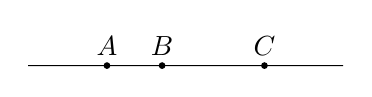
\begin{tikzpicture}
\draw[fill=black] (0,0)--(1,0)node[above]{\(A\)}circle(1pt)
--(1.7,0)node[above]{\(B\)}circle(1pt)
--(3,0)node[above]{\(C\)}circle(1pt)
--(4,0);
\end{tikzpicture}
\caption{直线上点的顺序}
\label{figure:欧式几何.直线上点的顺序1}
\end{figure}

\item 对于两点\(A\)和\(B\)(如\cref{figure:欧式几何.直线上点的顺序2} ),直线\(AB\)上恒至少有一点\(C\),使得\(B\)在\(A\)和\(C\)之间.
\begin{figure}[ht]
\centering
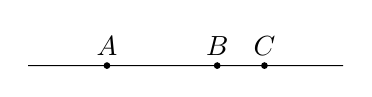
\begin{tikzpicture}
\draw[fill=black] (0,0)--(1,0)node[above]{\(A\)}circle(1pt)
--(2.4,0)node[above]{\(B\)}circle(1pt)
--(3,0)node[above]{\(C\)}circle(1pt)
--(4,0);
\end{tikzpicture}
\caption{直线上点的顺序}
\label{figure:欧式几何.直线上点的顺序2}
\end{figure}

\item 一直线的任意三点中,至多有一点在其他两点之间.
\end{enumerate}
\end{axiom}

在上述三条\textbf{直线顺序公理}之外,还需要一条\textbf{平面顺序公理}.

\begin{axiom}[顺序公理II]\label{axiom:欧式几何.顺序公理2}
考虑一直线\(l\)上的两点\(A\)和\(B\).
我们把这一对点\(A\)和\(B\)确定的介于它们的点的集合叫做一条\textbf{线段},记作\(AB\)(或\(BA\)).
在\(A\)和\(B\)之间的点叫做线段\(AB\)的点,或线段\(AB\)的\textbf{内点};
\(A\)和\(B\)叫做线段\(AB\)的\textbf{端点};
直线\(l\)上的其他点叫做线段\(AB\)的\textbf{外点}.
\begin{enumerate}
\setcounter{enumi}{3}
\item 设\(A\)、\(B\)和\(C\)是不在同一直线上的三点,\(l\)是平面\(ABC\)上的一直线,但\(l\)不通过\(A,B,C\)这三点中的任一点(如\cref{figure:欧式几何.平面上点的顺序1} ),若直线\(l\)通过线段\(AB\)的一点,则它必定也通过线段\(AC\)或线段\(BC\)的一点.
\begin{figure}[ht]
\centering
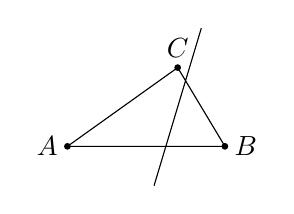
\begin{tikzpicture}
\draw[fill=black] (-1,0)node[left]{\(A\)}circle(1pt)
--(1,0)node[right]{\(B\)}circle(1pt)
--(.4,1)node[above]{\(C\)}circle(1pt)--(-1,0)
(.1,-.5)--(.7,1.5);
\end{tikzpicture}
\caption{平面上点的顺序}
\label{figure:欧式几何.平面上点的顺序1}
\end{figure}
\end{enumerate}
\end{axiom}
直观地说,\cref{axiom:欧式几何.顺序公理2} 说的就是:若一直线“冲进”一个三角形的内部,它必定还要再“冲出”这个三角形.
易证:与线段\(AB\)相交的直线\(l\)不同时和\(AC,BC\)这两条线段都相交.

\subsection{关联公理和顺序公理的推论}
从\cref{axiom:欧式几何.关联公理,axiom:欧式几何.顺序公理1,axiom:欧式几何.顺序公理2} 能推证下列定理.
\begin{theorem}\label{theorem:欧式几何.定理3}
对于两点\(A\)和\(C\),直线\(AC\)上恒至少有一点\(D\),在\(A\)和\(C\)之间.
\begin{proof}
根据\cref{axiom:欧式几何.关联公理} 第3条,直线\(AC\)外存在一点\(E\);
根据\cref{axiom:欧式几何.顺序公理1} 第2条,直线\(AE\)上有一点\(F\),使得\(E\)在线段\(AF\)内.
根据\cref{axiom:欧式几何.顺序公理1} 第2条、第3条,直线\(FC\)上有一点\(G\),不在线段\(FC\)内.
根据\cref{axiom:欧式几何.顺序公理2} 第4条,直线\(EG\)必交线段\(AC\)于一点\(D\).
\end{proof}
\end{theorem}

\begin{theorem}\label{theorem:欧式几何.定理4}
一直线上的任意三点\(A,B,C\)中,必有一点且只有一点在其他两点之间.
\begin{proof}
设\(A\)不在\(B\)和\(C\)之间,而且\(C\)不在\(A\)和\(B\)之间.
用直线连接\(B\)和直线\(AC\)外一点\(D\).
根据\cref{axiom:欧式几何.顺序公理1} 第2条,能在直线\(BD\)上取一点\(G\),使得\(D\)在\(B\)和\(G\)之间.
对于三角形\(BCG\)和直线\(AD\)应用\cref{axiom:欧式几何.顺序公理2} 第4条,可知直线\(AD\)通过线段\(CG\)内的一点\(E\);
同理可知直线\(CD\)通过线段\(AG\)内一点\(F\).
对于三角形\(AEG\)和直线\(CF\)应用\cref{axiom:欧式几何.顺序公理2} 第4条,可知\(D\)在\(A\)和\(E\)之间;
再对于三角形\(AEC\)和直线\(BG\)应用\cref{axiom:欧式几何.顺序公理2} 第4条,即证得\(B\)在\(A\)和\(C\)之间.
\end{proof}
\end{theorem}

\begin{theorem}\label{theorem:欧式几何.定理5}
一直线上的任意四点\(A,B,C,D\),使得点\(B\)既在\(A\)和\(C\)之间,又在\(A\)和\(D\)之间;
而且点\(C\)既在\(A\)和\(D\)之间,又在\(B\)和\(D\)之间.
\end{theorem}

\begin{corollary}\label{theorem:欧式几何.定理6}
一直线上的任意有限个点\(A,B,C,\dotsc,K\),%
使得点\(B\)在\(A\)和\(C\),或和\(D\),或和\(E\),……,或和\(K\)之间;
而且点\(C\)在\(A\)(或\(B\))和\(D\),或和\(E\),……,或和\(K\)之间;以此类推.
\end{corollary}

\begin{corollary}\label{theorem:欧式几何.定理7}
一直线上任意两点之间恒有无限多个点.
\end{corollary}

\begin{theorem}\label{theorem:欧式几何.定理8}
一平面\(\gamma\)上的任一直线\(l\)将该平面上其余的点分为具有下述性质的两个区域:
一个区域的任一点\(A\)与另一区域的任一点\(B\)所决定的线段\(AB\)内,%
必含有直线\(l\)的一点(如\cref{figure:欧式几何.直线l分平面为两个区域} );%
而同一个区域的任意两点\(A\)和\(A'\)所决定的线段\(AA'\)内,不含有直线\(l\)的点.
\begin{figure}[ht]
\centering
\begin{tikzpicture}
\draw (-2,0)--(2,0)node[right]{\(l\)}
(.5,-1)node[right]{\(B\)}--(-.5,.5)node[left]{\(A\)}--(.3,1)node[right]{\(A'\)};
\end{tikzpicture}
\caption{直线\(l\)分平面为两个区域}
\label{figure:欧式几何.直线l分平面为两个区域}
\end{figure}
\end{theorem}

\begin{definition}
我们说\(A\)和\(A'\)这两点在平面\(\gamma\)上直线\(l\)的\textbf{同侧}%
(如\cref{figure:欧式几何.直线l分平面为两个区域} ),%
而\(A\)和\(B\)这两点在平面\(\gamma\)上直线\(l\)的\textbf{异侧}.%
\end{definition}

\begin{definition}
设\(A,A',O\)和\(B\)是一直线\(l\)上的四点(如\cref{figure:欧式几何.射线} ),%
而\(O\)在\(A\)和\(B\)之间,但不在\(A\)和\(A'\)之间.
我们称“\(A\)和\(A'\)这两点在\(l\)上点\(O\)的\textbf{同侧}”,%
而称“\(A\)和\(B\)这两点在\(l\)上点\(O\)的\textbf{异侧}”.

直线\(l\)上点\(O\)的同侧的点的全体,叫做从点\(O\)起始的一条\textbf{射线};
因此一直线的每一点把这直线分成两条射线.
\begin{figure}[ht]
\centering
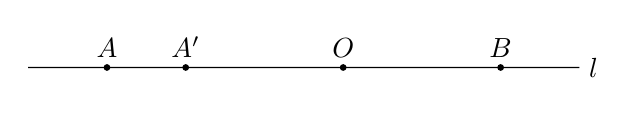
\begin{tikzpicture}
\draw[fill=black] (-3,0)--(-2,0)node[above]{\(A\)}circle(1pt)
--(-1,0)node[above]{\(A'\)}circle(1pt)
--(1,0)node[above]{\(O\)}circle(1pt)
--(3,0)node[above]{\(B\)}circle(1pt)--(4,0)node[right]{\(l\)};
\end{tikzpicture}
\caption{射线}
\label{figure:欧式几何.射线}
\end{figure}
\end{definition}

\begin{definition}
若干条首尾相连的线段\(AB,BC,CD,\dotsc,KL\)的集合叫做一条\textbf{折线段},它连结\(A\)和\(L\)这两点.
为求简便,可将这条折线段记为\(ABCD \dotso KL\).
线段\(AB,BC,CD,\dotsc,KL\)的内点和端点都叫做这条折线段的点.

若点\(A,B,C,D,\dotsc,K,L\)都在同一平面上,且\(L\)和\(A\)是同一个点,则该折线段就叫做一个\textbf{多边形},记为\(ABCD \dotso K\);线段\(AB,BC,CD,\dotsc,KA\)叫做这多边形的\textbf{边};点\(A,,B,C,D,\dotsc,K\)叫做多边形的\textbf{顶点}.

若一个多边形有三个顶点,则称之为\textbf{三角形}.
若一个多边形有\(n\ (n>3)\)个顶点,则称之为\(n\)\textbf{边形}.
若一个多边形的顶点各各不同,它的任一边内不含有顶点,且它的任意两边无公共点,这个多边形就叫做\textbf{简单多边形}.
\end{definition}

根据\cref{theorem:欧式几何.定理8} 可以推出下列两条推论:
\begin{corollary}\label{theorem:欧式几何.定理9}
一平面\(\alpha\)上的每一个简单多边形,把平面\(\alpha\)上其余点分为\textbf{内域}和\textbf{外域}两个区域.
这两个区域具有如下性质:
若\(A\)是内域的一个点(内点),而且\(B\)是外域的一个点(外点),则平面\(\alpha\)上任意一条连接\(A\)和\(B\)的折线段,至少和多边形有一公共点;
若\(A\)和\(A'\)是内点,而\(B\)和\(B'\)是外点,则在平面\(\alpha\)上恒有连接\(A\)和\(A'\)的折线段,和连接\(B\)和\(B'\)的折线段,它们都和多边形无公共点;
平面\(\alpha\)上存在全含于外域的直线,而不存在全含于内域的直线.
\end{corollary}

\begin{corollary}\label{theorem:欧式几何.定理10}
每一平面\(\alpha\)把空间中其余点分为具有下述性质的两个区域:
一区域的任一点\(A\)和另一区域的任一点\(B\)所决定的线段\(AB\)内,必含有\(\alpha\)的一点;
同一区域的任意两点\(A\)和\(A'\)所决定的线段\(AA'\)内,恒不含有\(\alpha\)的点.
\end{corollary}

\begin{definition}
在\cref{theorem:欧式几何.定理10} 的条件下,我们说\(A\)和\(A'\)这两点在空间中平面\(\alpha\)的\textbf{同侧},而\(A\)和\(B\)这两点在空间中平面\(\alpha\)的\textbf{异侧}.
\end{definition}

\subsection{第三组公理:合同公理}
本组公理规定“合同”这个概念,利用它就可以规定运动的概念.

\begin{axiom}[合同公理]\label{axiom:欧式几何.合同公理}
线段间有一定的相互关系,我们用“合同”或“相等”这个词来描述.
\begin{enumerate}
\item 设\(A\)和\(B\)是一直线\(a\)上的两点,\(A'\)是这直线或另一直线\(a'\)上的一点,而且给定了直线\(a'\)上\(A'\)的一侧,则在直线\(a'\)上\(A'\)的这一侧,恒有一点\(B'\),使得线段\(AB\)和线段\(A'B'\)合同或相等;我们将上述关系记为\(AB \equiv A'B'\).

\item 若两线段\(A'B'\)和\(A''B''\)都和线段\(AB\)合同,则\(A'B'\)和\(A''B''\)也合同.

\item 设两线段\(AB\)和\(BC\)在同一直线\(a\)上,无公共点,而且两线段\(A'B'\)和\(B'C'\)在这直线或另一直线\(a'\)上亦无公共点.若\(AB \equiv A'B'\)且\(BC \equiv B'C'\),则\(AC \equiv A'C'\).
\end{enumerate}
\end{axiom}
\cref{axiom:欧式几何.合同公理} 第3条要求线段能够相加.

\begin{property}
线段的合同关系具有对称性和传递性,即\begin{enumerate}
\item \textbf{对称性},\(AB \equiv A'B' \implies A'B' \equiv AB\)\footnote{%
正因线段的合同关系具有对称性,我们才能说“某两条线段\textbf{互相合同}”.%
}
.
\item \textbf{传递性},\(AB \equiv A'B' \land A'B' \equiv A''B'' \implies AB \equiv A''B''\).
\end{enumerate}
\end{property}

\subsection{第四组公理:平行公理}

\begin{axiom}[平行公理]
两直线被第三条直线所截,如果同侧两内角和小于两个直角, 则两直线则会在该侧相交.
\end{axiom}

\subsection{第五组公理:连续公理}

\begin{axiom}[连续公理]
\end{axiom}

\section{平面三角形}

\begin{theorem}
三角形内角和为\(\pi\).
\begin{proof}
如下图,有\(\triangle ABC\).过点\(C\)作平行于线段\(AB\)的直线\(PQ\).
\begin{center}
\begin{tikzpicture}
\coordinate (A) at (0,0);
\coordinate (B) at (4,0);
\coordinate (C) at (3,2);
\coordinate (P) at (2,2);
\coordinate (Q) at (4,2);
\draw (A)node[left]{\(A\)} -- (B)node[right]{\(B\)} -- (C)node[above]{\(C\)} -- (A);
\draw (P)node[left]{\(P\)} -- (Q)node[right]{\(Q\)};
\draw pic[draw=blue,angle radius=5mm]{angle=B--A--C}
		pic[draw=blue,angle radius=6mm]{angle=B--A--C}
		pic[draw=blue,angle radius=5mm]{angle=P--C--A}
		pic[draw=blue,angle radius=6mm]{angle=P--C--A}
		pic[draw=orange,angle radius=4mm]{angle=C--B--A}
		pic[draw=orange,angle radius=4mm]{angle=B--C--Q};
\end{tikzpicture}
\end{center}
由内错角相等,有\[
\angle{PCA} = \angle{CAB}, \quad \angle{QCB} = \angle{CBA},
\]又由\(\angle{PCA}+\angle{ACB}+\angle{QCB}=\pi\),可得\[
\angle{CAB}+\angle{ACB}+\angle{QCB}=\pi.
\qedhere
\]
\end{proof}
\end{theorem}

\begin{theorem}[正弦定理]
设任意三角形\(\triangle ABC\)的外接圆半径为\(R\),则\begin{equation}
\frac{a}{\sin A}
= \frac{b}{\sin B}
= \frac{c}{\sin C}
= 2R.
\end{equation}
\end{theorem}

\begin{theorem}[余弦定理]
设任意三角形\(\triangle ABC\),有\begin{equation}
c^2 = a^2 + b^2 - 2ab \cos C.
\end{equation}
\end{theorem}
可以看出,勾股定理是余弦定理的特殊情况,即当\(C = \frac{\pi}{2}\)时,有\(\cos C=0\),于是\(c^2 = a^2 + b^2\).

\begin{theorem}[摩尔外德公式]
%@see: https://mathshistory.st-andrews.ac.uk/Biographies/Mollweide/
%@see: https://arxiv.org/pdf/1808.08049.pdf
设任意三角形\(\triangle ABC\),则\begin{gather}
\frac{a+b}{c}
= \frac{\cos[(A-B)/2]}{\sin(C/2)}, \\
\frac{a-b}{c}
= \frac{\sin[(A-B)/2]}{\cos(C/2)}.
\end{gather}
\end{theorem}

\begin{theorem}[正切定理]
设任意三角形\(\triangle ABC\),有\begin{equation}
\frac{a-b}{a+b} = \frac{\tan[(A-B)/2]}{\tan[(A+B)/2]}.
\end{equation}
\end{theorem}

\section{圆}
\subsection{圆的概念}
\subsection{圆的性质}
\subsection{圆的周长\ 圆周率}
\begin{definition}
定义:圆的周长\(C\)与其直径\(2R\)之比称为\textbf{圆周率},记作\(\pi\),即\[
\pi = \frac{C}{2R}.
\]
\end{definition}
由于圆周率是一个常数,那么已知圆的直径(或半径)可以求得圆的周长,而已知圆的周长可以求得圆的直径(或半径).

\begin{property}
给定圆上任意一段弧,若它的角度为\(\theta\),那么弧长为\(\theta r\).
\end{property}

\begin{corollary}
如下图,在单位圆上,当圆弧的角度\(\theta\)为锐角,即\(0<\theta<\pi/2\)时,\(\theta > x\). \begin{center}
\begin{tikzpicture}[scale=4]
%\draw[help lines, color=gray!30, dashed] (0,0) grid (1,1);
\pgfmathsetmacro{\u}{sqrt(3)/2}
\coordinate (O) at (0,0);
\coordinate (A) at (\u,0);
\coordinate (B) at (\u,1/2);
\draw (1,0)arc[start angle=0,end angle=30,radius=1]node[midway,right]{\(\theta\)} -- (0,0)node[midway,above left]{\(1\)} -- (1,0)
	(A) -- (B)node[midway,left]{\(x\)};
\draw pic["\(\theta\)",draw=orange,-,angle eccentricity=1.7,angle radius=5mm]{angle=A--O--B} pic[draw=gray,-,angle radius=0.3cm]{right angle=B--A--O};
\end{tikzpicture}
\end{center}
\end{corollary}

\section{平面凸多边形}
\begin{theorem}
设凸多边形的边数为\(n\),则其内角和为\((n-2)\pi\).
\end{theorem}
如图,在凸多边形内部任取一点\(P\),连接该点与凸多边形各顶点,可以得到\(n\)个三角形.
因为三角形内角和为\(\pi\),所以\(n\)个三角形内角和的总和为\(n\pi\),再减去各三角形\(\angle P\)之和\(2\pi\),可知凸\(n\)边形的内角和为\((n-2)\pi\).
\begin{center}
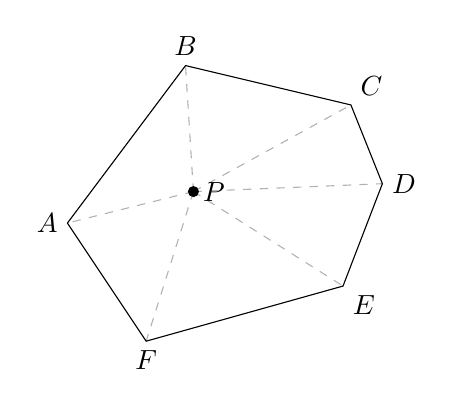
\begin{tikzpicture}
\coordinate (A1) at (0,2);
\coordinate (A2) at (1.5,4);
\coordinate (A3) at (3.6,3.5);
\coordinate (A4) at (4,2.5);
\coordinate (A5) at (3.5,1.2);
\coordinate (A6) at (1,0.5);
\coordinate (P) at (1.6,2.4);
\draw[dashed,color=black!30] (P)--(A1) (P)--(A2) (P)--(A3) (P)--(A4) (P)--(A5) (P)--(A6);
\draw (A1)node[left]{\(A\)}--(A2)node[above]{\(B\)}--(A3)node[above right]{\(C\)}--(A4)node[right]{\(D\)}--(A5)node[below right]{\(E\)}--(A6)node[below]{\(F\)}--(A1) (P)node[right]{\(P\)};
\fill (P)circle(2pt);
\end{tikzpicture}
\end{center}

\begin{theorem}
凸多边形的外角和为\(2\pi\).
\end{theorem}

\section{凸多面体}
\begin{theorem}[欧拉公式]
设凸多面体的顶点数、棱数、面数分别为\(V\)、\(E\)、\(F\),则有\[
V - E + F = 2.
\]
\end{theorem}

\begin{definition}
\textbf{正凸多面体}(简称\textbf{正多面体}),是指满足以下条件的凸多面体:
\begin{enumerate}
\item 正多面体的面由正多边形构成;
\item 正多面体的各个顶角相等;
\item 正多面体的各条棱长相等.
\end{enumerate}
\end{definition}

\begin{corollary}
正凸多面体只有5种:三四面体、正方体、正八面体、正十二面体、正二十面体.
\end{corollary}


\chapter{解析几何}
古希腊的毕达哥拉斯曾经提出“万物皆数”这一哲学观点,从这一章开始,我们研究如何利用代数方法研究几何问题.

在利用函数图像研究初等函数的性质时,我们产生了这么一个观念:
在平面上建立了平面直角坐标系以后,
平面上的点与数是一一对应的,
或说平面上的点与由实有序对\((x,y)\)一一对应.
几何图形是由点构成的集合,我们自然地想到能不能用数的集合来代表几何图形.
这就是解析几何的思想根源.

\section{平面二次曲线及其方程}

\subsection{平面曲线在极坐标系下方程}
在平面内取一个定点\(O\),称为\DefineConcept{极点}.
过极点引一条射线\(Ox\),称为\DefineConcept{极轴}.
再选一个长度单位和计算角度的正方向(通常取逆时针方向),
这样的坐标系称为\DefineConcept{极坐标系}.
连接平面内任意一点\(P\)与极点\(O\)所得的线段\(OP\),称为“点\(P\)的\DefineConcept{极径}”.
这条线段\(OP\)与极轴所得的夹角\(\angle POx\),称为“点\(P\)的\DefineConcept{极角}”.

\begin{table}[htb]
	\centering
	\begin{tblr}{c|c|c}
		\hline
		& 直角坐标方程
		& 极坐标方程 \\ \hline
		过极点的直线的方程
			& \(y = x \tan\theta_0\)
			& \(\theta=\theta_0\ (\text{$\theta_0$是常数})\) \\
		垂直于极轴的直线的方程
			& \(x = a\)
			& \(\rho\cos\theta=a\) \\
		平行于极轴的直线的方程
			& \(y = a\)
			& \(\rho\sin\theta=a\) \\
			& \(x + y = a\)
			& \(\rho = \frac{a}{\cos\theta + \sin\theta}\) \\
		中心在极点、半径为\(r\)的圆
			& \(x^2+y^2=r^2\)
			& \(\rho=r\) \\
		中心在\((r,0)\)、半径为\(r\)的圆
			& \((x-r)^2+y^2=r^2\)
			& \(\rho=2r\cos\theta\) \\
		中心在\((r,\pi)\)、半径为\(r\)的圆
			& \((x+r)^2+y^2=r^2\)
			& \(\rho=-2r\cos\theta\) \\
		中心在\((\rho_0,\theta_0)\)、半径为\(r\)的圆
			&
			& \(\rho^2+\rho_0^2-2\rho_0\rho\cos(\theta-\theta_0)=r^2\) \\
		\hline
	\end{tblr}
	\caption{}
\end{table}


\section{本章总结}

\subsection*{常见的坐标系}
极坐标系是一种平面坐标系.
极坐标系上的点\((\rho,\theta)\)与平面直角坐标系上的点\((x,y)\)存在以下的一一对应关系:\begin{equation*}
\left\{ \begin{array}{l}
x = \rho\cos\theta, \\
y = \rho\sin\theta. \\
\end{array} \right.
\end{equation*}

柱面坐标系是一种空间坐标系.
柱面坐标系上的点\((\rho,\theta,z)\)与空间直角坐标系上的点\((x,y,z)\)存在以下的一一对应关系:\begin{equation*}
\left\{ \begin{array}{l}
x = \rho\cos\theta, \\
y = \rho\sin\theta, \\
z = z. \\
\end{array} \right.
\end{equation*}

球极坐标系是一种空间坐标系.
球极坐标系上的点\((r,\theta,\phi)\)与空间直角坐标系上的点\((x,y,z)\)存在以下的一一对应关系:\begin{equation*}
\left\{ \begin{array}{l}
x = r \sin\phi \cos\theta, \\
y = r \sin\phi \sin\theta, \\
z = r \cos\phi. \\
\end{array} \right.
\end{equation*}

\begin{figure}[h]
	\centering
	\begin{tikzpicture}
		\coordinate (O) at (0,0);
		\coordinate (M) at (2,2);
		\coordinate (P) at (2,-1.2);
		\coordinate (A) at (-0.8,-1.2);
		\coordinate (Z) at (0,1);
		\draw (O)node[left]{\(O\)}
				-- (M)node[right]{\(M\)} node[midway,above]{\(r\)}
				-- (P)node[right]{\(P\)} node[midway,right]{\(z\)}
				-- (A)node[left]{\(A\)} node[midway,below]{\(y\)}
				-- (O)node[midway,left]{\(x\)}
			(O) -- (P)
			pic["\(\phi\)",draw=orange,<-,angle eccentricity=1.3,angle radius=0.6cm]{angle=M--O--Z}
			pic["\(\theta\)",draw=orange,->,angle eccentricity=1.5,angle radius=0.4cm]{angle=A--O--P};
		\begin{scope}[>=Stealth,->,ultra thick]
			\draw(0,0) -- (-1.5,-2.25) node[right]{\(x\)};
			\draw(0,0) -- (3,0) node[right]{\(y\)};
			\draw(0,0) -- (0,3) node[above]{\(z\)};
		\end{scope}
	\end{tikzpicture}
	\caption{球极坐标系}
\end{figure}


\chapter{函数}
\section{函数的概念}
\subsection{一元函数的概念}
设\(D\)是\(\mathbb{R}\)的一个非空子集,
称映射\(f\colon D \to \mathbb{R}\)为
“定义在\(D\)上的一个\DefineConcept{一元函数}”,
简称\DefineConcept{函数},通常记为\[
	y = f(x), \qquad x \in D,
\]
其中点集\(D\)称为该函数的\DefineConcept{定义域},
\(x\)称为\DefineConcept{自变量},
\(y\)称为\DefineConcept{因变量}.

函数定义中,对每个\(x \in D\),
按对应法则\(f\),总有唯一确定的值\(y\)与之相应,
这个值称为函数\(f\)在\(x\)处的\DefineConcept{函数值},
记作\(f(x)\),即\(y=f(x)\).
因变量\(y\)与自变量\(x\)之间的这种依赖关系,通常称为\DefineConcept{函数关系}.
函数值\(f(x)\)的全体所构成的集合称为函数\(f\)的\DefineConcept{值域},
记作\(R_f\)或\(f\ImageOfSetUnderRelation{D}\),即\[
	R_f = f\ImageOfSetUnderRelation{D} = \Set{ y \given y = f(x) \land x \in D }.
\]

函数的定义域通常按以下两种情形来确定:
\begin{itemize}
	\item 一种是对有实际背景的函数,
	根据实际背景中变量的实际意义来确定.
	\item 另一种是对抽象地用算式表达的函数,
	通常约定这种函数的定义域是使得算式有意义的一切实数组成的集合,
	这种定义域称为函数的\DefineConcept{自然定义域}.
\end{itemize}

\begin{example}
函数\(y = \frac{1}{x}\)的自然定义域是
\(\Set{ x \in \mathbb{R} \given x \neq 0 }\).
\end{example}

\begin{example}
函数\(y = \sqrt{x}\)的自然定义域是
\(\Set{ x \in \mathbb{R} \given x \geq 0 }\).
\end{example}

如果给定一个对应法则,按这个法则,
对每个\(x \in D\),总有确定但不唯一的\(y\)与之对应.
这样的不符合函数的定义的对应法则,
习惯上称这种法则确定了一个\DefineConcept{多值函数}.
对于多值函数,如果我们附加一些条件,使得在附加条件之下,按照这个法则,
对每个\(x \in D\),总有唯一确定的实数值\(y\)与之对应,那么这就确定了一个函数.
我们称这样得到的函数为多值函数的\DefineConcept{单值分支}.

\subsection{多元函数的概念}
\begin{definition}
设\(D\)是\(\mathbb{R}^2\)的一个非空子集,
称映射\(f\colon D \to \mathbb{R}\)为
“定义在\(D\)上的\DefineConcept{二元函数}”,
通常记为\[
	z = f(x,y),
	\quad \opair{x,y} \in D
\]或\[
	z = f(P),
	\quad P\opair{x,y} \in D
\]
其中点集\(D\)称为该函数的\DefineConcept{定义域},
\(x\)、\(y\)称为\DefineConcept{自变量},
\(z\)称为\DefineConcept{因变量}.
\end{definition}

\begin{definition}
类似地,设\(D\)是\(n\)维空间\(\mathbb{R}^n\)的一个非空子集,
称映射\[
	f\colon D \to \mathbb{R}
\]
为“定义在\(D\)上的\(n\)元\DefineConcept{函数}”,
通常记为\[
	y = f(\AutoTuple{x}{n}),
	\quad \opair{\AutoTuple{x}{n}} \in D
\]或\[
	y = f(\mat{x}),
	\quad \mat{x}=\opair{\AutoTuple{x}{n}} \in D
\]
其中点集\(D\)称为“函数\(f\)的\DefineConcept{定义域}”,
\(x\)、\(y\)称为“函数\(f\)的\DefineConcept{自变量}”,
\(z\)称为“函数\(f\)的\DefineConcept{因变量}”.
\end{definition}

\section{函数的性质}
\subsection{函数的有界性}
\begin{definition}\label{definition:函数.函数的有界性}
%@see: 《数学分析(上册)》(陈纪修) P19 定义1.2.3
设函数\(f\)的定义域为\(D\),数集\(X \subseteq D\).

如果存在数\(K_1\),使得\(f(x) \leq K_1\)对任一\(x \in X\)都成立,即\[
	(\forall x \in X)
	(\exists K_1 \in \mathbb{R})
	[f(x) \leq K_1],
\]
则称“函数\(f\)在\(X\)上有\DefineConcept{上界}”,
称“\(K_1\)是函数\(f\)在\(X\)上的一个上界”.

如果存在数\(K_2\),使得\(f(x) \geq K_2\)对任一\(x \in X\)都成立,即\[
	(\forall x \in X)
	(\exists K_2 \in \mathbb{R})
	[f(x) \geq K_2],
\]
则称“函数\(f\)在\(X\)上有\DefineConcept{下界}”,
称“\(K_2\)是函数\(f\)在\(X\)上的一个下界”.

如果存在正数\(M\),使得\(\abs{f(x)} \leq M\)对任一\(x \in X\)都成立,即\[
	(\forall x \in X)
	(\exists M>0)[
		\abs{f(x)} \leq M
	],
\]
则称“函数\(f\)在\(X\)上\DefineConcept{有界}”
或“函数\(f\)是\(X\)上的\DefineConcept{有界函数}”.
反之如果这样的\(M\)不存在,即\[
	(\exists x_0 \in X)
	(\forall M>0)[
		\abs{f(x_0)} > M
	],
\]
就称“函数\(f\)在\(X\)上\DefineConcept{无界}”.
\end{definition}

应该注意到,当一个函数有界时,它的上界、下界均不唯一.
对于一个上界为\(M\)、下界为\(m\)的函数,
任意小于\(m\)的数都是它的下界,
任意大于\(M\)的数都是它的上界.

\begin{theorem}
设函数\(f\)的定义域为\(D\),数集\(X \subseteq D\).
函数\(f\)在\(X\)上有界的充分必要条件是它在\(X\)上既有上界又有下界.
\end{theorem}

\subsection{函数的单调性}
\begin{definition}
%@see: 《数学分析(上册)》(陈纪修) P20 定义1.2.4
设函数\(f\)的定义域为\(D\),区间\(I \subseteq D\).
\begin{itemize}
	\item 如果\[
		(\forall x_1,x_2\in I)
		[x_1 < x_2 \implies f(x_1) \leq f(x_2)],
	\]
	则称“函数\(f\)在区间\(I\)上是\DefineConcept{单调增加的}”.

	\item 如果\[
		(\forall x_1,x_2\in I)
		[x_1 < x_2 \implies f(x_1) < f(x_2)],
	\]
	则称“函数\(f\)在区间\(I\)上是\DefineConcept{严格单调增加的}”.

	\item 如果\[
		(\forall x_1,x_2\in I)
		[x_1 < x_2 \implies f(x_1) \geq f(x_2)],
	\]
	则称“函数\(f\)在区间\(I\)上是\DefineConcept{单调减少的}”.

	\item 如果\[
		(\forall x_1,x_2\in I)
		[x_1 < x_2 \implies f(x_1) > f(x_2)],
	\]
	则称“函数\(f\)在区间\(I\)上是\DefineConcept{严格单调减少的}”.
\end{itemize}

单调增加的函数和单调减少的函数统称为\DefineConcept{单调函数}(monotonic function).
%@see: https://mathworld.wolfram.com/MonotonicFunction.html
\end{definition}

\begin{proposition}
“\(f\)是单调函数”是“\(f\)是单射”的充分不必要条件.
\end{proposition}

\subsection{函数的奇偶性}
\begin{definition}
%@see: 《数学分析(上册)》(陈纪修) P20 定义1.2.5
设函数\(f\)定义域\(D\)关于原点对称,即\((\forall x)[x \in D \iff -x \in D]\).
\begin{itemize}
	\item 若\((\forall x \in D)
	[f(-x) = f(x)]\),
	则称“\(f(x)\)是\DefineConcept{偶函数}”.

	\item 若\((\forall x \in D)
	[f(-x) = -f(x)]\),
	则称“\(f(x)\)是\DefineConcept{奇函数}”.
\end{itemize}
\end{definition}

\begin{property}
偶函数的图形是关于\(y\)轴对称的.
奇函数的图形是关于原点对称的.
\end{property}

\begin{property}
奇函数与奇函数之和、之差均为奇函数.
偶函数与偶函数之和、之差均为偶函数.
\begin{proof}
设\[
f(-x) = -f(x), \qquad g(-x) = -g(x).
\]令\(F(x) = f(x) \pm g(x)\),则\[
F(-x) = f(-x) \pm g(-x)
= [-f(x)] \pm [-g(x)]
= -[f(x) \pm g(x)]
= -F(x).
\qedhere
\]
\end{proof}
\end{property}

\begin{property}
奇函数与奇函数之积为偶函数.
\begin{proof}
设\[
f(-x) = -f(x), \qquad g(-x) = -g(x).
\]令\(F(x) = f(x) \cdot g(x)\),则\[
F(-x) = f(-x) \cdot g(-x)
= [-f(x)] \cdot [-g(x)]
= f(x) \cdot g(x)
= F(x).
\qedhere
\]
\end{proof}
\end{property}

\begin{property}
奇函数与偶函数之积为奇函数.
\begin{proof}
设\[
f(-x) = -f(x), \qquad g(-x) = g(x).
\]令\(F(x) = f(x) \cdot g(x)\),则\[
F(-x) = f(-x) \cdot g(-x)
= [-f(x)] \cdot g(x)
= - f(x) \cdot g(x)
= - F(x).
\qedhere
\]
\end{proof}
\end{property}

\begin{property}
偶函数与偶函数之积为偶函数.
\begin{proof}
设\[
f(-x) = f(x), \qquad g(-x) = g(x).
\]令\(F(x) = f(x) \cdot g(x)\),则\[
F(-x) = f(-x) \cdot g(-x) = f(x) \cdot g(x) = F(x).
\qedhere
\]
\end{proof}
\end{property}

\begin{example}\label{example:函数.任一函数可拆为奇偶函数之和}
试证:任意一个函数总可分解为一个奇函数与一个偶函数之和.
\begin{proof}
设函数\(f\colon(-l,l)\to\mathbb{R}\),其中\(l>0\).
假设在\((-l,l)\)上存在偶函数\(g\)和奇函数\(h\),
使得\[
	(\forall x)
	[-l<x<l \implies f(x) = g(x)+h(x)].
\]
那么可以建立关于\(g(x),h(x)\)的方程\[
	\left\{ \begin{array}{l}
		f(x) = g(x) + h(x), \\
		f(-x) = g(-x) + h(-x) = g(x) - h(x).
	\end{array} \right.
\]
解得\[
	g(x) = \frac12 [f(x) + f(-x)], \qquad
	h(x) = \frac12 [f(x) - f(-x)].
\]
可以验证:\[
	g(-x) = \frac12 [f(-x) + f(x)] = g(x), \qquad
	h(-x) = \frac12 [f(-x) - f(x)] = -h(x).
\]
也就是说,\(g\)是偶函数,\(h\)是奇函数.
\end{proof}
\end{example}

\subsection{函数的周期性}
\begin{definition}
%@see: 《数学分析(上册)》(陈纪修) P20 定义1.2.6
设函数\(f\colon D\to\mathbb{R}\).
如果存在一个常数\(T>0\),
使得\[
	(\forall x \in D)
	[x+T \in D \implies f(x+T) = f(x)],
\]
则称“\(f\)是(以\(T\)为周期的)\DefineConcept{周期函数}”
“\(T\)是\(f\)的周期”.

如果以\(T\)为周期的周期函数\(f\)满足\[
	(\forall a\in\mathbb{R})
	[0<a<T \implies f(x+a) \neq f(x)],
\]
则称“\(T\)为\DefineConcept{最小正周期}”.
\end{definition}

\begin{example}
狄利克雷函数\[
	D(x) = \left\{ \begin{array}{ll}
		1, & x \in \mathbb{Q}, \\
		0, & x \in \mathbb{R}-\mathbb{Q}.
	\end{array} \right.
\]是一个周期函数,任何正有理数\(r\)都是它的周期.
因为不存在最小的正有理数,所以它没有最小正周期.
\end{example}

\begin{example}
设函数\(f\colon\mathbb{R}\to\mathbb{R}\)满足\[
	f(x+a) = -f(x),
	\quad a\neq0,
\]
证明:函数\(f\)的周期为\(2a\).
\begin{proof}
易见\(f(x+2a)
=f((x+a)+a)
=-f(x+a)
=f(x)\).
\end{proof}
\end{example}

\begin{example}
设函数\(f\colon\mathbb{R}\to\mathbb{R}\)同时满足\[
	f(x)=f(2a-x)
	\quad\text{和}\quad
	f(x)=f(2b-x),
\]
证明:函数\(f\)的周期为\(2\abs{a-b}\).
\begin{proof}
易见\(f(x)
=f(2a-x)
=f(2b-x)\).
令\(t=2b-x\),
得\(x=2b-t\),
故\(f(2a-(2b-t))=f(t)\),
即\(f(t)=f(t+2(a-b))\).
\end{proof}
\end{example}

\begin{example}
设函数\(f\colon\mathbb{R}\to\mathbb{R}\)同时满足\[
	f(x)+f(2a-x)=0
	\quad\text{和}\quad
	f(x)=f(2b-x),
\]
证明:函数\(f\)的周期为\(4\abs{a-b}\).
\begin{proof}
易见\(f(2b-x)+f(2a-x)=0\).
令\(t=2b-x\),
则\[
	f(t)+f(2a-(2b-t))
	=f(t)+f(t+2(a-b))
	=0.
	\qedhere
\]
\end{proof}
\end{example}

\begin{example}
设函数\(f\colon\mathbb{R}\to\mathbb{R}\)满足\[
	f(x+a)=\pm\frac1{f(x)},
\]
证明:函数\(f\)的周期为\(2\abs{a}\).
\begin{proof}
易见\(f(x+2a)=\pm\frac1{f(x+a)}=f(x)\).
\end{proof}
\end{example}

\section{反函数与复合函数}
\subsection{反函数}
根据\cref{theorem:集合论.关系及其逆是映射的充分必要条件},
当函数\(f\colon X \to Y\)是单射时,
它有逆映射\(f^{-1}\).
\(f^{-1}\)的定义域和值域分别为\(Z=\ran f\)和\(\dom f=X\).
我们把这个逆映射称为“函数\(f\)的\DefineConcept{反函数}(inverse function)”.
容易证明,\(f^{-1}\)也是定义在\(Z\)上的单调函数.

相对于反函数\(f^{-1}\)来说,
原来的函数\(f\)就称为“\(f^{-1}\)的\DefineConcept{直接函数}”.
把直接函数\(y=f(x)\)和它的反函数\(y=f^{-1}(x)\)的图形画在同一坐标平面上,
如\cref{figure:函数.直接函数与反函数的图形的对称性} 所示,
可以看出这两个图形关于直线\(y=x\)是对称的.
这是因为如果\(P(a,b)\)是\(y=f(x)\)图形上的点,
则有\(b=f(a)\).
按反函数的定义,有\(a=f^{-1}(b)\),
故\(Q(b,a)\)是\(y=f^{-1}(x)\)图形上的点;
反之,若\(Q(b,a)\)是\(y=f^{-1}(x)\)图形上的点,
则\(P(a,b)\)是\(y=f(x)\)图形上的点.
而\(P(a,b)\)与\(Q(b,a)\)是关于直线\(y=x\)对称的.

\begin{figure}[ht]
	\centering
	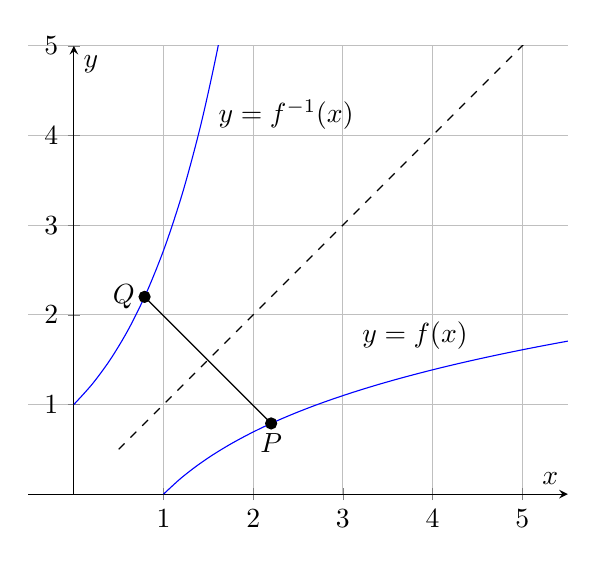
\begin{tikzpicture}
		\begin{axis}[
			xmin=0,xmax=5,
			ymin=0,ymax=5,
			restrict y to domain=0:10,
			grid=both,
			axis equal=true,
			axis lines=middle,
			xlabel=$x$,
			ylabel=$y$,
			axis lines=middle,
		]
			\begin{scope}[color=blue,samples=50,smooth]
				\addplot[domain=0:10]{exp(x)};
				\addplot[domain=1:10]{ln(x)};
			\end{scope}
			\addplot[color=black,dashed,domain=.5:8]{x};
			\filldraw(2.2,{ln(2.2)})circle(2pt)node[below]{$P$}
				--({ln(2.2)},2.2)circle(2pt)node[left]{$Q$};
			\draw(4.5,{ln(4.5)})node[above left]{$y=f(x)$}
				({ln(4.5)},4.5)node[below right]{$y=f^{-1}(x)$};
		\end{axis}
	\end{tikzpicture}
	\caption{}\label{figure:函数.直接函数与反函数的图形的对称性}
\end{figure}

\subsection{复合函数}
\begin{definition}
设函数\(y=f(u)\)的定义域为\(D_f\),
函数\(u=g(x)\)的定义域为\(D_g\),
且其值域\(R_g \subseteq D_f\),
则函数\[
	y = f[g(x)],
	\quad x \in D_g
\]
称为由函数\(u=g(x)\)与函数\(y=f(u)\)构成的\DefineConcept{复合函数},
它的定义域为\(D_g\),变量\(u\)称为\DefineConcept{中间变量}.

函数\(g\)与函数\(f\)构成的复合函数,
即按“先\(g\)后\(f\)”的次序复合的函数,
通常记为\(f \circ g\),即\[
	(f \circ g)(x) = f[g(x)].
\]
\end{definition}

\section{绝对值函数}
\begin{definition}[绝对值]
设\(x \in \mathbb{R}\),则称函数\[
	f(x) = \left\{ \begin{array}{c}
		x, \quad x \geq 0 \\
		-x, \quad x < 0
	\end{array} \right.
\]为\(x\)的绝对值,
记作\(\abs{x}\).
\end{definition}

\begin{figure}[htb]
	\centering
	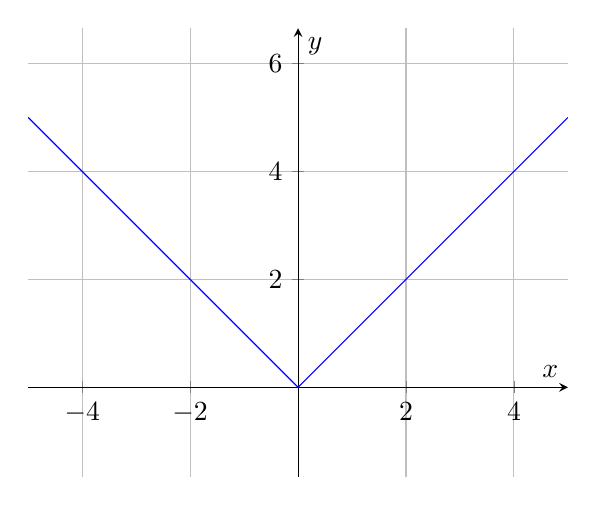
\begin{tikzpicture}
		\begin{axis}[
			xmin=-5,xmax=5,
			ymin=0,ymax=5,
			grid=both,
			axis lines=middle,
			xlabel=$x$,
			ylabel=$y$,
			axis equal=true,
		]
			\addplot[color=blue,samples at={-5,0,5}]{abs(x)};
		\end{axis}
	\end{tikzpicture}
	\caption{绝对值函数\(\abs{x}\)的图形}
\end{figure}

\begin{proposition}
设\(a,b\in\mathbb{R}\),
则\begin{itemize}
	\item \(\abs{a}\geq0\),
	\item \(\abs{a} = \abs{-a}\),
	\item \(\abs{ab} = \abs{a} \abs{b}\),
	\item \(\abs{\frac{a}{b}} = \frac{\abs{a}}{\abs{b}}\ (b\neq0)\),
	\item \(\abs{a}^2 = \abs{a^2}\).
\end{itemize}
\begin{proof}
当\(a=0\)或\(b=0\)时,易见\(\abs{ab} = 0 = \abs{a} \abs{b}\).
当\(a\neq0\)且\(b\neq0\)时,
按照\(a\)和\(b\)的不同取值,列表如下:
\begin{center}
	\begin{tblr}{|*2c|*2{c|}}
		\hline
		&& \(b>0\) & \(b<0\) \\
		&& \(\abs{b}=b\) & \(\abs{b}=-b\) \\ \hline
		\(a>0\) & \(\abs{a}=a\) & \(ab>0,\abs{ab}=ab\) & \(ab<0,\abs{ab}=-ab\) \\ \hline
		\(a<0\) & \(\abs{a}=-a\) & \(ab<0,\abs{ab}=-ab\) & \(ab>0,\abs{ab}=ab\) \\ \hline
	\end{tblr}
\end{center}
由此可知\(\abs{ab} = \abs{a} \abs{b}\)恒成立.
\end{proof}
\end{proposition}

\begin{proposition}
设\(a\)和\(b\)都是实数,
则\begin{gather}
	\min\{a,b\}
	= \frac{a+b}{2}
	- \frac{\abs{a-b}}{2}, \\
	\max\{a,b\}
	= \frac{a+b}{2}
	+ \frac{\abs{a-b}}{2}.
\end{gather}
\begin{proof}
当\(a>b\)时,有\[
	\frac{a+b}{2} - \frac{\abs{a-b}}{2}
	= \frac{a+b}{2} - \frac{a-b}{2}
	= \frac{2b}{2} = b
	= \min\{a,b\},
\]\[
	\frac{a+b}{2} + \frac{\abs{a-b}}{2}
	= \frac{a+b}{2} + \frac{a-b}{2}
	= \frac{2a}{2} = a
	= \max\{a,b\}.
\]
当\(a \leq b\)时,有\[
	\frac{a+b}{2} - \frac{\abs{a-b}}{2}
	= \frac{a+b}{2} - \frac{b-a}{2}
	= \frac{2a}{2} = a
	= \min\{a,b\},
\]\[
	\frac{a+b}{2} + \frac{\abs{a-b}}{2}
	= \frac{a+b}{2} + \frac{b-a}{2}
	= \frac{2b}{2} = b
	= \max\{a,b\}.
	\qedhere
\]
\end{proof}
\end{proposition}

\section{符号函数}
\begin{definition}[符号函数]
函数\[
	f(x) = \left\{ \begin{array}{cc}
		1, & x > 0 \\
		0, & x = 0 \\
		-1, & x < 0 \\
	\end{array} \right.
\]称为\DefineConcept{符号函数},
记作\(\sgn x\).
\end{definition}

\begin{figure}[htb]
	\centering
	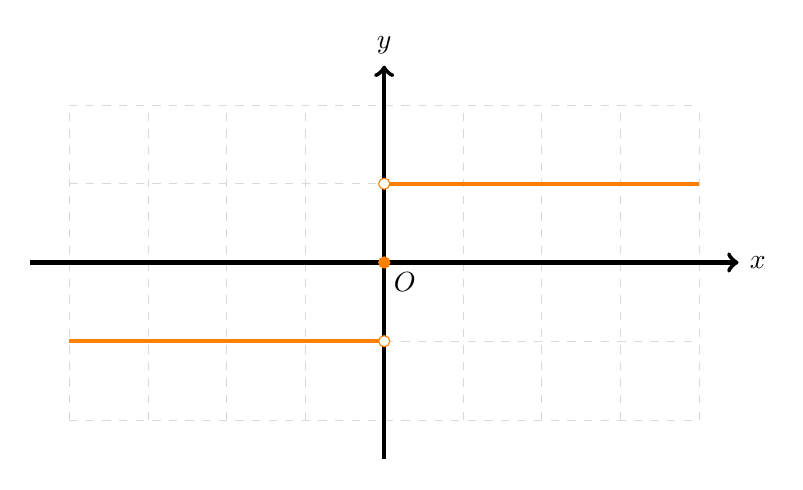
\begin{tikzpicture}
		\draw[help lines, color=gray!30, dashed] (-4,-2) grid (4,2);
		\draw[->, ultra thick] (-4.5,0) -- (4.5,0) node[right]{\(x\)};
		\draw[->, ultra thick] (0,-2.5) -- (0,2.5) node[above]{\(y\)};
		\draw (0,0)node[below right]{\(O\)};
		\draw[orange,ultra thick] (-4,-1)--(0,-1) (0,1)--(4,1);
		\draw[draw=orange,fill=orange] (0,0)circle(2pt);
		\draw[draw=orange,fill=white] (0,1)circle(2pt) (0,-1)circle(2pt);
	\end{tikzpicture}
	\caption{符号函数\(\sgn x\)的图形}
\end{figure}

\section{取整函数}
\begin{definition}[取整函数]
设\(x\in\mathbb{R},
n\in\mathbb{Z}\),定义:
\begin{enumerate}
	\item 如果\(n\)是不大于\(x\)的最大整数,
	即\(x\in[n,n+1)\),
	那么记\(\floor{x}=n\).
	我们把函数\(y=\floor{x}\)称为\DefineConcept{向下取整函数},
	即\begin{equation}
		\floor{x}
		\defeq
		\max\Set{ n\in\mathbb{Z} \given n \leq x }.
	\end{equation}

	\item 如果\(n\)是不小于\(x\)的最小整数,
	即\(x\in(n-1,n]\),
	那么记\(\ceil{x}=n\).
	我们把函数\(y=\ceil{x}\)称为\DefineConcept{向上取整函数},
	即\begin{equation}
		\ceil{x}
		\defeq
		\min\Set{ n\in\mathbb{Z} \given n \geq x }.
	\end{equation}
\end{enumerate}
\end{definition}

\begin{figure}[ht]
	\def\subwidth{.45\linewidth}
	\def\subscale{.9}
	\begin{subfigure}[b]{\subwidth}%
		\centering
		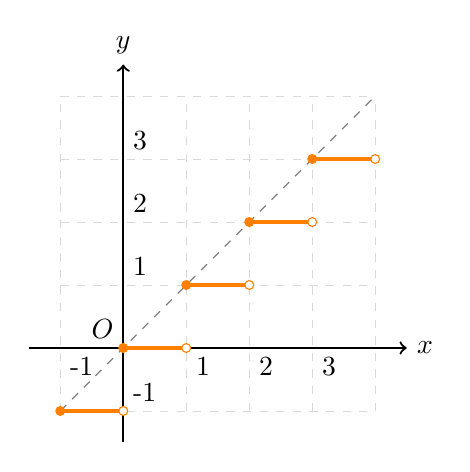
\begin{tikzpicture}[scale=\subscale]
			\tikzstyle{sx}=[draw=orange,fill=orange]
			\tikzstyle{kx}=[draw=orange,fill=white]
			\draw[help lines, color=gray!30, dashed] (-1,-1) grid (4,4);
			\draw[dashed, color=gray] (-1,-1) -- (4,4);
			\draw[->, thick] (-1.5,0) -- (4.5,0) node[right]{\(x\)};
			\draw[->, thick] (0,-1.5) -- (0,4.5) node[above]{\(y\)};
			\foreach \i in {-1,...,3} {
				\draw[ultra thick,orange] (\i,\i)--(\i+1,\i);
				\fill[sx] (\i,\i)circle(2pt);
				\fill[kx] (\i+1,\i)circle(2pt);
				\ifnum\i=0\relax\else
					\draw(\i,0)node[below right]{\i};
					\draw(0,\i)node[above right]{\i};
				\fi
			}
			\draw (0,0)node[above left]{\(O\)};
		\end{tikzpicture}
		\subcaption{向下取整函数\(\floor{x}\)}
	\end{subfigure}
	\begin{subfigure}[b]{\subwidth}%
		\centering
		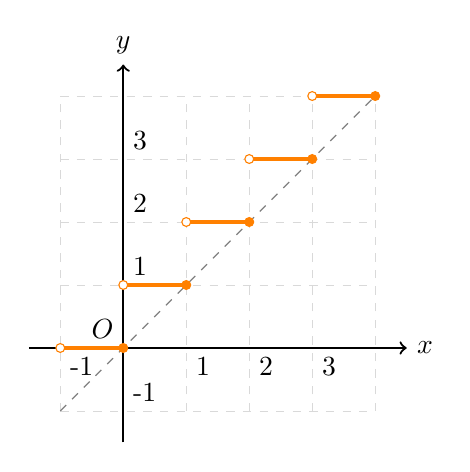
\begin{tikzpicture}[scale=\subscale]
			\tikzstyle{sx}=[draw=orange,fill=orange]
			\tikzstyle{kx}=[draw=orange,fill=white]
			\draw[help lines, color=gray!30, dashed] (-1,-1) grid (4,4);
			\draw[dashed, color=gray] (-1,-1) -- (4,4);
			\draw[->, thick] (-1.5,0) -- (4.5,0) node[right]{\(x\)};
			\draw[->, thick] (0,-1.5) -- (0,4.5) node[above]{\(y\)};
			\foreach \i in {-1,...,3} {
				\draw[ultra thick,orange] (\i,\i+1)--(\i+1,\i+1);
				\fill[kx] (\i,\i+1)circle(2pt);
				\fill[sx] (\i+1,\i+1)circle(2pt);
				\ifnum\i=0\relax\else
					\draw(\i,0)node[below right]{\i};
					\draw(0,\i)node[above right]{\i};
				\fi
			}
			\draw (0,0)node[above left]{\(O\)};
		\end{tikzpicture}
		\subcaption{向上取整函数\(\ceil{x}\)}
	\end{subfigure}
	\caption{取整函数的图形}
\end{figure}

\begin{property}\label{theorem:取整函数.性质1}
一般地,对于\(x\in\mathbb{R}\),总有\begin{equation}
	x - 1 < \floor{x} \leq x \leq \ceil{x} < x + 1.
\end{equation}
\end{property}

\begin{property}
对于\(n\in\mathbb{Z}\),总有\begin{equation}
	\ceil{n/2} + \floor{n/2} = n.
\end{equation}
\end{property}

\begin{property}
对于任意实数\(x \geq 0\)和整数\(a,b>0\),总有\begin{gather}
	\ceil*{\frac{\ceil{x/a}}{b}} = \ceil*{\frac{x}{ab}}, \\
	\floor*{\frac{\floor{x/a}}{b}} = \floor*{\frac{x}{ab}}, \\
	\ceil*{\frac{a}{b}} \leq \frac{a+(b-1)}{b}, \\
	\floor*{\frac{a}{b}} \geq \frac{a-(b-1)}{b}.
\end{gather}
\end{property}

\section{幂函数、指数函数、对数函数}
\begin{definition}
同一个数\(a\ (a\in\mathbb{R})\)连续相乘\(b\ (b\in\mathbb{N})\)次所得的乘积,
称作“\(a\)的\(b\)次方”
或“\(a\)的\(b\)次幂”,
记作\(a^b\),
即\[
	a^b
	\defeq
	\underbrace{a \times a \times \dotsm \times a}_{b\text{次}} = \prod_{i=1}^b a.
\]

特别地,规定:\begin{gather*}
	a^0 \defeq 1 \quad(a\neq0), \\
	a^{-1} \defeq \frac1a \quad(a\neq0), \\
	a^{-n} \defeq \frac1{a^n} \quad(a\neq0), \\
	a^{1/n} \defeq \sqrt[n]{a} \quad(a\geq0). \\
\end{gather*}
\end{definition}

\begin{figure}[ht]
	\centering
	\begin{tikzpicture}
		\def\r{\textcolor{orange}}
		\def\b{\textcolor{blue}}
		\def\p{\textcolor{purple}}
		\draw(0,0)node{\(\r{a}^{\b{b}} = \p{c} \defiff \log_{\r{a}} \p{c} = \b{b}\)};
		\draw(-2.2,-.5)node{\r{底数}}
			(-2.2,.5)node{\b{指数}}
			(-1,-.5)node{\p{幂}}
			(.3,-.5)node{\r{底数}}
			(1.4,-.5)node{\p{真数}}
			(2.3,.5)node{\b{对数}};
		\draw[->](-1.7,-.3)--(-1.7,-1)--(.84,-1)->(.84,-.3); %a
		\draw[->](-1.55,.3)--(-1.55,1)--(1.7,1)->(1.7,.3); %b
		\draw[->](-.86,.3)--(-.86,.7)--(1.1,.7)->(1.1,.3); %c
	\end{tikzpicture}
	\caption{底数、指数、幂与对数的联系}\label{figure:函数.底数、指数、幂与对数的联系}
\end{figure}

\begin{proposition}
\(1\)的任意次幂还是\(1\),即\(1^n = 1\).
\end{proposition}

\begin{proposition}
\(0\)的任意非零次幂还是\(0\),即\(0^n = 0\ (n\neq0)\).
\end{proposition}

\subsection{幂函数的概念}
\begin{definition}[幂函数]
函数\(f(x)=x^{\mu}\ (\mu \in \mathbb{R})\),
称为\DefineConcept{幂函数}.
\end{definition}

\subsection{幂函数的性质}
\begin{property}
幂函数具有以下性质:
\begin{itemize}
	\item 当\(\mu = 0\)时,
	幂函数\(f(x)=x^{\mu}\)在定义域\((-\infty,+\infty)\)上恒为一,
	是常数函数.

	\item 当\(\mu\)为正奇数时,
	幂函数\(f(x)=x^{\mu}\)为奇函数,
	其定义域、值域均为\((-\infty,+\infty)\),它在定义域内恒单调递增.

	\item 当\(\mu\)为正偶数时,
	幂函数\(f(x)=x^{\mu}\)为偶函数,
	其定义域为\((-\infty,+\infty)\),其值域为\([0,+\infty)\),
	它在\((-\infty,0]\)上单调递减,在\([0,+\infty)\)上单调递增.

	\item 当\(\mu\)为负奇数时,
	幂级数\(y=x^{\mu}\)又称为\DefineConcept{比例函数},
	其定义域、值域为\((-\infty,0)\cup(0,+\infty)\),
	它在区间\((-\infty,0)\)和\((0,+\infty)\)内单调递减.

	若幂函数前有常系数大于零则称之为\DefineConcept{正比例函数}.
	%@Mathematica: Plot[Evaluate[x^-n /. n -> {1, 2, 3, 4, 5}], {x, 0, 2}, PlotRange -> {0, 2}, PlotLegends -> Automatic]

	若幂函数前有常系数小于零则称之为\DefineConcept{反比例函数}.
	%@Mathematica: Plot[Evaluate[x^-n /. n -> {1, 2, 3, 4, 5}], {x, -2, 0}, PlotRange -> {-2, 2}, PlotLegends -> Automatic]

	\item 当\(\mu\)为负偶数时,
	幂函数\(f(x)=x^{\mu}\)为偶函数,
	其定义域为\((-\infty,0)\cup(0,+\infty)\),其值域为\((0,+\infty)\),
	它在\((-\infty,0)\)内单调递增,在\((0,+\infty)\)内单调递减.

	\item 当\(\mu = \pm\frac{m}{n} \in \mathbb{Q}\)(\(m,n>0\)且\(m\)、\(n\)是互质的整数)时,
	幂函数\(f(x)=x^{\mu}=x^{\pm\frac{m}{n}}\)可改写为\(y=\sqrt[n]{x^m}\)(\(\mu>0\)时)
	或\(y=\frac{1}{\sqrt[n]{x^m}}\)(\(\mu<0\)时).
\end{itemize}
\end{property}

\begin{figure}[ht]
	\centering
	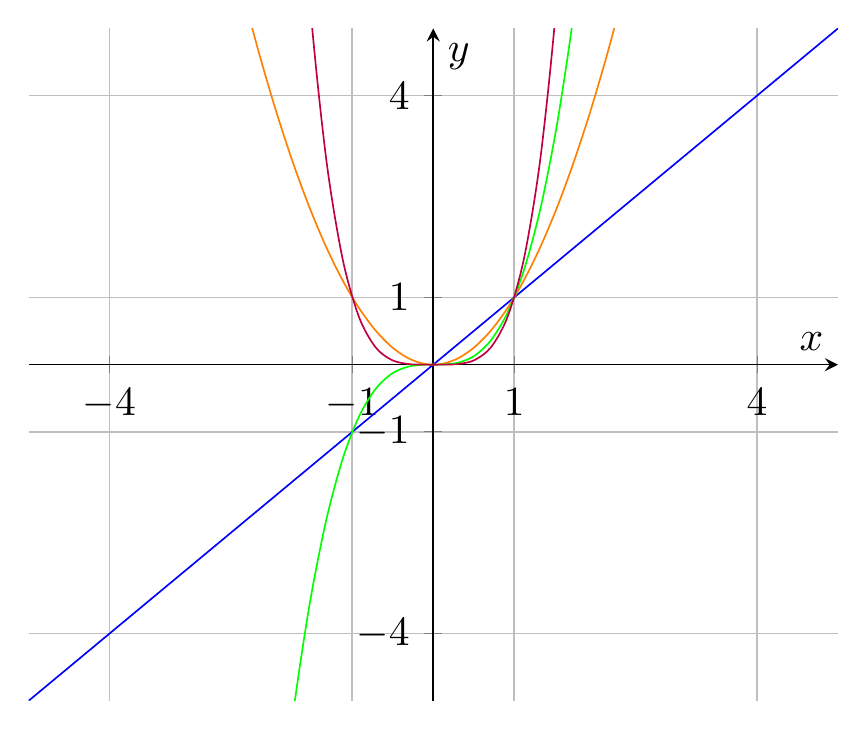
\begin{tikzpicture}[scale=1.5]
		\begin{axis}[
			xmin=-5,xmax=5,
			ymin=-5,ymax=5,
			enlargelimits,
			axis lines=middle,
			xlabel=$x$,
			ylabel=$y$,
			xtick={-4,-1,1,4},
			ytick={-4,-1,1,4},
			grid=major,
		]
			\begin{scope}[samples=50,smooth,domain=-5:5]
				\addplot[color=blue]{x};
				\addplot[color=orange]{x^2};
				\addplot[color=green]{x^3};
				\addplot[color=purple]{x^4};
			\end{scope}
		\end{axis}
	\end{tikzpicture}
	\caption{}
\end{figure}

\begin{figure}
	\centering
	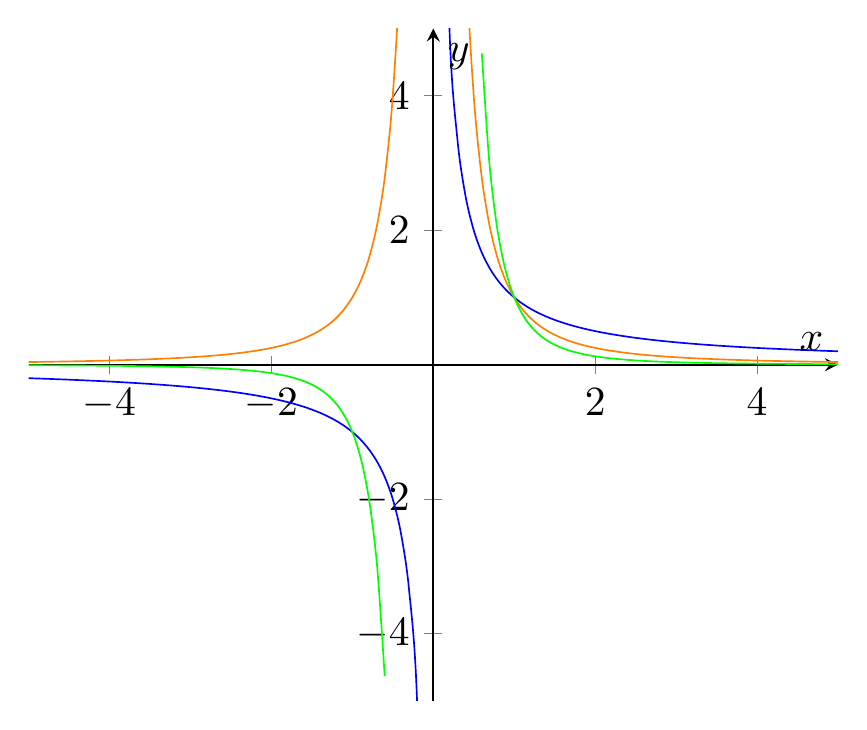
\begin{tikzpicture}[scale=1.5]
		\begin{axis}[
			xmin=-5,xmax=5,
			ymin=-5,ymax=5,
			enlargelimits,
			axis lines=middle,
			xlabel=$x$,
			ylabel=$y$,
		]
			\begin{scope}[samples=50,smooth]
				\begin{scope}[domain=-5:-.1]
					\addplot[color=blue]{1/x};
					\addplot[color=orange]{1/(x^2)};
					\addplot[color=green,domain=-5:-.6]{1/(x^3)};
				\end{scope}
				\begin{scope}[domain=.1:5]
					\addplot[color=blue]{1/x};
					\addplot[color=orange]{1/(x^2)};
					\addplot[color=green,domain=.6:5]{1/(x^3)};
				\end{scope}
			\end{scope}
		\end{axis}
	\end{tikzpicture}
	\caption{}
\end{figure}

\subsection{指数函数的概念}
\begin{definition}
设\(a>0\)且\(a \neq 1\).
把函数\(f(x)=a^x\)
称为“以\(a\)为底的\DefineConcept{指数函数}”.
\end{definition}

\begin{theorem}
设\(f\)是以\(a\)为底的指数函数,
则\(f\)存在反函数.
\begin{proof}
指数函数是单调函数.
\end{proof}
\end{theorem}

\subsection{对数函数的概念}
\begin{definition}
以\(a\)为底的指数函数的反函数,
称为“以\(a\)为底的\DefineConcept{对数函数}”,
记作\(y=\log_a x\).

特别地,以\(10\)为底的对数,称为\DefineConcept{常用对数},记作\(y = \lg x\);
以常数\(e\)为底的对数,称为\DefineConcept{自然对数},记作\(y = \ln x\).
%@see: https://mathworld.wolfram.com/Logarithm.html
\end{definition}

\subsection{指数函数、对数函数的性质}
\begin{proposition}[对数恒等式]
设\(a>0\)且\(a\neq1\),
则对\(\forall x>0\)
有\begin{gather}
	a^{\log_a x} = x.
\end{gather}
\end{proposition}

\begin{corollary}
设\(a>0\)且\(a\neq1\),
则\begin{equation}
	\log_a a^x = x.
\end{equation}
\end{corollary}

\begin{theorem}[换底公式]
设\(a>0,a\neq1,c>0,c\neq1,b>0\),
则\begin{equation}\label{equation:函数.换底公式}
	\log_a b = \frac{\log_c b}{\log_c a}.
\end{equation}
\end{theorem}

\begin{corollary}
设\(a>0,a\neq1,b>0,b\neq1\),
则\begin{equation}
	\log_a b = \frac1{\log_b a}.
\end{equation}
\end{corollary}

\begin{property}
\begin{gather}
	a^x a^y = a^{x+y}, \\
	\frac{a^x}{a^y} = a^{x-y}, \\
	(a^x)^y = a^{xy}.
\end{gather}
\end{property}

\begin{property}
设\(a>0\)且\(a\neq1\),
则\begin{gather}
	\log_a xy = \log_a x + \log_a y, \\
	\log_a \frac{x}{y} = \log_a x - \log_a y, \\
	\log_a x^y = y \log_a x.
\end{gather}
\end{property}

\begin{corollary}
若\(a,a^x \in (0,1)\cup(1,+\infty)\),
则\[
	\log_{a^x} b^y = \frac{y}{x} \log_a b.
\]
\end{corollary}

\begin{example}
证明:\begin{equation}\label{equation:函数.真底互换公式}
	a^{\ln b} = b^{\ln a}.
\end{equation}
\begin{proof}
在\cref{equation:函数.真底互换公式} 等号左右变量分别取对数,
得\[
	\ln(a^{\ln b}) = \ln b \ln a, \qquad
	\ln(b^{\ln a}) = \ln a \ln b,
\]
显然两者相等,故\(a^{\ln b} = b^{\ln a}\)成立.
\end{proof}
\end{example}

\subsection{重幂}
设\(a\)是实数,\(b\)是正整数.
定义:\[
	\relax^ba \defeq \underbrace{a^{a^{\iddots^a}}}_{\text{\(b\)个}},
\]
我们把\(\relax^ba\)读作“\(a\)的\(b\)~\DefineConcept{重幂}”.

例如,\[
	\relax^23 = 3^3, \qquad
	\relax^33 = 3^{3^3}, \qquad
	\relax^43 = 3^{3^{3^3}}.
\]

\section{三角函数}
\subsection{三角函数的概念}
\begin{figure}[ht]
	\centering
	\begin{tikzpicture}
		\draw[help lines, color=gray!30, dashed](0,0)grid(4,3);
		\coordinate(A)at(0,0);
		\coordinate(B)at(4,0);
		\coordinate(C)at(4,3);
		\draw (A)node[left]{\(A\)}
			--(B)node[right]{\(B\)}node[midway,below]{\(c\)}
			--(C)node[right]{\(C\)}node[midway,right]{\(a\)}
			--(A)node[midway,left,above]{\(b\)}
			pic["\(\theta\)",draw=orange,-,angle eccentricity=2,angle radius=0.3cm]{angle=B--A--C}
			pic[draw=gray,-,angle radius=0.3cm]{right angle=C--B--A};
	\end{tikzpicture}
	\caption{}
	\label{figure:函数.三角函数.三角函数的几何定义}
\end{figure}

\begin{definition}\label{definition:函数.三角函数的几何定义}
如\cref{figure:函数.三角函数.三角函数的几何定义},
取任意一个直角三角形\(\triangle ABC\),
其中\(\angle B\)是直角(即\(\angle ABC = \pi/2\)),
假设\(\angle BAC = \theta\).
定义三角函数如下:
\begin{center}
	\begin{tabular}{cc|cc|cc}
		\hline
		名称 & 定义式 & 名称 & 定义式 & 名称 & 定义式 \\ \hline
		正弦 & \(\sin\theta = a/b\)
			& 正切 & \(\tan\theta = a/c\)
				& 正割 & \(\sec\theta = b/c\) \\
		余弦 & \(\cos\theta = c/b\)
			& 余切 & \(\cot\theta = c/a\)
				& 余割 & \(\csc\theta = b/a\) \\
		\hline
	\end{tabular}
\end{center}
\end{definition}

\begin{example}
下面列出一些特殊的正弦函数值:\[
\sin0 = 0, \quad
\sin\frac{\pi}{6} = \frac{1}{2}, \quad
\sin\frac{\pi}{4} = \frac{\sqrt{2}}{2}, \quad
\sin\frac{\pi}{3} = \frac{\sqrt{3}}{2},
\]\[
\sin\frac{\pi}{2} = 1, \quad
\sin\pi = 0, \quad
\sin\frac{3\pi}{2} = -1.
\]

\begin{figure}[ht]
	\centering
	\begin{tikzpicture}
		\pgfmathsetmacro{\r}{2}
		\pgfmathsetmacro{\ax}{\r*cos(30)}
		\pgfmathsetmacro{\ay}{\r*sin(30)}
		\pgfmathsetmacro{\b}{\r/sqrt(2)}
		\coordinate (O)at(0,0);
		\draw(O)circle(\r);
		\begin{scope}[dashed,color=gray!50,text=black]
			\draw(O)--(\r,0)node[left]{\(0\)}node[right]{\(0\)}
			(O)--(\ax,\ay)node[below left]{\(\tfrac{\pi}{6}\)}node[right]{\(\tfrac{1}{2}\)}
			(O)--(\b,\b)node[below left]{\(\tfrac{\pi}{4}\)}node[above right]{\(\tfrac{\sqrt2}{2}\)}
			(O)--(\ay,\ax)node[below left]{\(\tfrac{\pi}{3}\)}node[above]{\(\tfrac{\sqrt3}{2}\)}
			(O)--(0,\r)node[below]{\(\tfrac{\pi}{2}\)}node[above]{\(1\)}
			(O)--(-\ay,\ax)node[below right]{\(\tfrac{2\pi}{3}\)}node[above]{\(\tfrac{\sqrt3}{2}\)}
			(O)--(-\b,\b)node[below right]{\(\tfrac{3\pi}{4}\)}node[above left]{\(\tfrac{\sqrt2}{2}\)}
			(O)--(-\ax,\ay)node[below right]{\(\tfrac{5\pi}{6}\)}node[left]{\(\tfrac{1}{2}\)}
			(O)--(-\r,0)node[right]{\(\pi\)}node[left]{\(0\)}
			(O)--(-\ax,-\ay)node[above right]{\(\tfrac{7\pi}{6}\)}node[left]{\(-\tfrac{1}{2}\)}
			(O)--(-\b,-\b)node[above right]{\(\tfrac{5\pi}{4}\)}node[below left]{\(-\tfrac{\sqrt2}{2}\)}
			(O)--(-\ay,-\ax)node[above right]{\(\tfrac{4\pi}{3}\)}node[below]{\(-\tfrac{\sqrt3}{2}\)}
			(O)--(0,-\r)node[above]{\(\tfrac{3\pi}{2}\)}node[below]{\(-1\)}
			(O)--(\ay,-\ax)node[above left]{\(\tfrac{5\pi}{3}\)}node[below]{\(-\tfrac{\sqrt3}{2}\)}
			(O)--(\b,-\b)node[above left]{\(\tfrac{7\pi}{4}\)}node[below right]{\(-\tfrac{\sqrt2}{2}\)}
			(O)--(\ax,-\ay)node[above left]{\(\tfrac{11\pi}{6}\)}node[right]{\(-\tfrac{1}{2}\)}
			;
		\end{scope}
		\begin{scope}[very thick,->]
			\draw(-1,0)--(1,0)node[above left]{\(x\)};
			\draw(0,-1)--(0,1)node[below right]{\(y\)};
		\end{scope}
	\end{tikzpicture}
	\caption{正弦函数\(\sin x\)的辅助圆与特殊值}
\end{figure}

特殊的余弦函数值:\[
	\cos0 = 1, \quad
	\cos\frac{\pi}{6} = \frac{\sqrt{3}}{2}, \quad
	\cos\frac{\pi}{4} = \frac{\sqrt{2}}{2}, \quad
	\cos\frac{\pi}{3} = \frac{1}{2},
\]\[
	\cos\frac{\pi}{2} = 0, \quad
	\cos\pi = -1, \quad
	\cos\frac{3\pi}{2} = 0.
\]
\end{example}

\subsection{三角函数的性质}
\begin{property}
根据三角函数的定义,显然有\begin{gather}
	\cot\theta = \frac{1}{\tan\theta}, \\
	\sec\theta = \frac{1}{\cos\theta}, \\
	\csc\theta = \frac{1}{\sin\theta}.
\end{gather}
\end{property}

\begin{theorem}[毕达哥拉斯三角恒等式]
\begin{figure}[ht]
	\def\subwidth{.5\linewidth}
	\def\subscale{.8}
		\begin{subfigure}[b]{\subwidth}%
		\centering
		\begin{tikzpicture}[scale=\subscale]
			\draw[help lines, color=gray!30, dashed] (0,0) grid (4,3);
			\coordinate (A) at (0,0);
			\coordinate (B) at (4,0);
			\coordinate (C) at (4,3);
			\draw (A)node[left]{\(A\)} -- (B)node[right]{\(B\)}node[midway,below]{\(\cos\theta\)} -- (C)node[right]{\(C\)}node[midway,right]{\(\sin\theta\)} -- (A)node[midway,above left]{\(1\)} pic["\(\theta\)",draw=orange,-,angle eccentricity=2,angle radius=0.3cm]{angle=B--A--C} pic[draw=gray,-,angle radius=0.3cm]{right angle=C--B--A};
		\end{tikzpicture}
		\subcaption{正弦、余弦辅助三角形}
		\end{subfigure}%
		\begin{subfigure}[b]{\subwidth}%
		\centering
		\begin{tikzpicture}[scale=\subscale]
			\draw[help lines, color=gray!30, dashed] (0,0) grid (4,3);
			\coordinate (A) at (0,0);
			\coordinate (B) at (4,0);
			\coordinate (C) at (4,3);
			\draw (A)node[left]{\(A\)} -- (B)node[right]{\(B\)}node[midway,below]{\(1\)} -- (C)node[right]{\(C\)}node[midway,right]{\(\tan\theta\)} -- (A)node[midway,above left]{\(\sec\theta\)} pic["\(\theta\)",draw=orange,-,angle eccentricity=2,angle radius=0.3cm]{angle=B--A--C} pic[draw=gray,-,angle radius=0.3cm]{right angle=C--B--A};
		\end{tikzpicture}
		\subcaption{正切、正割辅助三角形}
		\end{subfigure}%
	\caption{两种特殊的辅助三角形}
	\label{figure:函数.两种特殊的辅助三角形}
\end{figure}

结合\cref{figure:函数.两种特殊的辅助三角形},根据勾股定理可得
\begin{gather}
	\sin^2 \theta + \cos^2 \theta = 1, \\
	\tan^2 \theta + 1 = \sec^2 \theta, \\
	1 + \cot^2 \theta = \csc^2 \theta.
\end{gather}
\end{theorem}

\begin{figure}[ht]
	\centering
	\begin{tikzpicture}
		\pgfmathsetmacro{\a}{6}
		\coordinate(O)at(0,0);
		\pgfmathsetmacro{\t}{30}
		\draw(O)node[below left]{\(O\)}
			--(\a,0)coordinate(A)node[below right]{\(A\)}
			arc[start angle=0,end angle=\t,radius=\a]coordinate(B)node[right]{\(B\)}
			--(O);
		\draw(B)--(B|-A)coordinate(C)node[below right]{\(C\)};
		\draw(B)--(\a,{\a*tan(\t)})coordinate(D)node[above right]{\(D\)}--(\a,0);
		\pic["\(\theta\)",draw,-,angle eccentricity=1.5,angle radius=6mm]{angle=A--O--B};
		\begin{scope}[|<->|,black!40,every node/.style={black,midway,sloped}]
			\def\mark#1#2#3#4#5{%
				\draw($#1+#4$)--($#2+#4$)node[#3]{$#5$};%
			}%
			\mark{(C)}{(B)}{above}{(-5pt,0)}{\sin\theta}
			\mark{(O)}{(D)}{above}{({(-1em-10pt)*sin(30)},{(1em+10pt)*cos(30)})}{\sec\theta}
			\mark{(O)}{(B)}{above}{({-5pt*sin(30)},{5pt*cos(30)})}{1}
			\mark{(O)}{(C)}{below}{(0,-5pt)}{\cos\theta}
			\mark{(A)}{(D)}{below}{(5pt,0)}{\tan\theta}
			\mark{(O)}{(A)}{below}{(0,-1em-10pt)}{1}
		\end{scope}
	\end{tikzpicture}
	\caption{}
\end{figure}

\begin{figure}[ht]
	\centering
	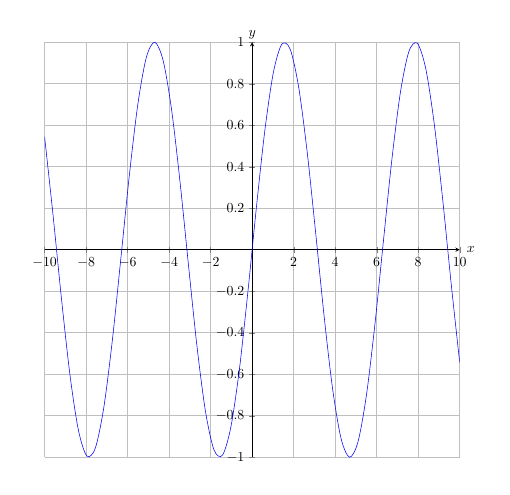
\begin{tikzpicture}[scale=.5]
		\begin{axis}[
			xmin=-10,xmax=10,
			restrict y to domain=-2:2,
			ymin=-1,ymax=1,
			grid=both,width=\textwidth,height=\textwidth,
			axis lines=middle,
			xlabel=$x$,
			ylabel=$y$,
			enlarge x limits=0.1,
			enlarge y limits=0.1,
			axis lines = middle,
			x label style={at={(ticklabel* cs:1.00)}, inner sep=5pt, anchor=west},
			y label style={at={(ticklabel* cs:1.00)}, inner sep=2pt, anchor=south},
		]
			\addplot[color=blue,samples=50,smooth,domain=-10:10,variable=\x]{sin(\x r)};
		\end{axis}
	\end{tikzpicture}
	\caption{正弦函数\(y=\sin x\)的图形}
	\label{figure:函数.正弦函数的图形}
\end{figure}

\begin{figure}
	\centering
	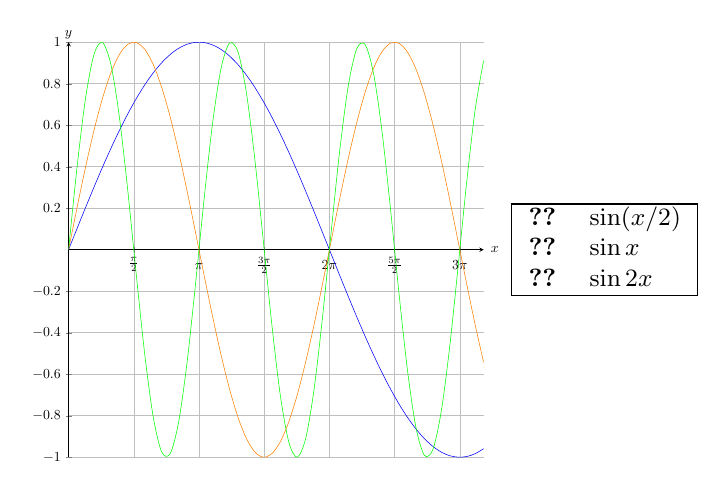
\begin{tikzpicture}[scale=.5]
		\begin{axis}[
			name=Sine,
			xmin=0,xmax=10,
			restrict y to domain=-2:2,
			ymin=-1,ymax=1,
			grid=both,width=\textwidth,height=\textwidth,
			axis lines=middle,
			xlabel=$x$,
			ylabel=$y$,
			axis lines = middle,
			x label style={at={(ticklabel* cs:1.00)}, inner sep=5pt, anchor=west},
			y label style={at={(ticklabel* cs:1.00)}, inner sep=2pt, anchor=south},
			xtick={0,1.5708,3.1416,...,10},
			xticklabels={
				$\relax$,
				$\frac{\pi}{2}$,
				$\pi\vphantom{\frac12}$,
				$\frac{3\pi}{2}$,
				$2\pi\vphantom{\frac12}$,
				$\frac{5\pi}{2}$,
				$3\pi\vphantom{\frac12}$,
			},
		]
			\addplot[color=blue,samples=50,smooth,domain=0:10,variable=\x]
				{sin(.5*\x r)};\label{pgfplots:正弦函数.sin(x/2)}
			\addplot[color=orange,samples=50,smooth,domain=0:10,variable=\x]
				{sin(\x r)};\label{pgfplots:正弦函数.sin(x)}
			\addplot[color=green,samples=50,smooth,domain=0:10,variable=\x]
				{sin(2*\x r)};\label{pgfplots:正弦函数.sin(2*x)}
		\end{axis}
		\node[draw,fill=white,inner sep=0pt,right=1em]at(Sine.east){\small\begin{tabular}{cl}
		\ref{pgfplots:正弦函数.sin(x/2)} & \(\sin(x/2)\) \\
		\ref{pgfplots:正弦函数.sin(x)} & \(\sin x\) \\
		\ref{pgfplots:正弦函数.sin(2*x)} & \(\sin2x\) \\
		\end{tabular}};
	\end{tikzpicture}
	\caption{}
\end{figure}

\begin{property}
如\cref{figure:函数.正弦函数的图形},
可以观察得出正弦函数的若干性质.
\begin{enumerate}
	\item 正弦函数是周期函数,其周期为\(T = 2\pi\).
	\item 正弦函数在区间\([2k\pi-\frac{\pi}{2},2k\pi+\frac{\pi}{2})\)上单调递增.
	\item 在区间\([2k\pi+\frac{\pi}{2},2k\pi+\frac{3\pi}{2})\)上单调递增.
	\item 当\(x=\frac{\pi}{2}+2k\pi\ (k\in\mathbb{Z})\)时,正弦函数\(y=\sin x\)取得极大值\(1\).
	\item 当\(x=\frac{3\pi}{2}+2k\pi\ (k\in\mathbb{Z})\)时,正弦函数\(y=\sin x\)取得极小值\(-1\).
	\item 正弦函数是奇函数,其图形关于坐标原点\(O\)中心对称,满足\(\sin(-x)=-\sin x\).
\end{enumerate}
\end{property}

\begin{figure}[ht]
	\centering
	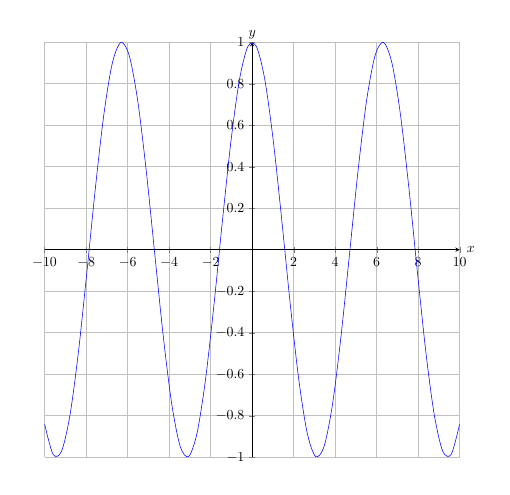
\begin{tikzpicture}[scale=.5]
		\begin{axis}[
			xmin=-10,xmax=10,
			restrict y to domain=-2:2,
			ymin=-1,ymax=1,
			grid=both,width=\textwidth,height=\textwidth,
			axis lines=middle,
			xlabel=$x$,
			ylabel=$y$,
			enlarge x limits=0.1,
			enlarge y limits=0.1,
			axis lines = middle,
			x label style={at={(ticklabel* cs:1.00)}, inner sep=5pt, anchor=west},
			y label style={at={(ticklabel* cs:1.00)}, inner sep=2pt, anchor=south},
		]
			\addplot[color=blue,samples=50,smooth,domain=-10:10,variable=\x]{cos(\x r)};
		\end{axis}
	\end{tikzpicture}
	\caption{余弦函数\(y=\cos x\)的图形}
	\label{figure:函数.余弦函数的图形}
\end{figure}

\begin{figure}
	\centering
	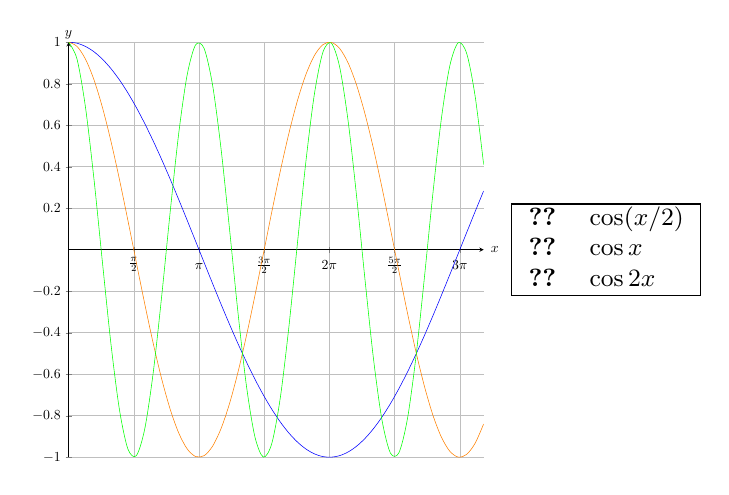
\begin{tikzpicture}[scale=.5]
		\begin{axis}[
			name=Cosine,
			xmin=0,xmax=10,
			restrict y to domain=-2:2,
			ymin=-1,ymax=1,
			grid=both,width=\textwidth,height=\textwidth,
			axis lines=middle,
			xlabel=$x$,
			ylabel=$y$,
			axis lines = middle,
			x label style={at={(ticklabel* cs:1.00)}, inner sep=5pt, anchor=west},
			y label style={at={(ticklabel* cs:1.00)}, inner sep=2pt, anchor=south},
			xtick={0,1.5708,3.1416,...,10},
			xticklabels={
				$\relax$,
				$\frac{\pi}{2}$,
				$\pi\vphantom{\frac12}$,
				$\frac{3\pi}{2}$,
				$2\pi\vphantom{\frac12}$,
				$\frac{5\pi}{2}$,
				$3\pi\vphantom{\frac12}$,
			},
		]
			\addplot[color=blue,samples=50,smooth,domain=0:10,variable=\x]
				{cos(.5*\x r)};\label{pgfplots:余弦函数.cos(x/2)}
			\addplot[color=orange,samples=50,smooth,domain=0:10,variable=\x]
				{cos(\x r)};\label{pgfplots:余弦函数.cos(x)}
			\addplot[color=green,samples=50,smooth,domain=0:10,variable=\x]
				{cos(2*\x r)};\label{pgfplots:余弦函数.cos(2*x)}
		\end{axis}
		\node[draw,fill=white,inner sep=0pt,right=1em]at(Cosine.east){\small\begin{tabular}{cl}
		\ref{pgfplots:余弦函数.cos(x/2)} & \(\cos(x/2)\) \\
		\ref{pgfplots:余弦函数.cos(x)} & \(\cos x\) \\
		\ref{pgfplots:余弦函数.cos(2*x)} & \(\cos2x\) \\
		\end{tabular}};
	\end{tikzpicture}
	\caption{}
\end{figure}

\begin{property}
如\cref{figure:函数.余弦函数的图形},
可以观察得出余弦函数的若干性质.
\begin{enumerate}
	\item 余弦函数也是周期函数,其周期为\(T = 2\pi\).
	\item 余弦函数在区间\([2k\pi,\pi+2k\pi)\)上单调递减.
	\item 在区间\([\pi+2k\pi,2\pi+2k\pi)\)上单调递增.
	\item 当\(x=2k\pi\ (k\in\mathbb{Z})\)时,余弦函数\(y=\cos x\)取得极大值\(1\).
	\item 当\(x=(2k-1)\pi\ (k\in\mathbb{Z})\)时,余弦函数\(y=\cos x\)取得极小值\(-1\).
	\item 余弦函数是偶函数,其图形关于\(y\)轴对称,满足\(\cos(-x)=\cos x\).
\end{enumerate}
\end{property}

\begin{figure}[ht]
	\centering
	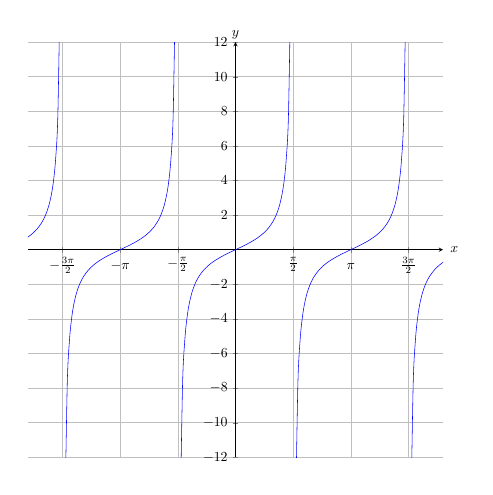
\begin{tikzpicture}[scale=.5]
		\begin{axis}[
			restrict y to domain=-20:20,
			ymin=-10,ymax=10,
			grid=both,width=\textwidth,height=\textwidth,
			axis lines=middle,
			xlabel=$x$,
			ylabel=$y$,
			enlarge x limits=0.1,
			enlarge y limits=0.1,
			x label style={at={(ticklabel* cs:1.00)}, inner sep=5pt, anchor=west},
			y label style={at={(ticklabel* cs:1.00)}, inner sep=2pt, anchor=south},
			xmin=-4.7124, xmax=4.7124,
			xtick={-4.7124,-3.1416,-1.5708,...,10},
			xticklabels={
				$-\frac{3\pi}{2}$,
				$-\pi\vphantom{\frac{1}{2}}$,
				$-\frac{\pi}{2}$,
				$\relax$,%不能去掉\relax
				$\frac{\pi}{2}$,
				$\pi\vphantom{\frac{1}{2}}$,
				$\frac{3\pi}{2}$,
			},
		]
			\foreach \i in {-5,-3,...,3} {
				\addplot[color=blue,samples=50,smooth,domain={\i*pi/2}:{(\i+2)*pi/2},variable=\x]
				{tan(\x r)};
			}
		\end{axis}
	\end{tikzpicture}
	\caption{正切函数\(y=\tan x\)的图形}
	\label{figure:函数.正切函数的图形}
\end{figure}

\begin{property}
如\cref{figure:函数.正切函数的图形},
可以观察得出正切函数的若干性质.
\begin{enumerate}
	\item 正切函数是周期函数,其周期为\(T = \pi\).
	\item 正切函数在区间\((k\pi-\frac{\pi}{2},k\pi+\frac{\pi}{2})\ (k\in\mathbb{Z})\)上单调递增.
	\item 正切函数是奇函数,其图形关于坐标原点\(O\)中心对称,满足\(\tan(-x)=-\tan x\).
\end{enumerate}
\end{property}

\begin{figure}[ht]
	\centering
	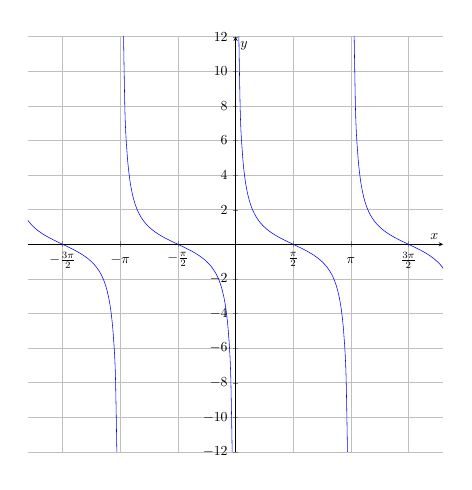
\begin{tikzpicture}[scale=.5]
		\begin{axis}[
			restrict y to domain=-20:20,
			ymin=-10,ymax=10,
			grid=both,width=\textwidth,height=\textwidth,
			axis lines=middle,
			xlabel=$x$,
			ylabel=$y$,
			enlarge x limits=0.1,
			enlarge y limits=0.1,
			xmin=-4.7124, xmax=4.7124,
			xtick={-4.7124,-3.1416,-1.5708,...,10},
			xticklabels={
				$-\frac{3\pi}{2}$,
				$-\pi\vphantom{\frac{1}{2}}$,
				$-\frac{\pi}{2}$,
				$\relax$,%不能去掉\relax
				$\frac{\pi}{2}$,
				$\pi\vphantom{\frac{1}{2}}$,
				$\frac{3\pi}{2}$,
			},
		]
		\foreach \i in {-2,-1,0,1} {
			\addplot[color=blue,samples=50,smooth,domain={\i*pi}:{(\i+1)*pi},variable=\x]
			{cot(\x r)};
		}
		\end{axis}
	\end{tikzpicture}
	\caption{余切函数\(y=\cot x\)的图形}
\end{figure}

\subsection{和积互化公式}
\begin{theorem}[和积互化公式]
\begin{gather}
	\sin(\alpha\pm\beta) = \sin\alpha\cos\beta\pm\cos\alpha\sin\beta,
	\label{equation:函数.三角函数.和积互化公式1} \\
	\cos(\alpha\pm\beta) = \cos\alpha\cos\beta\mp\sin\alpha\sin\beta,
	\label{equation:函数.三角函数.和积互化公式2} \\
	\tan(\alpha\pm\beta) = \frac{\tan\alpha\pm\tan\beta}{1\mp\tan\alpha\tan\beta},
	\label{equation:函数.三角函数.和积互化公式3} \\
	\cot(\alpha\pm\beta) = \frac{\cot\alpha\cot\beta\mp 1}{\cot\beta\pm\cot\alpha},
	\label{equation:函数.三角函数.和积互化公式4} \\
	\sec(\alpha\pm\beta) = \frac{\sec\alpha\sec\beta}{1\mp\tan\alpha\tan\beta},
	\label{equation:函数.三角函数.和积互化公式5} \\
	\csc(\alpha\pm\beta) = \frac{\csc\alpha\csc\beta}{\cot\beta\pm\cot\alpha},
	\label{equation:函数.三角函数.和积互化公式6} \\
	\sin \alpha \cos \beta = \frac{\sin (\alpha + \beta) + \sin (\alpha - \beta)}{2},
	\label{equation:函数.三角函数.和积互化公式7} \\
	\cos \alpha \sin \beta = \frac{\sin (\alpha + \beta) - \sin (\alpha - \beta)}{2},
	\label{equation:函数.三角函数.和积互化公式8} \\
	\cos \alpha \cos \beta = \frac{\cos (\alpha + \beta) + \cos (\alpha - \beta)}{2},
	\label{equation:函数.三角函数.和积互化公式9} \\
	\sin \alpha \sin \beta = -\frac{\cos (\alpha + \beta) - \cos (\alpha - \beta)}{2},
	\label{equation:函数.三角函数.和积互化公式10} \\
	\sin \alpha + \sin \beta = 2 \sin \frac{\alpha + \beta}{2} \cos \frac{\alpha - \beta}{2},
	\label{equation:函数.三角函数.和积互化公式11} \\
	\sin \alpha - \sin \beta = 2 \cos \frac{\alpha + \beta}{2} \sin \frac{\alpha - \beta}{2},
	\label{equation:函数.三角函数.和积互化公式12} \\
	\cos \alpha + \cos \beta = 2 \cos \frac{\alpha + \beta}{2} \cos \frac{\alpha - \beta}{2},
	\label{equation:函数.三角函数.和积互化公式13} \\
	\cos \alpha - \cos \beta = -2 \sin \frac{\alpha + \beta}{2} \sin \frac{\alpha - \beta}{2}.
	\label{equation:函数.三角函数.和积互化公式14}
\end{gather}
\begin{proof}
\begin{figure}[ht]
	\centering
	\begin{tikzpicture}
		\coordinate(A)at(0.0,0.0);
		\coordinate(B)at(6.4,0.0);
		\coordinate(C)at(6.4,4.8);
		\coordinate(D)at(6.4,6.4);
		\coordinate(E)at(5.2,6.4);
		\draw (A)
			--(B)node[midway,below]{\(\cos\alpha\cos\beta\)}
			--(C)node[midway,right]{\rotatebox{90}{\(\cos\alpha\sin\beta\)}}
			--(D)node[midway,right]{\rotatebox{90}{\(\sin\alpha\cos\beta\)}}
			--(E)node[midway,above]{\(\sin\alpha\sin\beta\)}
			--(C)node[midway,left=2mm,below=-3mm]{\rotatebox{-53.13}{\(\sin\alpha\)}}
			--(A)node[midway,right=1mm,below=-2mm]{\rotatebox{36.87}{\(\cos\alpha\)}}
			--(E)node[midway,left=2mm,above=2mm]{\(1\)};
		\pic["\(\alpha\)",draw=orange,-,angle eccentricity=2,angle radius=0.7cm]{angle=C--A--E};
		\pic["\(\beta\)",draw=blue,-,angle eccentricity=2,angle radius=0.7cm]{angle=B--A--C};
		\pic[draw=blue,-,angle radius=0.5cm]{angle=D--C--E};
		\pic[draw=gray,-,angle radius=0.3cm]{right angle=C--B--A};
		\pic[draw=gray,-,angle radius=0.3cm]{right angle=E--C--A};
		\pic[draw=gray,-,angle radius=0.3cm]{right angle=E--D--C};
	\end{tikzpicture}
	\caption{和积互化公式的辅助三角形}
	\label{figure:函数.和积互化公式的辅助三角形}
\end{figure} %

观察\cref{figure:函数.和积互化公式的辅助三角形} 可知
\begin{align*}
	\sin(\alpha+\beta) &= \sin\alpha\cos\beta+\cos\alpha\sin\beta, \\
	\cos(\alpha+\beta) &= \cos\alpha\cos\beta-\sin\alpha\sin\beta
\end{align*}成立.
又令\(\beta=-\beta\)则可得
\begin{align*}
	\sin(\alpha-\beta) &= \sin\alpha\cos\beta-\cos\alpha\sin\beta, \\
	\cos(\alpha-\beta) &= \cos\alpha\cos\beta+\sin\alpha\sin\beta.
	\qedhere
\end{align*}
\end{proof}
\end{theorem}

特别地,根据和积互化公式有
\begin{gather}
	\sin(\pi+x) = -\sin x, \\
	\cos(\pi+x) = -\cos x, \\
	\tan(\pi+x) = \tan x, \\
	\cot(\pi+x) = \cot x, \\
	\sin(\pi-x) = \sin x, \\
	\cos(\pi-x) = -\cos x, \\
	\tan(\pi-x) = -\tan x, \\
	\cot(\pi-x) = -\cot x.
\end{gather}
还有
\begin{gather}
	\cos\left(\frac{\pi}{2}-x\right) = \sin x, \\
	\sin\left(\frac{\pi}{2}-x\right) = \cos x, \\
	\tan\left(\frac{\pi}{2}-x\right) = \cot x, \\
	\cot\left(\frac{\pi}{2}-x\right) = \tan x.
\end{gather}
以上四个公式是当\(x\)为任意角时\(\left(\frac{\pi}{2}-x\right)\)的诱导公式.如果把其中的\(x\)换成\((-x)\),就可得到当\(x\)为任意角时\(\left(\frac{\pi}{2}+x\right)\)的诱导公式:
\begin{gather}
	\cos\left(\frac{\pi}{2}+x\right) = -\sin x, \\
	\sin\left(\frac{\pi}{2}+x\right) = \cos x, \\
	\tan\left(\frac{\pi}{2}+x\right) = -\cot x, \\
	\cot\left(\frac{\pi}{2}+x\right) = -\tan x.
\end{gather}

\begin{example}
\def\s{\sum\limits_{k=1}^n}%
证明:
当\(x\neq0\)时,有
\begin{gather}
	\s \sin kx
	= \frac{\sin\frac{nx}{2} \sin\frac{(n+1)x}{2}}{\sin\frac{x}{2}}, \\
	\s \cos kx
	= \frac{\sin\frac{nx}{2} \cos\frac{(n+1)x}{2}}{\sin\frac{x}{2}}.
\end{gather}
\end{example}

\subsection{倍角公式}
\begin{theorem}[二倍角公式]
\begin{align}
	\sin 2 \theta &= 2 \sin \theta \cos \theta, \\
	\cos 2 \theta &= \cos^2 \theta - \sin^2 \theta \\
		&= 2 \cos^2 \theta - 1 \\
		&= 1 - 2 \sin^2 \theta, \\
	\tan 2 \theta &= \frac{2 \tan \theta}{1 - \tan^2 \theta}.
\end{align}
\end{theorem}

\begin{theorem}[半倍角公式]
\begin{align}
	\sin \frac{\theta}{2} &= \pm \sqrt{\frac{1 - \cos \theta}{2}}, \\
	\cos \frac{\theta}{2} &= \pm \sqrt{\frac{1 + \cos \theta}{2}}, \\
	\tan \frac{\theta}{2} &= \pm \sqrt{\frac{1 - \cos \theta}{1 + \cos \theta}}.
\end{align}
\begin{proof}
联立\[
	\left\{ \begin{array}{l}
	\cos^2 \theta - \sin^2 \theta = \cos 2\theta, \\
	\cos^2 \theta + \sin^2 \theta = 1,
	\end{array} \right.
\]
解得\[
	\cos\theta = \pm\sqrt{\frac{1+\cos2\theta}{2}},
	\qquad
	\sin\theta = \pm\sqrt{\frac{1-\cos2\theta}{2}},
\]
再相除可得\[
	\tan\theta = \frac{\sin\theta}{\cos\theta}
	= \pm \sqrt{\frac{1 - \cos2\theta}{1 + \cos2\theta}}.
	\qedhere
\]
\end{proof}
\end{theorem}

\begin{figure}[ht]
	\centering
	\begin{tikzpicture}[scale=4]
		\pgfmathsetmacro{\t}{60}
		\coordinate(C)at({cos(\t)},{sin(\t)});
		\draw(1,0)coordinate(A)node[right]{\(A\)}
			arc[start angle=0,end angle=180,radius=1]
			coordinate(B)node[left]{\(B\)}--(0,0)coordinate(O)node[below]{\(O\)}
			--(C)node[above right]{\(C\)};
		\draw(C)--(C|-A)coordinate(D)node[below]{\(D\)}
			node[midway,above,rotate=90,orange]{\(\sin\theta\)};
		\draw(O)--(D)node[midway,below,orange]{\(\cos\theta\)}
			--(A)node[midway,below,orange]{\(1-\cos\theta\)}
			--(C)--(B)--(O)node[midway,below,orange]{\(1\)}
			pic[draw=gray,angle radius=0.3cm]{right angle=A--D--C}
			pic[draw=gray,angle radius=0.3cm]{right angle=B--C--A}
			pic["\(\theta\)",draw=blue,angle eccentricity=1.7,angle radius=5mm]{angle=D--O--C};
	\end{tikzpicture}
	\caption{半角公式的辅助三角形}
	\label{figure:函数.半角公式的辅助三角形}
\end{figure}

\begin{theorem}[万能公式]
\begin{gather}
\sin x = \frac{2 \tan(x/2)}{1+\tan^2(x/2)}, \\
\cos x = \frac{1-\tan^2(x/2)}{1+\tan^2(x/2)}, \\
\tan x = \frac{2 \tan(x/2)}{1-\tan^2(x/2)}.
\end{gather}
\end{theorem}

\subsection{辅助角公式}
\begin{theorem}[辅助角公式]
对于任意实数\(a,b,x\),总有
\begin{equation}
a \sin x + b \cos x = \sqrt{a^2 + b^2} \sin(x + \phi),
\end{equation}
其中\(\phi = \arctan\frac{b}{a}\).
\begin{proof}
令\(a = c \cos\phi,
b = c \sin\phi\ (c>0)\),那么
\[
\left(a/c\right)^2+\left(b/c\right)^2
=\cos^2\phi+\sin^2\phi
=1
\implies
c = \sqrt{a^2+b^2};
\]
且\[
\frac{b}{a} = \frac{c \sin\phi}{c \cos\phi} = \tan\phi
\implies
\phi = \arctan\frac{b}{a};
\]
同时
\[
a \sin x + b \cos x
= c (\sin x \cos\phi + \cos x \sin\phi)
= c \sin(x+\phi).
\qedhere
\]
\end{proof}
\end{theorem}

\subsection{正(余)弦函数的一般形式}
\begin{definition}
一般地,把函数\[
F(t) = A \sin(\omega t + \phi) \quad (-\infty<t<+\infty)
\]称作正弦函数的一般形式,其中\(A\)称为\DefineConcept{振幅},\(\omega\)称为\DefineConcept{角速度},\(\phi\)称为\DefineConcept{初相},\((\omega t + \phi)\)称为\DefineConcept{相位},\(T = \frac{2\pi}{\omega}\)称为\DefineConcept{最小正周期},\(f = \frac{1}{T}\)称为\DefineConcept{频率}.
\end{definition}
% Mathematica: Manipulate[Plot[A Sin[\[Omega] x + \[Phi]], {x, 0, 2 \[Pi]}], {A, 1, 5, 1}, {\[Omega], .1, 2, .1}, {\[Phi], 0, 2 \[Pi], \[Pi]/10}]
可以证明,随着\(A\)的增大,函数\(F(t)\)的波峰(或波谷)会变得更高(或更低);而随着\(\omega\)的增大,在固定长度的区间\([0,2\pi]\)上函数\(F(t)\)出现零点的次数会变多,形象地说,就是函数\(F(t)\)的图形变密了;另外,随着\(\phi\)的增大,看起来,函数\(f(t)\)的图形好像沿着\(x\)轴向左移动一样.

\section{反三角函数}
\subsection{反三角函数的概念}
正弦函数、余弦函数、正切函数、余切函数等三角函数的反函数,统称为\DefineConcept{反三角函数}.

\begin{figure}[ht]
	\centering
	\begin{tikzpicture}[scale=.5]
		\begin{axis}[
			xmin=-2,xmax=2,
			ymin=-2,ymax=2,
			grid=both,width=\textwidth,height=\textwidth,
			axis lines=middle,
			xlabel=$x$,
			ylabel=$y$,
			enlarge x limits=0.1,
			enlarge y limits=0.1,
			axis lines = middle,
			x label style={at={(ticklabel* cs:1.00)}, inner sep=5pt, anchor=west},
			y label style={at={(ticklabel* cs:1.00)}, inner sep=2pt, anchor=south},
			ytick={-1.5708,1.5708},
			yticklabels={
				$-\frac{\pi}{2}$,
				$\frac{\pi}{2}$,
			},
			xtick={-1,1},
			xticklabels={
				$-1$,
				$1$,
			}
		]
			\addplot[color=blue,samples=50,smooth,domain=-1:1,variable=\x]{asin(\x)/180*pi};
		\end{axis}
	\end{tikzpicture}
	\caption{反正弦函数\(y=\arcsin x\ (-1\leq x\leq1)\)的图形}
	\label{figure:函数.反正弦函数的图形}
\end{figure}

\begin{figure}[ht]
	\centering
	\begin{tikzpicture}[scale=.5]
		\begin{axis}[
			xmin=-2,xmax=2,
			ymin=0,ymax=3.5,
			grid=both,width=\textwidth,height=\textwidth,
			axis lines=middle,
			xlabel=$x$,
			ylabel=$y$,
			enlarge x limits=0.1,
			enlarge y limits=0.1,
			axis lines = middle,
			x label style={at={(ticklabel* cs:1.00)}, inner sep=5pt, anchor=west},
			y label style={at={(ticklabel* cs:1.00)}, inner sep=2pt, anchor=south},
			ytick={1.5708,3.1416},
			yticklabels={
				$\frac{\pi}{2}$,
				$\pi$,
			},
			xtick={-1,1},
		]
			\addplot[color=blue,samples=50,smooth,domain=-1:1,variable=\x]{acos(\x)/180*pi};
		\end{axis}
	\end{tikzpicture}
	\caption{反余弦函数\(y=\arccos x\ (-1\leq x\leq1)\)的图形}
	\label{figure:函数.反余弦函数的图形}
\end{figure}

\begin{figure}[ht]
	\centering
	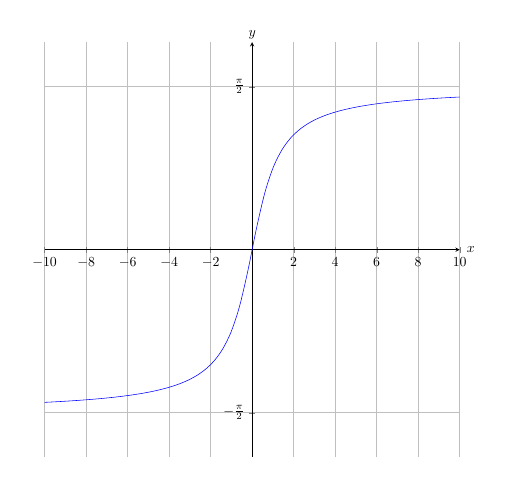
\begin{tikzpicture}[scale=.5]
		\begin{axis}[
			xmin=-10,xmax=10,
			ymin=-2,ymax=2,
			grid=both,width=\textwidth,height=\textwidth,
			axis lines=middle,
			xlabel=$x$,
			ylabel=$y$,
			enlarge x limits=0.1,
			enlarge y limits=0.1,
			axis lines = middle,
			x label style={at={(ticklabel* cs:1.00)}, inner sep=5pt, anchor=west},
			y label style={at={(ticklabel* cs:1.00)}, inner sep=2pt, anchor=south},
			ytick={-1.5708,1.5708},
			yticklabels={
				$-\frac{\pi}{2}$,
				$\frac{\pi}{2}$,
			},
		]
			\addplot[color=blue,samples=50,smooth,domain=-10:10,variable=\x]{atan(\x)/180*pi};
		\end{axis}
	\end{tikzpicture}
	\caption{反正切函数\(y=\arctan x\)的图形}
	\label{figure:函数.反正切函数的图形}
\end{figure}

\subsection{反三角函数的性质}
\begin{theorem}[余角公式]
\begin{gather}
	\arcsin x + \arccos x = \frac{\pi}{2}, \\
	\arctan x + \arccot x = \left\{ \begin{array}{cl}
		\pi/2, & x > 0, \\
		-\pi/2, & x < 0.
	\end{array} \right.
\end{gather}
\end{theorem}

\begin{theorem}[负数关系]
\begin{gather}
	\arcsin(-x) = -\arcsin x, \\
	\arccos(-x) = \pi-\arccos x, \\
	\arctan(-x) = -\arctan x, \\
	\arccot(-x) = \pi-\arccot x, \\
	\arcsec(-x) = \pi-\arcsec x, \\
	\arccsc(-x) = -\arccsc x.
\end{gather}
\end{theorem}

\begin{theorem}[倒数关系]
\begin{gather}
	\arcsin\frac{1}{x} = \arccsc x, \\
	\arccos\frac{1}{x} = \arcsec x, \\
	\arctan\frac{1}{x} = \arccot x
		= \frac{\pi}{2} - \arctan x
	\quad(x>0), \\
	\arccot\frac{1}{x} = \begin{cases}
		\arctan x, & x>0, \\
		\pi+\arctan x, & x<0,
		\end{cases} \\
	\arccot\frac{1}{x} = \left\{ \def\arraystretch{1.5} \begin{array}{lc}
		\dfrac{\pi}{2} - \arccot x, & x>0, \\
		\dfrac{3\pi}{2} - \arccot x, & x<0,
		\end{array} \right. \\
	\arcsec\frac{1}{x} = \arccos x, \\
	\arccsc\frac{1}{x} = \arcsin x.
\end{gather}
\end{theorem}

\begin{theorem}[三角关系]
\begin{gather}
	\sin(\arcsin{x}) = x, \\
	\cos(\arccos{x}) = x, \\
	\tan(\arctan{x}) = x, \\
	\arcsin(\sin x) = x, \quad x \in (-\frac{\pi}{2},\frac{\pi}{2}), \\
	\arccos(\cos x) = x, \quad x \in (0,\pi), \\
	\arctan(\tan x) = x, \quad x \in (-\frac{\pi}{2},\frac{\pi}{2}), \\
	\sin(\arccos{x}) = \cos(\arcsin{x}) = \sqrt{1 - x^2}, \\
	\tan(\arccot{x}) = \cot(\arccot{x}) = \frac{1}{x}, \\
	\sin(\arctan{x}) = \cos(\arccot{x}) = \frac{x}{\sqrt{1+x^2}}, \\
	\cos(\arctan{x}) = \sin(\arccot{x}) = \frac{1}{\sqrt{1+x^2}}.
\end{gather}
\end{theorem}

\begin{theorem}[和差公式]
\begin{align}
&\hspace{-10pt}
\arcsin x + \arcsin y \\
	&= \arcsin(x \sqrt{1-y^2} + y \sqrt{1-x^2})
		\quad(xy\leq0 \lor x^2+y^2\leq1) \\
	&= \pi - \arcsin(x \sqrt{1-y^2} + y \sqrt{1-x^2})
		\quad(x>0, y>0, x^2+y^2>1) \\
	&= -\pi - \arcsin(x \sqrt{1-y^2} + y \sqrt{1-x^2})
		\quad(x<0, y<0, x^2+y^2>1), \\
&\hspace{-10pt}
\arcsin x - \arcsin y \\
	&= \arcsin(x \sqrt{1-y^2} - y \sqrt{1-x^2})
		\quad(xy\geq0 \lor x^2+y^2\leq1) \\
	&= \pi - \arcsin(x \sqrt{1-y^2} - y \sqrt{1-x^2})
		\quad(x>0, y<0, x^2+y^2>1) \\
	&= -\pi - \arcsin(x \sqrt{1-y^2} + y \sqrt{1-x^2})
		\quad(x<0, y>0, x^2+y^2>1), \\
&\hspace{-10pt}
\arccos x + \arccos y \\
	&= \arccos[xy - \sqrt{(1-x^2)(1-y^2)}]
		\quad(x+y\geq0) \\
	&= 2\pi - \arccos[xy - \sqrt{(1-x^2)(1-y^2)}]
		\quad(x+y<0), \\
&\hspace{-10pt}
\arccos x - \arccos y \\
	&= -\arccos[xy + \sqrt{(1-x^2)(1-y^2)}]
		\quad(x \geq y) \\
	&= \arccos[xy + \sqrt{(1-x^2)(1-y^2)}]
		\quad(x<y), \\
&\hspace{-10pt}
\arctan x + \arctan y \\
	&= \arctan\frac{x+y}{1-xy}
		\quad(xy<1) \\
	&= \pi+\arctan\frac{x+y}{1-xy}
		\quad(x>0,xy>1) \\
	&= -\pi+\arctan\frac{x+y}{1-xy}
		\quad(x<0,xy>1), \\
&\hspace{-10pt}
\arctan x - \arctan y \\
	&= \arctan\frac{x-y}{1+xy}
		\quad(xy>-1) \\
	&= \pi+\arctan\frac{x-y}{1+xy}
		\quad(x>0,xy<-1) \\
	&= -\pi+\arctan\frac{x-y}{1+xy}
		\quad(x<0,xy<-1).
\end{align}
\end{theorem}

\begin{figure}[ht]
	\centering
	\begin{tikzpicture}
		\draw[help lines, color=gray!30, dashed](0,0)grid(4,3);
		\coordinate(A)at(0,0);
		\coordinate(B)at(4,0);
		\coordinate(C)at(4,3);
		\draw (A)node[left]{\(A\)}
			--(B)node[right]{\(B\)}node[midway,below]{\(1\)}
			--(C)node[right]{\(C\)}node[midway,right]{\(x\)}
			--(A)node[midway,above left]{\(\sqrt{1+x^2}\)}
			pic["\(\theta\)",draw=orange,-,angle eccentricity=2,angle radius=0.3cm]{angle=B--A--C}
			pic[draw=gray,-,angle radius=0.3cm]{right angle=C--B--A};
		\draw (5,1.5)node[right]{\(\begin{aligned}
			&\tan\theta = x \implies \theta = \arctan x, \\
			&\cos\theta = \cos(\arctan x) = \frac{1}{\sqrt{1+x^2}}, \\
			&\sin\theta = \sin(\arctan x) = \frac{x}{\sqrt{1+x^2}}, \\
			&\cot\theta = \cot(\arctan x) = \frac{1}{x}.
		\end{aligned}\)};
	\end{tikzpicture}
	\caption{三角函数与反三角函数之间的联系}
\end{figure}

\section{双曲函数、反双曲函数}
\begin{definition}[双曲函数]
\begin{gather}
	\sinh x \defeq \frac{e^x - e^{-x}}2. \\
	\cosh x \defeq \frac{e^x + e^{-x}}2. \\
	\tanh x \defeq \frac{\sinh x}{\cosh x}. \\
	\coth x \defeq \frac{\cosh x}{\sinh x}. \\
	\sech x \defeq \frac1{\cosh x}. \\
	\csch x \defeq \frac1{\sinh x}.
\end{gather}
这里,
\(\sinh x\)被称为\DefineConcept{双曲正弦},
\(\cosh x\)被称为\DefineConcept{双曲余弦},
\(\tanh x\)被称为\DefineConcept{双曲正切},
\(\coth x\)被称为\DefineConcept{双曲余切}.
\end{definition}

可以看出\begin{gather*}
	\tanh x = \frac{e^x - e^{-x}}{e^x + e^{-x}}. \\
	\coth x = \frac{e^x + e^{-x}}{e^x - e^{-x}}.
\end{gather*}

\begin{figure}[ht]
	\centering
	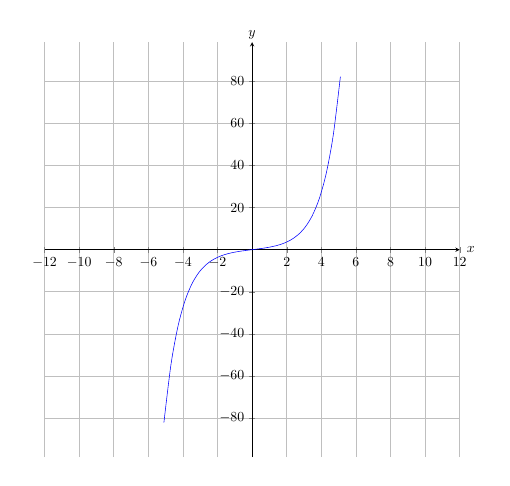
\begin{tikzpicture}[scale=.5]
		\begin{axis}[
			xmin=-10,xmax=10,
			restrict y to domain=-100:100,
			grid=both,width=\textwidth,height=\textwidth,
			axis lines=middle,
			xlabel=$x$,
			ylabel=$y$,
			enlarge x limits=0.1,
			enlarge y limits=0.1,
			x label style={at={(ticklabel* cs:1.00)}, inner sep=5pt, anchor=west},
			y label style={at={(ticklabel* cs:1.00)}, inner sep=2pt, anchor=south},
		]
			\addplot[color=blue,samples=50,smooth,domain=-10:10]{.5*(exp(x)-exp(-x))};
		\end{axis}
	\end{tikzpicture}
	\caption{双曲正弦函数的图形}
	\label{figure:函数.双曲正弦函数的图形}
\end{figure}

\begin{figure}[ht]
	\centering
	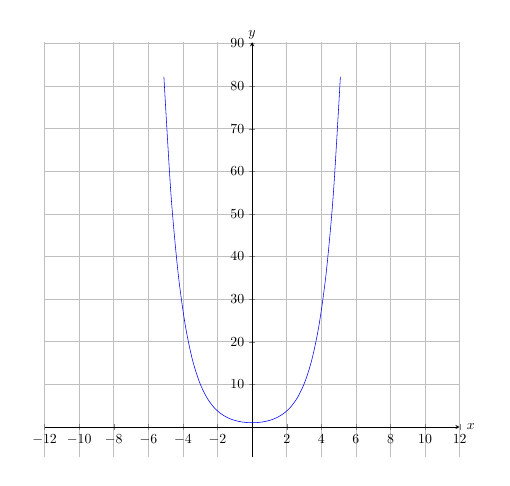
\begin{tikzpicture}[scale=.5]
		\begin{axis}[
			xmin=-10,xmax=10,
			restrict y to domain=-100:100,
			grid=both,width=\textwidth,height=\textwidth,
			axis lines=middle,
			xlabel=$x$,
			ylabel=$y$,
			enlarge x limits=0.1,
			enlarge y limits=0.1,
			x label style={at={(ticklabel* cs:1.00)}, inner sep=5pt, anchor=west},
			y label style={at={(ticklabel* cs:1.00)}, inner sep=2pt, anchor=south},
		]
			\addplot[color=blue,samples=50,smooth,domain=-10:10]{.5*(exp(x)+exp(-x))};
		\end{axis}
	\end{tikzpicture}
	\caption{双曲余弦函数的图形}
	\label{figure:函数.双曲余弦函数的图形}
\end{figure}

\begin{figure}[ht]
	\centering
	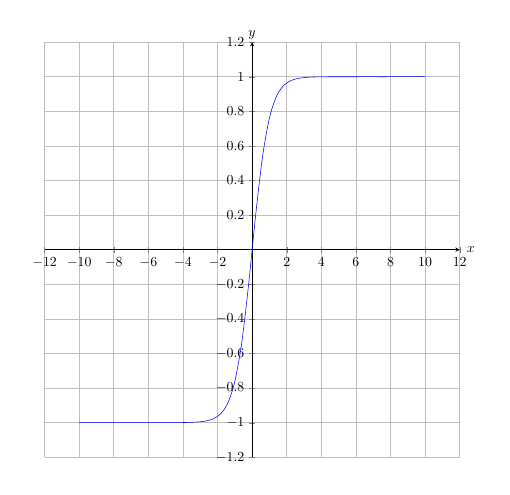
\begin{tikzpicture}[scale=.5]
		\begin{axis}[
			xmin=-10,xmax=10,
			restrict y to domain=-100:100,
			grid=both,width=\textwidth,height=\textwidth,
			axis lines=middle,
			xlabel=$x$,
			ylabel=$y$,
			enlarge x limits=0.1,
			enlarge y limits=0.1,
			x label style={at={(ticklabel* cs:1.00)}, inner sep=5pt, anchor=west},
			y label style={at={(ticklabel* cs:1.00)}, inner sep=2pt, anchor=south},
		]
			\addplot[color=blue,samples=50,smooth,domain=-10:10]{(exp(x)-exp(-x))/(exp(x)+exp(-x))};
		\end{axis}
	\end{tikzpicture}
	\caption{双曲正切函数的图形}
	\label{figure:函数.双曲正切函数的图形}
\end{figure}

\begin{figure}[ht]
	\centering
	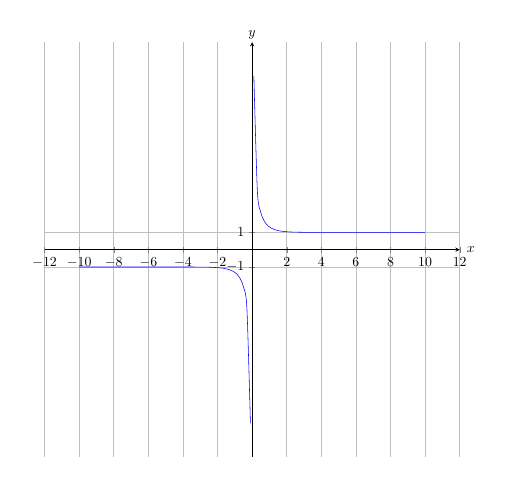
\begin{tikzpicture}[scale=.5]
		\begin{axis}[
			xmin=-10,xmax=10,
			ymin=-10,ymax=10,
			grid=both,width=\textwidth,height=\textwidth,
			axis lines=middle,
			xlabel=$x$,
			ylabel=$y$,
			enlarge x limits=0.1,
			enlarge y limits=0.1,
			x label style={at={(ticklabel* cs:1.00)}, inner sep=5pt, anchor=west},
			y label style={at={(ticklabel* cs:1.00)}, inner sep=2pt, anchor=south},
			ytick={-1,1},
		]
			\addplot[color=blue,samples=50,smooth,domain=-10:-.1]
				{(exp(x)+exp(-x))/(exp(x)-exp(-x))};
			\addplot[color=blue,samples=50,smooth,domain=.1:10]
				{(exp(x)+exp(-x))/(exp(x)-exp(-x))};
		\end{axis}
	\end{tikzpicture}
	\caption{双曲余切函数\(y=\coth x\)的图形}
	\label{figure:函数.双曲余切函数的图形}
\end{figure}

下面我们研究双曲函数的反函数.

首先讨论双曲正弦\(y=\sinh x\)的反函数.
由\(x=\sinh y\),有\[
	x=\frac{e^y-e^{-y}}{2}.
\]
令\(u=e^y\),则有\[
	u^2-2xu-1=0.
\]
这是一个关于\(u\)的一元二次方程,解得\[
	u=x\pm\sqrt{x^2+1}.
\]
因为\(u=e^y>0\),故上式根号前应取正号,即\[
	u=x+\sqrt{x^2+1}.
\]
又由\(y=\ln u\),故得反双曲正弦\[
	\arsinh x
	\defeq
	\ln(x+\sqrt{x^2+1}),
	\quad -\infty<x<+\infty.
\]

接下来讨论双曲余弦函数\(y=\cosh x\)的反函数.
由\(x=\cosh y\),有\[
	x=\frac{e^y+e^{-y}}{2},
\]
显然恒有\(x>0\).
由此得\(e^y=x\pm\sqrt{x^2-1}\ (x\geq1)\),
故\[
	y=\ln(x\pm\sqrt{x^2-1})
	\quad(x\geq1).
\]
可见,函数\[
	y=\ln(x+\sqrt{x^2-1})
	\quad(x\geq1)
\]是双曲余弦函数右支\(y=\cosh x\ (x\geq0)\)的反函数,
我们把它记作\(\arcosh x\),
即\[
	\arcosh x
	\defeq
	\ln(x + \sqrt{x^2 - 1}),
	\quad 1\leq x<+\infty.
\]
而函数\[
	y=\ln(x-\sqrt{x^2-1})
	\quad(x\geq1)
\]是双曲余弦函数左支\(y=\cosh x\ (x\leq0)\)的反函数.

易见\[
	\ln(x+\sqrt{x^2-1}) + \ln(x-\sqrt{x^2-1}) = 0
	\quad(x\geq1).
\]
%Mathematica: FullSimplify[Log[x + Sqrt[x^2 - 1]] + Log[x - Sqrt[x^2 - 1]], Assumptions -> {x >= 1}]
%@credit: {cee35532-e299-4587-89a0-7b84e7454774}

类似地可得反双曲正切\[
	\artanh x
	\defeq
	\frac{1}{2} \ln\frac{1 + x}{1 - x},
	\quad -1<x<1;
\]
以及反双曲余切\[
	\arcoth x
	\defeq
	\frac{1}{2} \ln\frac{x + 1}{x - 1},
	\quad -\infty<x<-1\lor1<x<+\infty.
\]

\begin{property}
\(\sinh x\)是奇函数,即对\(\forall x \in [-a,a]\)有\[
	\sinh(-x) = -\sinh x;
\]

\(\cosh x\)是偶函数,即对\(\forall x \in [-a,a]\)有\[
	\cosh(-x) = \cosh x.
\]
\end{property}

\begin{property}
\(\cosh x\)有下界:\[
	\cosh x \geq 1
\]
当且仅当\(x=0\)时,上式取等号.
\end{property}

\begin{theorem}
\begin{gather}
	\sinh(x \pm y) = \sinh x\cosh y \pm \cosh x\sinh y, \\
	\cosh(x \pm y) = \cosh x\cosh y \pm \sinh x\sinh y, \\
	\tanh(x + y) = \frac{\tanh x + \tanh y}{1 + \tanh x\tanh y}.
\end{gather}
\begin{proof}
根据双曲函数的定义有
\begin{align*}
	\sinh x\cosh y+\cosh x\sinh y
	&= \frac{e^x - e^{-x}}{2} \frac{e^y + e^{-y}}{2}
		+ \frac{e^x + e^{-x}}{2} \frac{e^y - e^{-y}}{2} \\
	&= \frac{1}{4} (e^x e^y + e^x e^{-y} - e^{-x} e^y - e^{-x} e^{-y} \\
	&\qquad+ e^x e^y - e^x e^{-y} + e^{-x} e^y - e^{-x} e^{-y}) \\
	&= \frac{1}{4} (2 e^x e^y - 2 e^{-x} e^{-y}) \\
	&= \frac{1}{2} (e^{x+y} - e^{-x-y}) = \sinh(x+y).
\end{align*}
\begin{align*}
	\cosh x\cosh y+\sinh x\sinh y
	&= \frac{e^x + e^{-1}}{2} \frac{e^y + e^{-y}}{2}
		+ \frac{e^x - e^{-x}}{2} \frac{e^y - e^{-y}}{2} \\
	&= \frac{1}{4} (e^x e^y + e^x e^{-y} + e^{-x} e^y + e^{-x} e^{-y} \\
	&\qquad+ e^x e^y - e^x e^{-y} - e^{-x} e^y + e^{-x} e^{-y}) \\
	&= \frac{1}{4} (2 e^x e^y + 2 e^{-x} e^{-y}) \\
	&= \frac{1}{2} (e^{x+y} + e^{-x-y}) = \cosh(x+y).
	\qedhere
\end{align*}
\end{proof}
\end{theorem}

\begin{theorem}
\begin{gather}
	\cosh^2x - \sinh^2x = 1, \\
	\sinh x + \cosh x = e^x, \\
	\cosh x - \sinh x = e^{-x}, \\
	1 - \tanh^2 x = \sech^2 x, \\
	\coth^2 x - 1 = \csch^2 x.
\end{gather}
\begin{proof}
根据双曲函数的定义有
\begin{align*}
	\cosh^2x-\sinh^2x
	&=\left(\frac{e^x + e^{-x}}{2}\right)^2-\left(\frac{e^x - e^{-x}}{2}\right)^2 \\
	&=\frac{e^{2x}+2+e^{-2x}}{4}-\frac{e^{2x}-2+e^{-2x}}{4}
	=1.
	\qedhere
\end{align*}
\end{proof}
\end{theorem}

\begin{theorem}
\begin{gather}
	\sinh2x = 2 \sinh x\cosh x, \\
	\cosh2x = \cosh^2x + \sinh^2x.
\end{gather}
\end{theorem}

\section{幂指函数}
\begin{definition}
形如\[
	y = u(x)^{v(x)},
	\quad u(x) > 0 \land u(x) \not\equiv 1
\]的函数称为\DefineConcept{幂指函数}.
\end{definition}
值得注意的是,幂指函数不是初等函数.

% \section{其他常见函数}
\subsection{单位阶跃函数}
\begin{definition}
函数\[
f(x) = \left\{ \begin{array}{cc}
0, & x < 0, \\
1, & x \geq 1
\end{array} \right.
\]称为\DefineConcept{单位阶跃函数}或\DefineConcept{赫维赛德阶跃函数}.
\end{definition}

\begin{figure}[ht]
	\centering
	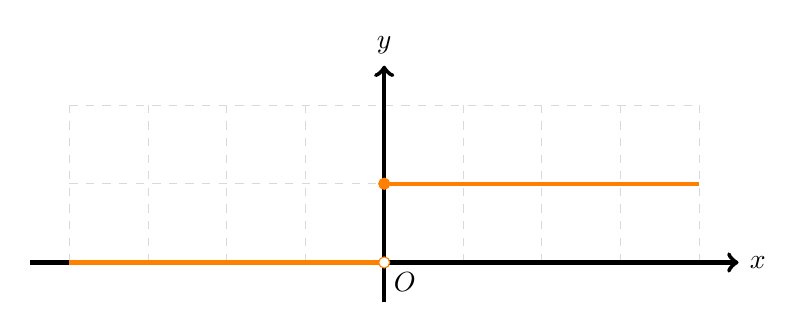
\begin{tikzpicture}
		\draw[help lines,color=gray!30,dashed](-4,0)grid(4,2);
		\draw[->,ultra thick](-4.5,0)--(4.5,0)node[right]{\(x\)};
		\draw[->,ultra thick](0,-.5)--(0,2.5)node[above]{\(y\)};
		\draw (0,0)node[below right]{\(O\)};
		\draw[orange,ultra thick](-4,0)--(0,0) (0,1)--(4,1);
		\draw[draw=orange,fill=orange](0,1)circle(2pt);
		\draw[draw=orange,fill=white](0,0)circle(2pt);
	\end{tikzpicture}
	\caption{单位阶跃函数的图形}
\end{figure}

\subsection{克罗内克\texorpdfstring{\(\delta\)}{\textdelta}函数}
\begin{definition}
%@see: https://mathworld.wolfram.com/KroneckerDelta.html
定义:\[
\delta_K(a,b)
\defeq \left\{ \begin{array}{cl}
	1, & a = b, \\
	0, & a \neq b.
\end{array} \right.
\]称其为\DefineConcept{克罗内克\(\delta\)函数}.
\end{definition}

\subsection{狄拉克\texorpdfstring{\(\delta\)}{\textdelta}函数}
\begin{definition}
%@see: https://functions.wolfram.com/GeneralizedFunctions/DiracDelta/02/
%@see: https://functions.wolfram.com/GeneralizedFunctions/DiracDelta2/02/
定义:\[
	\delta_D(x)
	\defeq \frac{1}{\pi}
		\lim\limits_{\epsilon\to0}
		\frac{\epsilon}{x^2+\epsilon^2}
	\quad(x\in\mathbb{R}).
\]
称其为\DefineConcept{狄拉克\(\delta\)函数}.
\end{definition}

\section{抽象函数}
方程\[
f(x+y) = f(x) + f(y) + c
\]确定的函数\(f\)称为直线型抽象函数,
其中\(c\)是与\(x\)、\(y\)无关的常数.

方程\[
f(xy) = f(x) f(y)
\]确定的函数\(f\)称为幂函数型抽象函数.

方程\[
f(x+y) = f(x) f(y)
\]或\[
f(xy) = [f(x)]^y
\]确定的函数\(f\)称为指数函数型抽象函数.

方程\[
f(xy) = f(x) + f(y)
\]或\[
f\left(\frac{x}{y}\right) = f(x) - f(y)
\]确定的函数\(f\)称为对数函数型抽象函数.

方程\[
f(x) + f(y) = 2 f\left(\frac{x+y}{2}\right) f\left(\frac{x-y}{2}\right)
\]或\[
f(x+y) = \frac{f(x) + f(y)}{1 - f(x) f(y)}
\]确定的函数\(f\)称为三角函数型抽象函数.

\section{初等函数}
\begin{definition}
\emph{常函数}、\emph{幂函数}、\emph{指数函数}、\emph{对数函数}、\emph{三角函数}、\emph{反三角函数}这六类函数统称为\DefineConcept{基本初等函数}.
由常数和基本初等函数经过有限次四则运算和有限次函数复合步骤所构成并可用一个式子表示的函数,称为\DefineConcept{初等函数}.
\end{definition}



\chapter{数列}
\section{数列的概念}
\begin{definition}\label{definition.数列.数列的定义}
一般地,如果\(D \subseteq \mathbb{Z}\),%
那么称映射\[
    f\colon D\to\mathbb{R}, n \mapsto a_n
\]为一个\DefineConcept{数列}(sequence,progression),
记作\(\{a_n\}\),即\(\{a_n\} \defeq f\).

数列中的每一个数(例如\(\AutoTuple{a}{0}\))叫做数列的\DefineConcept{项}(term).
表示第\(n\)个数的公式叫做数列的\DefineConcept{一般项}.
\end{definition}

应该指出,如果我们说“数列\(\{x_n\}\)在数集\(X\)内”或\(\{x_n\} \subseteq X\),
我们指的是:把数列\(\{x_n\}\)看作一个映射\(f\)时,
这个映射的值域是\(X\)的子集,即\(\ran f \subseteq X\).

\begin{definition}
如果数列\(\{x_n\}\)满足条件\[
x_n \leqslant x_{n+1}, \quad n=1,2,\dotsc,
\]就称“数列\(\{x_n\}\)是\DefineConcept{单调增加的}”;
如果数列\(\{x_n\}\)满足条件\[
x_n \geqslant x_{n+1}, \quad n=1,2,\dotsc,
\]就称“数列\(\{x_n\}\)是\DefineConcept{单调减少的}”.

单调增加数列和单调减少数列统称为\DefineConcept{单调数列}.
\end{definition}

\section{数列的连加与连乘}
\subsection{数列的连加}
\begin{definition}[连加]
定义\DefineConcept{连续求和}:\[
\sum\limits_{i=m}^n a_i
\defeq
a_m + a_{m+1} + \dotsb + a_{n-1} + a_n
\quad(m \leqslant n),
\]其中符号\(\sum\)称作\DefineConcept{连加号},%
整数\(i\)称为\DefineConcept{求和指标}(index of summation).
\end{definition}

有时候也把\(\sum\limits_{i=m}^n\)%
写作\(\sum\limits_{m \leqslant i \leqslant n}\).

使用双重连加号求和时,如果两个求和指标独立取值,则连加号\(\sum\)的顺序可以交换.

在不引起误解的情况下,可以省略不写求和指标,
例如用\(\sum a_n\)表示\(\sum\limits_{k=1}^n a_k\).

\subsection{数列的连乘}
\begin{definition}[连乘]
定义\DefineConcept{连续求积}:\[
\prod\limits_{i=m}^n a_i
\defeq
a_m \times a_{m+1} \times \dotsb \times a_{n-1} \times a_n
\quad(m \leqslant n),
\]其中符号\(\prod\)称作\DefineConcept{连乘号},整数\(i\)称为\DefineConcept{求积指标}.
\end{definition}

同样地,有时候也把\(\prod\limits_{i=m}^n\)%
写作\(\prod\limits_{m \leqslant i \leqslant n}\).

\begin{definition}\label{definition:数列.阶乘的定义}
给定一个正整数\(n\),%
称所有小于或等于\(n\)的正整数的积为“\(n\)的\DefineConcept{阶乘}(factorial)”,%
记作\(n!\),即
\begin{equation}
n!
\defeq
\prod\limits_{k=1}^n k
=
n \times (n-1) \times (n-2) \times \dotsm \times 2 \times 1.
\end{equation}
特别地,规定\(0! = 1\).
\end{definition}

\begin{definition}
给定一个正整数\(n\),%
称小于或等于\(n\)且与之同奇偶的所有正整数的积为“\(n\)的\DefineConcept{双阶乘}”,%
记作\(n!!\),即
\begin{equation}
n!!
\defeq
\begin{cases}
n \times (n-2) \times (n-4) \times \dotsm \times 3 \times 1, & n\text{是奇数}, \\
n \times (n-2) \times (n-4) \times \dotsm \times 4 \times 2, & n\text{是偶数}.
\end{cases}
\end{equation}
特别地,规定\(0!! = 1\).
\end{definition}

需要注意的是,通常来说双阶乘\(n!!\)并不等于“阶乘的阶乘”\((n!)!\),%
实际上,\(3!! = 3\)而\((3!)! = 6! = 720\).

称\(\sum\limits_{k=1}^n a_k\)为数列\(\{a_n\}\)的\DefineConcept{前\(n\)项和}.

\section{等差数列}
一般地,如果一个数列从第2项起,每一项与它的前一项的差等于同一个常数,
这个数列就叫做\DefineConcept{等差数列}(arithmetical progression),
这个常数叫做等差数列的\DefineConcept{公差}(common difference).

如果数列\(\{a_n\}\)是等差数列,它的公差是\(d\),那么\begin{align*}
    a_2 &= a_1 + d, \\
    a_3 &= a_2 + d = (a_1 + d) + d = a_1 + 2d, \\
    a_4 &= a_3 + d = (a_1 + 2d) + d = a_1 + d3.
\end{align*}
以此类推,可知等差数列\(\{a_n\}\)的\DefineConcept{通项公式}是\begin{equation}
    a_n = a_1 + (n-1) d.
\end{equation}

将等差数列中任意两项\[
    a_m = a_1 + (m-1) d
    \quad\text{与}\quad
    a_n = a_1 + (n-1) d
\]相减,得到\[
    a_m - a_n = (m-n) d.
\]
由此我们也可得到%
等差数列的\DefineConcept{递推公式}:\begin{equation}
    a_{n+1} - a_n = d.
\end{equation}

\begin{property}[等差数列求和]
设数列\(\{a_n\}\)为等差数列,它的通项公式为\[
    a_n = a_1 + (n-1) d,
\]
那么它的前\(n\)项和为\begin{equation}\label{equation:数列.等差数列的前n项和1}
    S_n = \frac{n(a_1 + a_n)}{2},
\end{equation}
或\begin{equation}\label{equation:数列.等差数列的前n项和2}
    S_n = n a_1 + \frac{n(n-1)}{2} d.
\end{equation}
\begin{proof}
由\[
    S_n = a_1 + (a_1 + d) + \dotsb + [a_1 + (n-2)d] + [a_1 + (n-1)d],
\]\[
    S_n = [a_n - (n-1)d] + [a_n - (n-2)d] + \dotsb + (a_n - d) + a_n,
\]相加得\[
    2 S_n = n(a_1 + a_n),
\]最终可得\[
    S_n = \frac{n(a_1 + a_n)}{2} = n a_1 + \frac{n(n-1)}{2} d.
    \qedhere
\]
\end{proof}
\end{property}

根据\hyperref[equation:数列.等差数列的前n项和1]{等差数列的前\(n\)项和公式},立即有如下结论:
\begin{equation}
    \sum\limits_{k=1}^n k = \frac{1}{2} n(n+1).
\end{equation}

\section{平方数列}
如果数列\(\{a_n\}\)的通项公式是\[
a_n = n^2,
\]那么称其为\DefineConcept{平方数列}.

由立方差公式可知
\[\begin{aligned}
n^3 - (n-1)^3
&= [n - (n-1)] \cdot [n^2 + n(n-1) + (n-1)^2] \\
&= 2n^2 + (n-1)^2 - n.
\end{aligned}\]于是将\[
\begin{array}{l}
2^3 - 1^3 = 2\times2^2+1^2-2, \\
3^3 - 2^3 = 2\times3^2+2^2-3, \\
\hdotsfor{1} \\
n^3 - (n-1)^3 = 2n^2 + (n-1)^2 - n,
\end{array}
\]相加便得\[\begin{aligned}
n^3 - 1^3
&= 2(2^2+3^2+\dotsb+n^2) + [1^2+2^2+\dotsb+(n-1)^2] - (2+3+\dotsb+n) \\
&= 2\left(\sum\limits_{k=1}^n k^2 - 1\right)
    + \left(\sum\limits_{k=1}^n k^2 - n^2\right)
    - \left(\sum\limits_{k=1}^n k - 1\right) \\
&= 3\sum\limits_{k=1}^n k^2 - 2 - n^2 - \frac{n(n+1)}{2} + 1 \\
&= 3\sum\limits_{k=1}^n k^2 - \frac{3}{2} n^2 - \frac{1}{2} n - 1,
\end{aligned}\]
移项,得\[
3 \sum\limits_{k=1}^n k^2
= n^3 + \frac{3}{2} n^2 + \frac{1}{2} n
= \frac{1}{2} n (n+1) (2n+1).
\]
因此,平方数列的前\(n\)项之和为
\begin{equation}
\sum\limits_{k=1}^n a_n
= \sum\limits_{k=1}^n k^2
= \frac{1}{6} n(n+1)(2n+1).
\end{equation}

\begin{example}
求在正方形底上排成完整棱锥体的小球个数.
\begin{solution}
设底部每边有\(n\)个小球,则最底层小球的个数为\(n^2\)个;
从下往上数,第二层有\((n-1)^2\)个小球,
第三层有\((n-2)^2\)个小球,
以此类推,直至顶层只有一个小球.
因此,棱锥体的小球个数为\[
    S = n^2+(n-1)^2+(n-2)^2+\dotsb+1
    = \frac{n(n+1)(2n+1)}{6}.
\]
\end{solution}
\end{example}

\begin{example}
求在等边三角形底上排成完整棱锥体的小球个数.
\begin{solution}
设底部每边有\(n\)个小球,则最底层小球的个数为\[
    n+(n-1)+(n-2)+\dotsb+1
    = \frac{n(n+1)}{2}
    = \frac{1}{2}(n^2+n).
\]
在上式中以\((n-1),(n-2),\dotsc\)替代\(n\),
就得到了从下往上数从第二层开始直至最顶层的小球个数.
因此,棱锥体的小球个数为\[
    S = \frac{1}{2} (\sum n^2 + \sum n)
    = \frac{n(n+1)(n+2)}{6}.
\]
\end{solution}
\end{example}

\section{立方数列}
如果数列\(\{a_n\}\)的通项公式是\[
a_n = n^3,
\]那么称其为\DefineConcept{立方数列}.

由平方差公式可知
\[\begin{aligned}
n^4 - (n-1)^4
&= [n^2 - (n-1)^2] [n^2 + (n-1)^2] \\
&= [n - (n-1)] [n + (n-1)] [n^2 + (n-1)^2] \\
&= (2n-1) (2n^2 - 2n + 1) \\
&= 4n^3 - 6n^2 + 4n - 1.
\end{aligned}\]
于是\[
\sum\limits_{k=1}^n [k^4 - (k-1)^4]
= \sum\limits_{k=1}^n (4k^3 - 6k^2 + 4k - 1),
\]即\[\begin{aligned}
n^4
&= 4 \sum\limits_{k=1}^n k^3 - 6 \sum\limits_{k=1}^n k^2 + 4 \sum\limits_{k=1}^n k - n \\
&= 4 \sum\limits_{k=1}^n k^3 - n(n+1)(2n+1) + 2n(n+1) - n,
\end{aligned}\]
移项,得\[
4 \sum\limits_{k=1}^n k^3
= n^4 + n(n+1)(2n+1) - 2n(n+1) + n
= n^4 + 2n^3 + n^2
= n^2(n+1)^2.
\]
因此,立方数列的前\(n\)项之和为
\begin{equation}
\sum\limits_{k=1}^n a_n
= \sum\limits_{k=1}^n k^3
= \left[\frac{n(n+1)}{2}\right]^2.
\end{equation}

\section{等比数列}
\begin{definition}
如果数列\(\{a_n\}\)满足\[
a_n = a_1 q^{n-1} \quad(q\neq1),
\]则称该数列为\DefineConcept{等比数列}或\DefineConcept{几何数列}(geometrical progression),
其中\(q\)称作\DefineConcept{公比}.

等比数列的递推公式为\(\frac{a_n}{a_{n-1}} = q\)(\(n \geqslant 2\)).
\end{definition}

\begin{property}[等比数列求和]
设数列\(\{a_n\}\)为等比数列\[
a_n = a_1 q^{n-1} \qquad (q \neq 1)
\]则有\[
S_n = \sum\limits_{i=1}^n a_i
= \left\{ \begin{array}{cl}
\frac{a_1 (q^n-1)}{q-1}, & q \neq 1, \\
na, & q = 1.
\end{array} \right.
\]
\begin{proof}
当\(q = 1\)时,显然有\(S_n = na\).
当\(q \neq 1\)时,有\[
q S_n = aq+aq^2+aq^3+\dotsb+aq^n,
\]\[
S_{n+1} = a+aq+aq^2+\dotsb+aq^{n-1}+aq^n,
\]因此\[
S_{n+1} - q S_n = a.
\]又因为\(S_{n+1} - S_n = aq^n\),所以\[
(q-1) S_n = (S_{n+1} - S_n) - (S_{n+1} - q S_n) = aq^n - a = a(q^n - 1),
\]\[
S_n = \frac{a(q^n - 1)}{q-1}.
\qedhere
\]
\end{proof}
\end{property}

\begin{property}
设数列\(\{a_n\}\)为等差数列,\(b\)为常数,则:
\begin{enumerate}
    \item \(\{b + a_n\}\)为等差数列,它的公差与\(\{a_n\}\)的一样;
    \item \(\{b \cdot a_n\}\)为等差数列,它的公差是\(\{a_n\}\)的\(b\)倍;
    \item \(\{b^{a_n}\}\)为等比数列.
\end{enumerate}
\end{property}

\begin{property}
设数列\(\{a_n\}\)为等比数列,\(b\)为常数,则:
\begin{enumerate}
    \item \(\{b \cdot a_n\}\)为等比数列,它的公比与\(\{a_n\}\)的一样;
    \item \(\{b / a_n\}\)为等比数列,它的公比是\(\{a_n\}\)的公比的倒数;
    \item \(\{\log_b a_n\}\)为等差数列.
\end{enumerate}
\end{property}

\begin{example}
求级数\[
    a,(a+d)r,(a+2d)r^2,(a+3d)r^3,\dotsc
\]的前\(n\)项之和.
\begin{solution}
设所求级数的前\(n\)项之和为\[
    S_n = \sum\limits_{k=0}^{n-1} (a+kd) r^k.
    \eqno(1)
\]
那么\[
    r S_n = \sum\limits_{k=0}^{n-1} (a+kd) r^{k+1}.
    \eqno(2)
\]
将(1)式与(2)式相减,得\begin{align*}
    S_n(1-r) &= a + (dr + dr^2 + \dotsb + dr^{n-1}) - [a+(n-1)d] r^n \\
    &= a + \frac{dr(1-r^{n-1})}{1-r} - [a+(n-1)d] r^n.
\end{align*}
于是\[
    S_n = \frac{a}{1-r} + \frac{dr(1-r^{n-1})}{(1-r)^2} - \frac{[a+(n-1)d] r^n}{1-r}.
\]
\end{solution}
\end{example}

\section{调和数列}
若数列\(\{a_n\}\)每相邻三项满足\[
    \frac{a_{n+1}}{a_{n-1}}
    = \frac{a_{n+1}-a_n}{a_n-a_{n-1}},
\]
则称其为\DefineConcept{调和数列}(harmonical progression)\footnote{%
人们对调和数列有兴趣的主要原因是它在几何学与声学中有其重要性.
调和数列的若干项求和无一般公式可循.
通常来说,涉及调和数列的问题的解法都是将它的各项倒转,再利用对应的等差数列的性质.
};
称\(a_n\)为“\(a_{n-1}\)和\(a_{n+1}\)的\DefineConcept{调和中项}或\DefineConcept{调和平均数}”.

\begin{property}\label{theorem:数列.调和数列的性质}
调和数列\(\{a_n\}\)各项的倒数组成的数列\(\{1/a_n\}\)是等差数列.
\begin{proof}
根据调和数列的定义可知,\[
    \frac{a_{n+1}}{a_{n-1}}
    = \frac{a_{n+1}-a_n}{a_n-a_{n-1}},
\]整理得\[
    a_{n+1} (a_n - a_{n-1})
    = a_{n-1} (a_{n+1} - a_n),
\]再同除以\((a_{n+1} \cdot a_n \cdot a_{n-1})\),得\[
    \frac{1}{a_{n-1}} - \frac{1}{a_n}
    = \frac{1}{a_n} - \frac{1}{a_{n+1}}.
    \qedhere
\]
\end{proof}
\end{property}

\begin{example}
求\(a\)与\(b\)的调和平均数.
\begin{solution}
设\(a\)与\(b\)的调和平均数为\(h\).
由\cref{theorem:数列.调和数列的性质} 有\[
    \frac{1}{h} - \frac{1}{a}
    = \frac{1}{b} - \frac{1}{h},
\]\[
    \frac{2}{h} = \frac{1}{a} + \frac{1}{b}
    = \frac{a+b}{ab},
\]\[
    h = \frac{2ab}{a+b}.
\]
\end{solution}
\end{example}

我们知道,两个数\(x\)与\(y\)的算术平均数、几何平均数、调和平均数分别为\[
    A = \frac{x+y}{2}, \qquad
    G = \sqrt{xy}, \qquad
    H = \frac{2xy}{x+y}.
\]
由于\[
    A \cdot H = \frac{x+y}{2} \cdot \frac{2xy}{x+y}
    = ab = G^2,
\]
所以\(G\)又是\(A\)与\(H\)的几何平均数.
我们还注意到,当\(x,y>0\)且\(x \neq y\)时,\[
    A - G = \frac{x+y}{2} - \sqrt{xy}
    = \frac{x+y-2\sqrt{xy}}{2}
    = \left(\frac{\sqrt{x}-\sqrt{y}}{\sqrt{2}}\right)^2
    > 0,
\]
因此我们可以说:
两个正数的算术平均数总大于它们的几何平均数,即\(A > G\).
再考虑到\(G^2 = A H\),\(G\)是介于\(A\)与\(H\)之间的,于是必有\(G > H\).
综上所述,两个正数的算术平均数、几何平均数、调和平均数的大小依次递减,即\(A > G > H\).

\section{斐波那契数列}
如果数列\(\{a_n\}\)满足\(a_1=a_2=1\),且\[
a_n = a_{n-1} + a_{n-2} \quad(n\geqslant3),
\]则称该数列为\DefineConcept{斐波那契数列}.

\section{已知递推公式求解通项公式的方法}
\subsection{\texorpdfstring{形如\(a_{n+2}=p a_{n+1} + q a_n\ (q\neq0)\)的递推公式}{第一类递推公式}}
对于形如\(a_{n+2}=p a_{n+1} + q a_n\ (q\neq0)\)的递推公式,我们可以令\[
\mat{X}_n = \begin{bmatrix}
a_{n+1} \\
a_n
\end{bmatrix},
\qquad
\mat{A} = \begin{bmatrix}
p & q \\
1 & 0
\end{bmatrix},
\]则\(\mat{X}_{n+1} = \mat{A} \mat{X}_n\),从而\(\mat{X}_n = \mat{A}^{n-1} \mat{X}_1\).
这样就可以求出通项公式.

现在我们来求\(\mat{A}\)的幂.
此时\(\mat{A}\)的特征多项式为\[
f(x) = \begin{vmatrix}
x-p & -q \\
-1 & x
\end{vmatrix} = x^2 - px - q,
\]我们也称这个多项式为递推公式的特征方程.

假设我们求得该方程的两个复根为\(\alpha,\beta\),则由韦达定理可知\(p=\alpha+\beta, q=-\alpha\beta\).
注意到\[
\left\{ \begin{array}{l}
a_{n+2} - \alpha a_{n+1} = \beta(a_{n+1}-\alpha a_n), \\
a_{n+2} - \beta a_{n+1} = \alpha(a_{n+1}-\beta a_n)
\end{array} \right.,
\]从而\[
\left\{ \begin{array}{l}
a_{n+1} - \alpha a_n = \beta^{n-1} (a_2 - \alpha a_1), \\
a_{n+1} - \beta a_n = \alpha^{n-1} (a_2 - \beta a_1)
\end{array} \right.,
\]

若\(\alpha\neq\beta\),解关于\(a_{n+1},a_n\)的线性方程组可得\[
a_n = \frac{\beta^{n-1} (a_2 - \alpha a_1) - a^{n-1} (a_2 - \beta a_1)}{\beta-\alpha};
\]
若\(\alpha=\beta\),则\(\alpha=\beta\neq0\),从而\(a_{n+1} = \alpha a_n = \alpha^{n-1} (a_2 - \alpha a_1)\),进而\[
\frac{a_{n+1}}{\alpha^{n+1}} - \frac{a_n}{\alpha^n} = \frac{1}{\alpha^2}(a_2-\alpha a_1),
\]最后得到\[
a_n = (2-n)\alpha^{n-1} a_1 + (n-1) \alpha^{n-2} a_2.
\]

利用上述结论可以求出斐波那契数列的通项公式为\[
a_n = \frac{1}{\sqrt{5}} \left[
\left(\frac{1+\sqrt{5}}{2}\right)^n
-\left(\frac{1-\sqrt{5}}{2}\right)^n
\right].
\]

\subsection{\texorpdfstring{形如\(a_{n+1} = \frac{a a_n + b}{c a_n + d}\ (ad-bc\neq0)\)的递推公式}{第二类递推公式}}
对于形如\(a_{n+1} = \frac{a a_n + b}{c a_n + d}\ (ad-bc\neq0)\)的递推公式\footnote{这里\(ad-bc\neq0\)确保分式不可能恒为常数(即分式不能约分).},首先考虑特征方程\[
x = \frac{ax+b}{cx+d},
\]整理得\[
cx^2+(d-a)x-b=0,
\]解得\[
\alpha=\frac{(a-d)-\sqrt{(d-a)^2+4bc}}{2c}, \qquad
\beta=\frac{(a-d)+\sqrt{(d-a)^2+4bc}}{2c}.
\]由韦达定理,有\[
\alpha+\beta=\frac{a-d}{c}, \qquad
\alpha\beta=-\frac{b}{c};
\]因此\[
a_{n+1} = \frac{\left(\alpha+\beta+\frac{d}{c}\right) a_n - \alpha\beta}{a_n + \frac{d}{c}}.
\]

接下来分成两种情况讨论:\begin{enumerate}
\item 若\(\alpha\neq\beta\),则\[
\frac{a_{n+1}-\alpha}{a_{n+1}-\beta}
= \frac{\left(\alpha+\beta+\frac{d}{c}\right) a_n - \alpha\beta - \alpha \left(a_n + \frac{d}{c}\right)}{\left(\alpha+\beta+\frac{d}{c}\right) a_n - \alpha\beta - \beta \left(a_n + \frac{d}{c}\right)}
= \frac{c\beta+d}{c\alpha+d} \frac{a_n-\alpha}{a_n-\beta}.
\]记\(b_n = \frac{a_n-\alpha}{a_n-\beta}\),则\(b_{n+1} = \frac{c\beta+d}{c\alpha+d} b_n\).

\item 若\(\alpha=\beta=\frac{a-d}{2c}\),则\[
a_{n+1} = \frac{\left(2\alpha+\frac{d}{c}\right) a_n - \alpha^2}{a_n + \frac{d}{c}}
= \frac{(2c\alpha+d)a_n-c\alpha^2}{c a_n+d},
\]进而有\[
\frac{1}{a_{n+1}-\alpha}=\frac{1}{a_n-\alpha}+\frac{1}{\alpha+\frac{d}{c}}.
\]记\(b_n = \frac{1}{a_n-\alpha}\),则\(b_{n+1} = b_n + \frac{1}{\alpha+\frac{d}{c}}\).
\end{enumerate}
%数列
\chapter{初等代数}
\section{排列组合}
\subsection{排列、组合的基本概念}
从若干个元素中取出几个或全部的一种排法,
称作是一个\DefineConcept{排列}(permutation).
例如,从\(a,b,c,d\)四个字母里一次取出两个的排列数有12个,即\[
	\begin{gathered}
	ab, \quad
	ac, \quad
	ad, \quad
	bc, \quad
	bd, \quad
	cd, \\
	ba, \quad
	ca, \quad
	da, \quad
	cb, \quad
	db, \quad
	dc;
	\end{gathered}
\]
其中每一个都代表两个字母的不同的排法.

从若干个元素中取出几个或全部的一种选法,
称作是一个\DefineConcept{组合}(combination).
例如,从\(a,b,c,d\)四个字母里一次取出两个的组合数有6个,即\[
	ab, \quad
	ac, \quad
	ad, \quad
	bc, \quad
	bd, \quad
	cd;
\]
其中每一个都代表两个字母的不同的选法.

从这些例子中我们看到,组合仅与每个选法所含元素的个数有关,
而排列还要考虑元素在每一个排法中的次序.
例如,从四个字母\(a,b,c,d\)中选三个字母可以得到\(abc\)这样一种组合,
可以作以下六种不同的排列:\[
	abc, \quad
	acd, \quad
	bca, \quad
	bac, \quad
	cab, \quad
	cba.
\]

\subsection{排列组合的基本原理}
在讨论排列与组合的一般性命题之前,我们先通过几个例子来说明两个重要的原则.
\begin{enumerate}
	\item {\bf 加法原理}:
	如果做一件事,完成它可以有\(n\)类办法,
	在第一类办法中有\(m_1\)种不同的方法,
	在第二类办法中有\(m_2\)种不同的方法,……,
	在第\(n\)类办法中有\(m_n\)种不同的方法,那么完成这件事共有\[
	N = m_1 + m_2 + \dotsb + m_n
	\]种不同的方法.

	\item {\bf 乘法原理}:
	如果做一件事,完成它需要分成\(n\)个步骤,
	做第一步有\(m_1\)种不同的方法,
	做第二步有\(m_2\)种不同的方法,……,
	做第\(n\)步有\(m_n\)种不同的方法,那么完成这件事共有\[
	N = m_1 \times m_2 \times \dotsm \times m_n
	\]种不同的方法.
\end{enumerate}

\begin{example}
有10艘汽艇往返于利物浦与都柏林之间,问某人来回乘坐不同汽艇的方式有多少种?
\begin{solution}
去时有10种方式;对于其中每一种,因为不能乘坐同一条船,回来时有9种方式可选;
因此,一共有\(10 \times 9 = 90\)种方法来完成这两段路程.
\end{solution}
\end{example}

\begin{example}
3个旅行者来到一个小镇,镇上有4家旅店,若他们分别住不同的旅店,问投宿的方式有多少种?
\begin{solution}
第一个人可以有4种选择;
在他选定后,第二个人有3种选择;
从而这两个人共有\(4 \times 3\)种选择,
对于其中每一种选择,第三个人有2家旅店供选择;
所以,投宿的方式共有\(4 \times 3 \times 2 = 24\)种.
\end{solution}
\end{example}

我们现在来求从\(n\)个不同元素中一次取出\(k\)个的排列数.
这可以看成是用我们手上的\(n\)个不同元素去填满\(k\)个空位的不同方式的种数.

填第一个位置有\(n\)种方式,
因为可以取\(n\)个元素中的任意一个.
在这个位置用任意一种方式填好后,
填第二个位置有\(n-1\)种方式.
由于填第一个位置的每一种方式,都可与填第二个位置的每一种方式组合,
所以填前两个位置的方式有\(n(n-1)\)种.
前两个位置以任意一种方式填好后,
填第三个位置有\(n-2\)种方式.
同理,填前三个位置的方式共有\(n(n-1)(n-2)\)种.
继续这样的方法,我们注意到每填一个新的位置,就产生一个新的因子.
而且在每一步上,因子的个数总与剩余位置的个数相同;
于是,我们得出填满\(k\)个位置的方式种数等于\[
	\underbrace{n(n-1)(n-2)\dotsm[n-(k-1)]}_{k\ \text{个因子}}.
\]
这就是所求从\(n\)个元素一次取出\(k\)个元素的排列数,
我们可以利用阶乘记号将它表示为\[
	\frac{n!}{(n-k)!}.
\]

我们还可以推断出如下结论:
从\(n\)个元素一次取出全部\(n\)个元素的排列数为\(n!\).

以后我们用符号\(A_n^k\)表示从\(n\)个元素一次取出\(k\)个的排列数,即\begin{equation}
	A_n^k \defeq \frac{n!}{(n-k)!}.
\end{equation}
特别地,\(A_n^n \equiv n!\).

从\(n\)个元素一次取出\(k\)个元素的排列数也可用下面的思路求得.
按规定,我们用\(A_n^k\)代表从\(n\)个元素一次取出\(k\)个元素的排列数.
假设我们首先组成\(n\)个元素一次取出\(k-1\)个元素的所有排列,
那么这些排列一共有\(A_n^{k-1}\)种.
在这些排列的每一个的后面,我们放上剩下的\(n-(k-1)\)个元素中的任意一个;
每进行一次这样的操作,我们便得到\(n\)个元素一次取\(k\)个的一种排列,
因此,\(n\)个元素一次取\(k\)个的排列数为\(A_n^{k-1} \times (n-k+1)\)种,即\[
	A_n^k = A_n^{k-1} \times (n-k+1).
\]
在上式中用\(k-1\)代替\(k\),我们得\[
	A_n^{k-1} = A_n^{k-2} \times (n-k+2);
\]
依次递推,直到\[
	A_n^2 = A_n^1 \times (n-1),
\]\[
	A_n^1 = n.
\]
将上述各式的等号左右两边分别相乘,且约去两边相同的因子,便得\[
	A_n^k = n(n-1)\dotsm(n-k+2)(n-k+1).
\]

接下来我们想求从\(n\)个不同的元素中一次取出\(k\)的组合数.
我们用符号\(C_n^k\)表示所求组合数.
每一个这样的组合都由一组\(k\)个不同的元素组成,
而这组元素本身又可以组成\(k!\)个不同的排列.
因此\(C_n^k \times k!\)便等于\(n\)个元素一次取\(k\)个的排列数,即\[
	C_n^k \times k! \equiv A_n^k
	= n(n-1)(n-2)\dotsm(n-k+2)(n-k+1);
\]于是\begin{align}
	C_n^k &= \frac{n(n-1)(n-2)\dotsm(n-k+2)(n-k+1)}{k!} \\
	&= \frac{n!}{k! (n-k)!}.
\end{align}

需要注意到,当\(k=n\)时,有\[
	A_n^n = \frac{n!}{(n-n)!} = \frac{n!}{0!} = n!,
\]\[
	C_n^n = \frac{n!}{n! (n-n)!} = \frac{n!}{n! 0!} = \frac{1}{0!} = 1;
\]
这说明,符号\(0!\)的取值应该等于\(1\).
这就是为什么我们在\hyperref[definition:数列.阶乘的定义]{阶乘的定义}中特别规定\(0!\equiv1\).
%特别地,规定:当\(n < k\)时,\(C_n^k = 0\).

\begin{example}
将\(m+n\)颗小球分为两袋,一袋含\(m\)颗小球,另一袋含\(n\)颗小球,求可能的分法种数.
\begin{solution}
不难看出,这样的分法种数,等于从\(m+n\)颗小球中一次取\(m\)颗的组合数,
如此,可将取出的\(m\)颗小球装入一袋,将剩下的\((m+n)-m=n\)颗小球装入另一袋.
因此,所求的分法种数为\[
	\frac{(m+n)!}{m! n!}.
\]

特别地,当\(m=n\)时,两个袋子中所含小球颗数相同.
如果认为“两个袋子没有次序”或者说“袋子互换,分法种数不变”,那么分法种数为\[
	\frac{(2n)!}{(n!)^2 2!}.
\]
\end{solution}
\end{example}

\begin{example}
将\(m+n+p\)颗小球分为三袋,且各袋分别含\(m,n,p\)颗小球,求可能的分法种数.
\begin{solution}
首先将全部小球分到两个口袋里,各袋分别含\(m,n+p\)颗小球,分法种数为\[
	\frac{(m+n+p)!}{m!(n+p)!};
\]
然后将第二袋中的\(n+p\)颗小球再分为两袋,各袋分别含\(n,p\)颗小球,分法种数为\[
	\frac{(n+p)!}{n! p!};
\]
所以,全部\(m+n+p\)颗小球分成三袋,各袋分别含\(m,n,p\)颗小球的分法种数为\[
	\frac{(m+n+p)!}{m!(n+p)!} \cdot \frac{(n+p)!}{n! p!}
	= \frac{(m+n+p)!}{m! n! p!}.
\]

特别地,当\(m=n=p\)时,三个袋子中所含小球颗数相同.
如果认为“三个袋子有次序”或者说“袋子互换,就得到新的分法”,那么分法种类为\[
	\frac{(3n)!}{(n!)^3};
\]
反之,如果认为“三个袋子没有次序”,那么分法种类为\[
	\frac{(3n)!}{(n!)^3 3!}.
\]
\end{solution}
\end{example}

到目前为止,我们考虑的元素(如小球)常常被看作是不同的;
但有的时候,所给元素中有一部分元素是相同的.
相同的元素是无法区分的,不管怎么排布这些元素,都对排法种数没有影响.

\begin{example}
排列\(n\)颗小球,其中\(p\)颗是红球,\(q\)颗是黄球,\(r\)颗是蓝球,
剩余的\(n-p-q-r\)颗小球具有互不相同的彩色花纹,求可能的排列数.
\begin{solution}
当提到一组小球具有某种特征(如小球是红色的)时,
我们认为这组小球是相同的、无法区分的.
基于这条约定,我们来求解可能的排列数.

设所求排列数为\(x\).
如果用\(p\)颗花纹各异的小球代替上述\(p\)颗红球,
那么对于\(x\)个排列中的任一个,
不改变其他小球的位置,我们可以作\(p!\)个新排列;
于是如果对\(x\)个排列中的每一个,都作这样的替换,
我们就得到\(x \cdot p!\)种排列.
同理,如果在此基础上继续用\(q\)颗花纹各异的小球代替\(q\)颗黄球,会得到\(x \cdot p! \cdot q!\)种排列.
再用\(r\)颗花纹各异的小球代替\(r\)颗蓝球,会得到\(x \cdot p! \cdot q! \cdot r!\)种排列.
现在,这\(n\)颗小球全都互不相同了,它们的全排列数为\(n!\),于是有\[
	n! = x \cdot p! \cdot q! \cdot r!,
\]即有\[
	x = \frac{n!}{p! q! r!}.
\]
\end{solution}
\end{example}

\begin{example}
用数字\(1,2,3,4,3,2,1\)可以组成多少个七位数,且奇数总在奇数位上.
\begin{solution}
奇数\(1,3,3,1\)有\(\frac{4!}{2! 2!}\)种方式排列在它们的四个位置上;
偶数\(2,4,2\)有\(\frac{3!}{2!}\)种方式排列在它们的三个位置上;
奇数的每一种排列都能与偶数的每一种排列组合,因此,所求排列数为\[
	\frac{4!}{2! 2!} \times \frac{3!}{2!} = 18.
\]
\end{solution}
\end{example}

现在我们来求从\(n\)个元素中一次取出\(k\)个的排列数,
其中,取出的元素可以重复任意多次.
我们可以把这个问题考虑为这样的情况:
有\(n\)个不同的元素,去填满\(k\)个位置,并且每一个元素都可以任意次地重复使用.
这样的排列一共有多少种呢?
显而易见的是,填第一个位置有\(n\)种方式.
当第一个位置填好后,第二个位置仍有\(n\)种填法,
这是因为占据第一个位置的那个元素可以在第二个位置上重复使用.
因此,填满前两个位置的方式一共有\(n \times n = n^2\)种.
同理,填第三个位置还是有\(n\)种方式;
所以,填满前三个位置的方式一共有\(n^3\)种.
按这样的方法进行,我们注意到\(n\)的指数总与剩余位置的个数相同;
由此可知,一共有\(n^k\)种方式填满所给的\(k\)个位置.

\begin{example}
将5件奖品颁发给4位选手,如果每位选手都可以得到全部奖品,
问一共有多少种分发方式.
\begin{solution}
第一件奖品可以有4种颁发方式.
第二件奖品仍有4种颁发方式,
这是因为得到第一件奖品的那位选手仍可以获得第二件奖品.
因此,前两件奖品有\(4^2\)种颁发方式,
前三件奖品有\(4^3\)种颁发方式,以此类推,
全部5件奖品有\(4^5=1024\)种颁发方式.
\end{solution}
\end{example}

我们再来求从\(n\)个元素中一次取出若干个以至于全部元素的所有选择方式的种数.

每一个元素都有两种处理方式,要么取出,要么不取.
并且,任意一个元素的每一种处理方式,都可以与任何另外一个元素的每一种处理方式组合,
所以,\(n\)个元素便有\[
	\underbrace{2 \times 2 \times \dotsm \times 2}_{n\ \text{个}}
	= 2^n
\]种处理方式.
但是这里包括了“\(n\)个元素都不取”这样一种选择,
除去这种情况,\(n\)个元素的取法共有\(2^n-1\)种.
有时候将这称为“\(n\)个元素的\DefineConcept{全组合数}”.

\begin{example}
某人有6位朋友,如果他要邀请至少一位朋友吃饭,有多少种不同的请法.
\begin{solution}
他必从6位朋友中选部分或全部,故有\(2^6-1=63\)种请法.
\end{solution}
\end{example}

\begin{example}
求从\(p+q+r+\dotsb\)个元素中取出至少一个元素的取法种数,
其中\(p\)个元素是相同的一类,\(q\)个元素是相同的另一类,
\(r\)个元素是相同的第三类,等等.
\begin{solution}
这\(p\)个元素可以有\(p+1\)种处理方式,因为我们可以从中取出\(0,1,2,\dotsc,p\)个;
同理,这\(q\)个元素可以有\(q+1\)种处理方式,这\(r\)个元素可以有\(r+1\)种处理方式;以此类推.
因此,所有的元素便有\[
	(p+1)(q+1)(r+1)\dotsm
\]种处理方式.
但这里包括了任何元素都不取的一种选择,
除去这种情况,所求取法种数为\[
	-1+(p+1)(q+1)(r+1)\dotsm.
\]
\end{solution}
\end{example}

%\begin{theorem}[抽屉原理]\label{theorem:排列组合.抽屉原理}
%抽屉原理有以下几种形式:
%\begin{enumerate}
%\item 把\(n+1\)个元素放入\(n\)个集合内,则一定有一个集合里有两个或两个以上的元素.
%\item 把\(m\)个元素任意放入\(n\ (n<m)\)个集合里,则一定有一个集合里至少有\(k\)个元素,其中\[
%k = \left\{ \begin{array}{ll}
%m/n, & m \pmod n = 0, \\
%\floor{m/n}+1, & m \pmod n \neq 0.
%\end{array} \right.
%\]
%\item 把无穷多个元素放入有限个集合里,则一定有一个集合里含有无穷多个元素.
%\end{enumerate}
%\end{theorem}
%\hyperref[theorem:排列组合.抽屉原理]{抽屉原理}有时候也称作\DefineConcept{鸽巢原理};
%因它最先是由狄利克雷明确地提出来的,因此也可称其为\DefineConcept{狄利克雷原理}.


\subsection{组合数的性质}
\begin{property}\label{theorem:组合数性质1}
\(C_n^k = C_n^{n-k}\).
\begin{proof}
\(
C_n^{n-k}
= \frac{n!}{(n-k)! [n-(n-k)]!}
= \frac{n!}{k! (n-k)!}
= C_n^k
\).
\end{proof}
\end{property}
这就是说,从\(n\)个元素中一次取出\(k\)个的组合数,
等于从\(n\)个元素中一次取出\(n-k\)个的组合数.
像这样的两类组合称为\textbf{互补}.

\cref{theorem:组合数性质1} 对于简化运算有很大用处.

可以注意到,如果我们把所有组合数\(C_n^k\)按照\(n\)相同的写成一行,再按\(k\)从小到大排列,
就能得到一个美妙的三角形,如\cref{figure:排列组合.杨辉三角} 所示.
在这个三角形中,在任意一行中,除开两端的数字1以外,所有“中间”数字都是它“肩上”两个数字的和.
像这样表示组合数的关系的图示叫做\DefineConcept{杨辉三角}或\DefineConcept{帕斯卡三角}.
\begin{figure}
	\centering
	\begin{tikzpicture}[
		bino/.style={
			% The shape:
			circle,
			% The size:
			minimum size=6mm,
			% The border:
			very thick,
			draw=red!50!black!50, % 50% red and 50% black,
			% and that mixed with 50% white
			% The filling:
			top color=white, % a shading that is white at the top...
			bottom color=red!50!black!20, % and something else at the bottom
			% Font
			%font=\itshape
	}, node distance=5mm]
		\node(C00)[bino]{1};
		\node(C10)[bino,below=of C00]{1};
		\node(C11)[bino,right=of C10]{1};
		\node(C20)[bino,below=of C10]{1};
		\node(C21)[bino,right=of C20]{2};
		\node(C22)[bino,right=of C21]{1};
		\node(C30)[bino,below=of C20]{1};
		\node(C31)[bino,right=of C30]{3};
		\node(C32)[bino,right=of C31]{3};
		\node(C33)[bino,right=of C32]{1};
		\node(C40)[bino,below=of C30]{1};
		\node(C41)[bino,right=of C40]{4};
		\node(C42)[bino,right=of C41]{6};
		\node(C43)[bino,right=of C42]{4};
		\node(C44)[bino,right=of C43]{1};
		\draw(C00)--(C10)--(C20)--(C30)--(C40)
			(C00)--(C11)--(C22)--(C33)--(C44);
		\draw(C10)--(C21)--(C11)
			(C20)--(C31)--(C21)--(C32)--(C22)
			(C30)--(C41)--(C31)--(C42)--(C32)--(C43)--(C33);
	\end{tikzpicture}
	\caption{}
	\label{figure:排列组合.杨辉三角}
\end{figure}

下面我们给出对杨辉三角所指出的经验规律的严格证明.
\begin{property}\label{theorem:组合数性质2}
\(C_{n-1}^{k-1} + C_{n-1}^k = C_n^k\).
\begin{proof}
直接计算得
\begin{align*}
	C_{n-1}^{k-1} + C_{n-1}^k
	&= \frac{(n-1)!}{(k-1)! (n-k)!} + \frac{(n-1)!}{k! (n-k-1)!} \\
	&= \frac{(n-1)!}{(k-1)! (n-k-1)!} \left( \frac{1}{n-k} + \frac{1}{k} \right) \\
	&= \frac{(n-1)!}{(k-1)! (n-k-1)!} \cdot \frac{n}{(n-k)k} \\
	&= \frac{n!}{k! (n-k)!}
	= C_n^k. \qedhere
\end{align*}
\end{proof}
\end{property}
因此,在\(n\)不太大的时候,我们可以直接画出杨辉三角,从图中找到\(C_n^k\)的数值.

\begin{property}\label{theorem:组合数性质3}
\(\sum\limits_{i=0}^n C_n^i = 2^n\).
\begin{proof}
当\(n=0\)时,\(\sum\limits_{i=0}^0 C_0^i = C_0^0 = \frac{0!}{0! \cdot 0!} = 1 = 2^0\)成立.
假设\(n=k\)时,结论仍成立,即\[
\sum\limits_{i=0}^k C_k^i
= C_k^0 + C_k^1 + \dotsb + C_k^k = 2^k.
\]那么\[
\begin{array}{*{14}{c}}
& C_k^0 &+& C_k^1 &+& \dotsb &+& C_k^{k-1} &+& C_k^k && &=& 2^k \\
+) & && C_k^0 &+& \dotsb &+& C_k^{k-2} &+& C_k^{k-1} &+& C_k^k &=& 2^k \\ \hline
& C_k^0 &+& C_{k+1}^1 &+& \dotsb &+& C_{k+1}^{k-1} &+& C_{k+1}^k &+& C_k^k &=& 2 \cdot 2^k
\end{array}
\]又因为\(C_k^0 = C_{k+1}^0 = C_k^k = C_{k+1}^{k+1} = 1\),所以\[
\sum\limits_{i=0}^{k+1} C_{k+1}^i = 2^{k+1}
\]成立.
\end{proof}
\end{property}

\begin{property}\label{theorem:组合数性质4}
\(\sum\limits_{k=0}^n (-1)^k C_n^k = 0\).
\end{property}

\begin{property}\label{theorem:组合数性质5}
\(\sum\limits_{k=0}^{\floor{n/2}} C_n^{2k} = 2^{n-1}\).
\end{property}
\begin{property}\label{theorem:组合数性质6}
\(\sum\limits_{k=0}^{\floor{(n-1)/2}} C_n^{2k+1} = 2^{n-1}\).
\end{property}

\begin{property}\label{theorem:组合数性质7}
\(C_{n+m}^k = \sum\limits_{r=0}^{k} C_n^r C_m^{k-r}\).
\end{property}

\begin{property}\label{theorem:组合数性质8}
\(\sum\limits_{k=0}^n (C_n^k)^2 = C_{2n}^n\).
\end{property}

\begin{property}\label{theorem:组合数性质9}
\(C_n^{r_1} C_{n-r_1}^{r_2} \dotsm C_{n-(r_1+r_2+\dotsb+r_{k-1})}^{r_k}
= \frac{n!}{r_1! r_2! \dotsm r_k!}\).
\end{property}

\begin{example}
求:当\(k\)取何值时,\(C_n^k\)最大.
\begin{solution}
我们首先研究几个特例.
注意到\[
	C_2^0 = 1, \qquad
	C_2^1 = 2, \qquad
	C_2^2 = 1,
\]\[
	C_3^0 = 1, \qquad
	C_3^1 = 3, \qquad
	C_3^2 = 3, \qquad
	C_3^3 = 1,
\]
似乎可以总结出如下两条规律:
\begin{itemize}
	\item 随着\(k\)逐渐增加,\(C_n^k\)先逐渐增大,再逐渐减小.
	\item 有的组合数在取邻近的两个不同的\(k\)值时,可能取得同样的最大值.
\end{itemize}
下面我们为这两条经验规律给出严格的证明.

因为\[
	C_n^k = \frac{n(n-1)(n-2)\dotsm(n-k+2)(n-k+1)}{1\cdot2\cdot3\dotsm(k-1)k},
\]\[
	C_n^{k-1} = \frac{n(n-1)(n-2)\dotsm(n-k+2)}{1\cdot2\cdot3\dotsm(k-1)},
\]
所以\[
	C_n^k = C_n^{k-1} \cdot \frac{n-k+1}{k}
	= C_n^{k-1} \cdot \left( \frac{n+1}{k} - 1 \right).
\]
令\(C_n^k > C_n^{k-1}\),化简得\[
	\frac{n+1}{k} - 1 > 1,
\]
考虑到\(0 \leqslant k \leqslant n\),
上式又可化简为\(2k < n+1\),
即\(k < (n+1)/2\).
这就是说,当\(0 \leqslant k < (n+1)/2\)时,
随着\(k\)逐渐增加,\(C_n^k\)逐渐增加;
当\((n+1)/2 < k \leqslant n\)时,
随着\(k\)逐渐增加,\(C_n^k\)逐渐减小.
由此可知,当\(k\)取不大于\((n+1)/2\)的最大整数\(\floor{(n+1)/2}\)时,\(C_n^k\)取得最大值.

若\(n\)为偶数,不妨设\(n = 2m\ (m\in\mathbb{N})\),则\[
	\frac{n+1}{2} = \frac{2m+1}{2}
	= m+\frac{1}{2}.
\]
于是,只要取\(k = m = n/2\),我们便得\(C_n^k\)的最大值:\[
	C_n^{\frac{n}{2}}.
\]

若\(n\)为奇数,不妨设\(n = 2m+1\ (m\in\mathbb{N})\),则\[
	\frac{n+1}{2} = \frac{2m+2}{2} = m+1.
\]
于是,只要取\(k = m+1 = (n+1)/2\),我们便得\(C_n^k\)的最大值;
但是,由\cref{theorem:组合数性质1} 可知,\[
	C_n^{\frac{n+1}{2}}
	= C_n^{n-\frac{n+1}{2}}
	= C_n^{\frac{n-1}{2}};
\]
于是,在取\(k = (n-1)/2 = m\)时,也可取得\(C_n^k\)的最大值.
也就是说,当\(k\)取\((n\pm1)/2\)时,我们便得\(C_n^k\)的最大值:\[
	C_n^{\frac{n+1}{2}}
	= C_n^{\frac{n-1}{2}}.
\]
\end{solution}
\end{example}

\section{二项式定理}
利用乘法分配律,我们能够很轻松地得到\DefineConcept{完全平方和公式}
\begin{equation}
	(a + b)^2 = a^2 + 2ab + b^2,
\end{equation}
和\DefineConcept{完全立方和公式}
\begin{equation}
	(a + b)^3 = a^3 + 3 a^2 b + 3 a b^2 + b^3.
\end{equation}

我们不禁想要知道一般的二项式\((a+b)^n\)应该如何展开.

我们注意到,利用乘法分配律可以得到\begin{align*}
	(x+a_1)(x+a_2)
	&= x(x+a_2) + a_1(x+a_2) \\
	&= x^2 + a_2x + a_1x + a_1a_2 \\
	&= x^2 + (a_1+a_2)x + a_1a_2;
\end{align*}
类似地,有\[
	(x+a_1)(x+a_2)(x+a_3)
	= x^3 + (a_1+a_2+a_3)x^2 + (a_1a_2+a_1a_3+a_2a_3)x + a_1a_2a_3;
\]\begin{align*}
	(x+a_1)(x+a_2)(x+a_3)(x+a_4)
	&= x^4 + (a_1+a_2+a_3+a_4)x^3 \\
		&\hspace{20pt}+ (a_1a_2+a_1a_3+a_1a_4+a_2a_3+a_2a_4+a_3a_4)x^2 \\
		&\hspace{20pt}+ (a_1a_2a_3+a_1a_2a_4+a_1a_3a_4+a_2a_3a_4)x^3 + a_1a_2a_3a_4.
\end{align*}
从这些结果里,我们可以总结出如下经验规律:
\begin{enumerate}
	\item 等号右边的项数比左边二项因子的个数多1.
	\item 第一项的\(x\)的指数等于二项因子的个数,
	以后各项\(x\)的指数依次比前面一项小1.
	\item 第一项的系数为1;第二项的系数是数\(a,b,c,\dotsc\)的和;
	第三项的系数是从这\(n\)个数里一次取2个相乘的积的和;
	第四项的系数是从这\(n\)个数里一次取3个相乘的积的和;
	以此类推;最后一项是所有这\(n\)个数的乘积.
\end{enumerate}

利用数学归纳法.
假设这些规律在左边有\(n-1\)个二项因子的情况下适用,
即设\[
	(x+a_1)(x+a_2)\dotsm(x+a_{n-1})
	= x^{n-1}+p_1 x^{n-2}+p_2 x^{n-3}+\dotsb+p_{n-1},
\]
其中\[
	p_1 = a_1+a_2+\dotsb+a_{n-1},
	p_2 = a_1a_2+\dotsb+a_2a_3+\dotsb,
	\dotsc,
	p_{n-1} = a_1 a_2 \dotsm a_{n-1}.
\]
在等式两边再乘以一个因子\(x+a_n\),则有\begin{equation}\label{equation:二项式定理.更一般的二项式的展开式}
	\begin{split}
	(x+a_1)(x+a_2)\dotsm(x+a_{n-1})(x+a_n)
	&= x^n + (p_1+a_n)x^{n-1}
		+ (p_2+p_1a_n)x^{n-2} \\
		&\hspace{20pt}+ (p_3+p_2a_n)x^{n-3}
		+ \dotsb + p_{n-1} a_n.
	\end{split}
\end{equation}
由于\(p_1+a_n = (a_1+a_2+\dotsb+a_{n-1})+a_n\)
是\(n\)个数\(\AutoTuple{a}{n}\)的和,
\(p_2+p_1a_n = p_2+(a_1+a_2+\dotsb+a_{n-1})a_n\)
是\(n\)个数\(\AutoTuple{a}{n}\)一次选两个的乘积的和,
\(p_3+p_2a_n = p_3+(a_1a_2+\dotsb+a_2a_3+\dotsb)a_n\)
是\(n\)个数\(\AutoTuple{a}{n}\)一次选三个的乘积的和;
以此类推;\(p_{n-1} a_n = (a_1 a_2 \dotsm a_{n-1})a_n\)
是所有\(n\)个数\(\AutoTuple{a}{n}\)的乘积.
因此,上述规律对任意多个二项因子的乘积都成立.

在\cref{equation:二项式定理.更一般的二项式的展开式} 中,
它的第一项的系数是\(1 = C_n^0\);
它的第二项系数\(p_1+a_n\)的项数等于\(n\),即从\(n\)个元素中取出一个的取法\(C_n^1\);
它的第三项系数\(p_2+p_1a_n\)的项数等于从\(n\)个元素中取出两个的取法\(C_n^2\);
它的第四项系数\(p_3+p_2a_n\)的项数等于从\(n\)个元素中取出三个的取法\(C_n^3\);
以此类推;最后一项的系数\(p_{n-1} a_n\)只有一项,等于从\(n\)个元素中取出全部\(n\)个的取法\(C_n^n\).
因此,如果我们令\[
	a_1 = a_2 = a_3 = \dotsb = a_{n-1} = a_n = a,
\]
那么有
\begin{equation}\label{equation:二项式定理.二项式的展开式}
	(x+a)^n
	= C_n^0 a^0 x^n + C_n^1 a x^{n-1} + C_n^2 a^2 x^{n-2}
	+ \dotsb + C_n^{n-1} a^{n-1} x + C_n^n a^n.
\end{equation}
这就是\DefineConcept{二项式定理}.
我们把\cref{equation:二项式定理.二项式的展开式} 等号右边的部分\[
	\sum\limits_{k=0}^n C_n^k a^k x^{n-k}
\]称为“\((x+a)^n\)的展开式”;
把第\(k+1\)项\[
	C_n^k a^k x^{n-k}
\]称为“\((x+a)^n\)的\DefineConcept{通项}或\DefineConcept{一般项}”.
可以注意到,在展开式的任意一项\[
	C_n^k a^k x^{n-k}
	\quad(k=0,1,2,\dotsc,n)
\]中,\(a\)的指数都等于组合符号\(C_n^k\)的右上标\(k\),
而\(x\)与\(a\)的指数之和等于组合符号\(C_n^k\)的右下标\(n\).

如果我们用\((-a)\)代替\(a\),那么\cref{equation:二项式定理.二项式的展开式} 会变为\[
	(x-a)^n = C_n^0 (-a)^0 x^n + C_n^1 (-a) x^{n-1} + C_n^2 (-a)^2 x^{n-2}
	+ \dotsb + C_n^{n-1} (-a)^{n-1} x + C_n^n (-a)^n.
\]
可以看出,\((x+a)^n\)与\((x-a)^n\)的展开式各项在绝对值上是相等的,即\[
	\abs{C_n^k (-a)^k x^{n-k}}
	= \abs{C_n^k a^k x^{n-k}}.
\]
但是在\((x-a)^n\)的展开式里,各项依次地正负交错,
最后一项的正负号则依\(n\)为奇数还是偶数确定.


\section{常见代数公式}

\begin{theorem}[平方差、立方差公式]
\[
a^2 - b^2 = (a-b)(a+b),
\]\[
a^3 - b^3 = (a-b)(a^2+ab+b^2),
\]

推广一下可得,当\(n \in \mathbb{N}^+\)时,有\[
a^n - b^n = (a-b) \sum\limits_{k=0}^{n-1}{a^{n-1-k} b^k}
= (a-b)(a^{n-1} + a^{n-2} b + \dotsb + b^{n-1}).
\]
\end{theorem}

设\(n\)是正整数,则\(x^n-1\)总可被\(x-1\)整除,且\[
	\frac{x^n-1}{x-1}
	= x^{n-1} + \frac{x^{n-1}-1}{x-1}.
\]

\section{初等代数方程}
\subsection{一元二次方程}
一元二次方程的\textbf{一般形式}为:\[
ax^2 + bx + c = 0, \quad a \neq 0. \eqno{(1)}
\]其中,\(ax^2\)是二次项,\(bx\)是一次项,\(c\)是常数项;
\(a\)、\(b\)、\(c\)被称作系数.

(1)式两端同除以\(a\),得\[
x^2 + \frac{b}{a} x + \frac{c}{a} = 0, \eqno{(2)}
\]配方,得\[
\left( x + \frac{b}{2a} \right)^2 + \left( \frac{c}{a} - \frac{b^2}{4a^2} \right) = 0,
\]移项,再开方,得\[
x = -\frac{b}{2a} \pm \sqrt{\frac{b^2}{4a^2} - \frac{c}{a}}
= -\frac{b}{2a} \pm \sqrt{\frac{b^2-4ac}{4a^2}}
= \frac{-b \pm \sqrt{b^2-4ac}}{2a}.
\]
于是我们得到一元二次方程\(ax^2 + bx + c = 0\ (a\neq0)\)的两个解\[
x_1 = \frac{-b + \sqrt{b^2-4ac}}{2a},
\qquad
x_2 = \frac{-b - \sqrt{b^2-4ac}}{2a}.
\]

记\(\Delta = b^2-4ac\),称之为方程(1)的\textbf{判别式}(discriminant).
当\(\Delta > 0\)时,它有两个不同的实根\[
x = \frac{-b \pm \sqrt{\Delta}}{2a};
\]当\(\Delta = 0\)时,它有两个相同的实根\[
x = -\frac{b}{2a};
\]当\(\Delta < 0\)时,它有一对共轭复根\[
x = \frac{-b \pm \iu \sqrt{-\Delta}}{2a}.
\]

\begin{theorem}[韦达定理]
设数\(x_1,x_2\)是一元二次方程{\rm(1)}的两个根,则有\[
x_1 + x_2 = -\frac{b}{a},
\qquad
x_1 \cdot x_2 = \frac{c}{a}.
\]
\begin{proof}
因为\(x_1,x_2\)是一元二次方程\(ax^2 + bx + c = 0\)的两个根,所以原方程可化为\[
a(x - x_1)(x - x_2) = 0
\quad\text{或}\quad
a x^2 - a (x_1 + x_2) x + a x_1 x_2 = 0.
\]将上式与方程(1)比较可得\[
b = -a (x_1 + x_2),
\qquad
c = a x_1 x_2.
\]整理得\(x_1 + x_2 = -\frac{b}{a}, x_1 \cdot x_2 = \frac{c}{a}\).
\end{proof}
\end{theorem}

\subsection{一元三次方程}
对于一般的一元三次方程\[
ax^3+bx^2+cx+d=0 \quad(a\neq0),
\]我们总可通过以下步骤将其化为标准形式.

首先在等号两边同除以\(a\),得\[
x^3+\frac{b}{a}x^2+\frac{c}{a}x+\frac{d}{a}=0,
\]再令\(x=y-\frac{b}{3a}\),得\[
\left(y-\frac{b}{3a}\right)^3+\frac{b}{a}\left(y-\frac{b}{3a}\right)^2+\frac{c}{a}\left(y-\frac{b}{3a}\right)+\frac{d}{a}=0,
\]整理得\[
y^3+py+q=0,
\]其中\[
p = \frac{3ac-b^2}{3a^2}, \qquad
q = \frac{2b^3}{27a^3}-\frac{bc}{3a^2}+\frac{d}{a}.
\]

\begin{theorem}[卡丹公式]
\def\a{-\frac{q}{2}}%
\def\d{\frac{q^2}{4}+\frac{p^3}{27}}
\def\b{\sqrt{\d}}%
\def\c#1{\sqrt[3]{\a#1\b}}%
形如\[
x^3 + px + q = 0 \quad (p,q \in \mathbb{C})
\]的一元三次方程的解为\[
x = \c{+}+\c{-}.
\]

令\[
\alpha=\c{+}, \qquad \beta=\c{-}.
\]总有\[
\alpha \beta = -\frac{p}{3}
\]成立.

当\(p,q\in\mathbb{R}\)时,判别式\[
\Delta = -108\left(\d\right) = -27q^2-4p^3
\]的正负号决定了\(x^3+px+q=0\)的根的性质:\begin{enumerate}
\item 当\(\Delta>0\)时,方程的三个根是各不相同的实根.
\item 当\(\Delta=0\)时,\begin{enumerate}
	\item 如果\(p=q=0\),则方程有三重实根;
	\item 如果\(p\neq0\)且\(q\neq0\),则方程有一个二重实根和一个与之不同的实根.
	\end{enumerate}
\item 当\(\Delta<0\)时,方程的三个根各不相同,其中一个是实根,两个是共轭复根.
\end{enumerate}
\end{theorem}
%初等代数

\chapter{不等式}
\section{不等式的概念与性质}
\begin{definition}
设\(a,b\in\mathbb{R}\).
如果\(a-b\)是正数,则称\(a\) \DefineConcept{大于} \(b\),记作\(a>b\).
如果\(a-b\)是负数,则称\(a\) \DefineConcept{小于} \(b\),记作\(a<b\).
如果\(a-b\)是零,则称\(a\) \DefineConcept{等于} \(b\),记作\(a=b\).

如果\(a-b\)是非负数,则称\(a\) \DefineConcept{大于或等于} \(b\),记作\(a \geq b\).

如果\(a-b\)是非正数,则称\(a\) \DefineConcept{小于或等于} \(b\),记作\(a \leq b\).

如果\(a-b\)不是零,则称\(a\) \DefineConcept{不等于} \(b\),记作\(a \neq b\).
\end{definition}

\begin{property}
不等式具有以下性质:\begin{enumerate}
	\item {\bf 对称性} \(a>b \iff a<b\).

	\item {\bf 传递性} \begin{enumerate}
		\item \(a>b \land b>c \implies a>c\);
		\item \(a<b \land b<c \implies a<c\).
	\end{enumerate}
\end{enumerate}
\begin{proof}
\begin{enumerate}
\item 由于正数的相反数是负数,负数的相反数是正数,得\[
a > b \iff a-b > 0 \iff -(a-b) < 0 \iff b-a < 0 \iff b < a.
\]
\item 根据两个正数的和仍是正数,得\[
\left. \begin{array}{c}
a > b \iff a-b > 0 \\
b > c \iff b-c > 0
\end{array} \right\}
\implies (a-b)+(b-c) > 0
\implies a-c > 0
\implies a > c.
\]同理可得\(a<b \land b<c \implies a<c\).
\qedhere
\end{enumerate}
\end{proof}
\end{property}

\begin{theorem}
如果\(a>b\),那么\(a+c>b+c\).
\begin{proof}
显然有\[
a>b
\iff a-b>0
\iff (a+c)-(b+c)>0
\iff a+c>b+c.
\qedhere
\]
\end{proof}
\end{theorem}

\begin{corollary}
如果\(a+b>c\),那么\(a>c-b\).
\begin{proof}
显然有\[
a+b>c
\iff a+b+(-b)>c+(-b)
\iff a>c-b.
\qedhere
\]
\end{proof}
\end{corollary}
一般地说,不等式中任何一项的符号变成相反的符号后,应把它从一边移到另一边.

\begin{corollary}
如果\(a>b\)且\(c>d\),那么\(a+c>b+d\).
\begin{proof}
显然有\[
\left. \begin{array}{c}
a>b \iff a+c>b+c \\
c>d \iff b+c>b+d
\end{array} \right\}
\implies a+c>b+d.
\qedhere
\]
\end{proof}
\end{corollary}
这就是说,若干个同向不等式两边分别相加,所得不等式与原不等式同向.

\begin{example}
证明:如果\(a > b\)且\(c < d\),那么\(a - c > b - d\).
\begin{proof}
因为\(c < d\),所以\(-c > -d\).又因为\(a > b\),\(a + (-c) > b + (-d)\),所以\(a - c > b - d\).
\end{proof}
\end{example}

\begin{example}
证明:\((n-1)(n+1)<n^2\).
\begin{proof}
因为\((n-1)(n+1)=n^2-1\),
而\(-1<0\),\(n^2-1<n^2\),
所以\((n-1)(n+1)<n^2\).
\end{proof}
\end{example}

\begin{theorem}
设\(a>b\).
如果\(c>0\),
那么\(ac>bc\);
如果\(c<0\),
那么\(ac<bc\).
\begin{proof}
根据同号相乘得正,
异号相乘得负,
有\[
	\left. \begin{array}{r}
		a>b \iff a-b>0 \\
		c>0
	\end{array} \right\}
	\implies (a-b)c>0
	\iff ac-bc>0
	\iff ac>bc;
\]
同理有\[
	\left. \begin{array}{r}
		a>b \iff a-b> 0 \\
		c<0
	\end{array} \right\}
	\implies (a-b)c<0
	\iff ac-bc<0
	\iff ac<bc.
	\qedhere
\]
\end{proof}
\end{theorem}

\begin{corollary}
如果\(a>b>0\),\(c>d>0\),那么\(ac>bd>0\).
\begin{proof}
显然有\[
\left. \begin{array}{r}
a>b,c>0 \implies ac>bc \\
c>d,b>0 \implies bc>bd
\end{array} \right\}
\implies ac>bd.
\qedhere
\]
\end{proof}
\end{corollary}
这就是说,若干个两边都是正数的同向不等式两边分别相乘,所得不等式与原不等式同向.
由此,我们可以得到
\begin{corollary}
如果\(a>b>0\),那么\(a^n>b^n>0 \quad (n\in\mathbb{N}^+)\).
\end{corollary}

\begin{example}
证明:如果\(a > b > 0\)且\(c < d < 0\),那么\(ac < bd < 0\).
\begin{proof}
因为\(c < d < 0\),\(-c > -d > 0\),\(a(-c) > b(-d) > 0\),所以\(ac < bd < 0\).
\end{proof}
\end{example}

\begin{corollary}\label{corollary:不等式.正整数次幂的序}
设\(m,n\in\mathbb{N}^+\)且\(m>n\).
\begin{enumerate}
\item 当\(a>1\)时,\(a^m > a^n > 0\);
\item 当\(a=1\)时,\(a^m = a^n = 1\);
\item 当\(0<a<1\)时,\(0 < a^m < a^n < 1\);
\item 当\(a=0\)时,\(a^m = a^n = 0\).
\end{enumerate}
\begin{proof}
根据幂的定义,第2、4种情形是显然的.
现在来证第1种情形,因为\[
\left. \begin{array}{c}
a>1 \\
\Downarrow \\
a>0
\end{array} \right\}
\implies
a^2 = a \cdot a > 1 \cdot a = a
\implies
a^3 > a^2,
\]故以此类推,可得\[
\forall m,n\in\mathbb{N}^+ \bigl(
	a>1,m>n \implies a^m > a^n > 1
\bigr).
\]

再证第3种情形,因为\[
1>a>0
\implies
a = 1 \cdot a > a \cdot a = a^2
\implies
a^2 > a^3,
\]故以此类推,可得\[
\forall m,n\in\mathbb{N}^+ \bigl(
	0<a<1,m>n \implies 0 < a^m < a^n < 1
\bigr).
\qedhere
\]
\end{proof}
\end{corollary}

\begin{theorem}
如果\(a>b>0\),那么\(\sqrt[n]a > \sqrt[n]b \quad (n\in\mathbb{N}^+)\).
\begin{proof}
用反证法.
假设当\(a>b>0\)时,\(\sqrt[n]{a} \ngtr \sqrt[n]{b}\),
那么\[
	\sqrt[n]{a} < \sqrt[n]{b}
	\lor
	\sqrt[n]{a} = \sqrt[n]{b}
\]成立.
但是\[
\sqrt[n]{a} < \sqrt[n]{b} \implies a<b,
\]\[
\sqrt[n]{a} = \sqrt[n]{b} \implies a=b.
\]矛盾!
故\(\sqrt[n]{a}>\sqrt[n]{b}\)成立.
\end{proof}
\end{theorem}

\begin{example}
证明:如果\(a > b\)且\(ab > 0\),那么\(\frac{1}{a} < \frac{1}{b}\).
\begin{proof}
因为\(ab > 0\),\(\frac{1}{ab} > 0\),所以\(b \cdot \frac{1}{ab} < a \cdot \frac{1}{ab}\),\(\frac{1}{a} < \frac{1}{b}\).
\end{proof}
\end{example}

\begin{example}
证明:\(-\abs{a} \leq a \leq \abs{a}\).
\begin{proof}
我们可以按\(a\)的取值分为两种情况讨论:
\begin{itemize}
	\item 当\(a \geq 0\)时,\(\abs{a}=a\),
	原式化为\(-a \leq a \leq a\),成立.
	\item 当\(a < 0\)时,\(\abs{a}=-a\),
	原式化为\(a \leq a \leq -a\),成立.
	\qedhere
\end{itemize}
\end{proof}
\end{example}

\section{不等式的证明}
\subsection{作差比较法}
\begin{theorem}\label{theorem:不等式.作差比较法}
任给两个实数\(a\)和\(b\),有\begin{itemize}
	\item \(a - b > 0 \iff a > b\);
	\item \(a - b = 0 \iff a = b\);
	\item \(a - b < 0 \iff a < b\).
\end{itemize}
\end{theorem}
\cref{theorem:不等式.作差比较法} 表述的不等式比较方法称为“作差比较法”.

\begin{example}\label{example:不等式.真分数的分子分母同加一个正数}
%糖水不等式
设\(b > a > 0\),\(m > 0\),证明:\(\frac{a}{b} < \frac{a+m}{b+m}\).
\begin{proof}
因为\[
	\frac{a+m}{b+m} - \frac{a}{b}
	= \frac{b(a+m) - a(b+m)}{b(b+m)}
	= \frac{m(b-a)}{b(b+m)} > 0,
\]
所以\[
	\frac{a+m}{b+m} > \frac{a}{b}.
	\qedhere
\]
\end{proof}
\end{example}
同理可证,若\(a > b > 0\),\(m > 0\),则\(\frac{a}{b} > \frac{a+m}{b+m}\).

\begin{example}\label{example:不等式.不同浓度的溶液的混合}
如果\(\frac{a_1}{b_1},\frac{a_2}{b_2},\dotsc,\frac{a_n}{b_n}\)是\(n\)个不相等的分数,且它们的分母的符号都相同.
证明:分数\[
	\frac{a_1+a_2+\dotsb+a_n}{b_1+b_2+\dotsb+b_n}
\]的值落在上述分数的最大值与最小值之间,
即\begin{equation}
	\min_{1 \leq k \leq n}\left\{ \frac{a_k}{b_k} \right\}
	\leq
	\frac{\sum_{1 \leq k \leq n} a_k}{\sum_{1 \leq k \leq n} b_k}
	\leq
	\max_{1 \leq k \leq n}\left\{ \frac{a_k}{b_k} \right\}.
\end{equation}
\begin{proof}
假设\(p=\frac{a_1}{b_1}<\frac{a_2}{b_2}<\dotsb<\frac{a_n}{b_n}=q\).
当\(b_1,b_2,\dotsc,b_n>0\)时,
有\[
	a_1 = p b_1,
	a_2 > p b_2,
	\dotsc,
	a_n > p b_n,
\]
相加得\[
	a_1 + a_2 + \dotsb + a_n > p(b_1 + b_2 + \dotsb + b_n),
\]
即\[
	\frac{a_1+a_2+\dotsb+a_n}{b_1+b_2+\dotsb+b_n} > p = \frac{a_1}{b_1}.
\]
同理可证\[
	\frac{a_1+a_2+\dotsb+a_n}{b_1+b_2+\dotsb+b_n} < q = \frac{a_n}{b_n}.
\]

当\(b_1,b_2,\dotsc,b_n<0\)时,有相同的结论.
\end{proof}
\end{example}

\subsection{作商比较法}
\begin{theorem}\label{theorem:不等式.作商比较法}
任给两个实数\(a\)和\(b\),有\begin{itemize}
	\item \(\frac{a}{b} > 1 \iff ab > 0 \land \abs{a} > \abs{b}\);
	\item \(\frac{a}{b} = 1 \iff a = b \neq 0\);
	\item \(0 < \frac{a}{b} < 1 \iff ab > 0 \land \abs{a} < \abs{b}\);
	\item \(\frac{a}{b} = 0 \iff a = 0 \land b \neq 0\);
	\item \(-1 < \frac{a}{b} < 0 \iff ab < 0 \land \abs{a} < \abs{b}\);
	\item \(\frac{a}{b} = -1 \iff a = -b \neq 0\);
	\item \(\frac{a}{b} < -1 \iff ab < 0 \land \abs{a} > \abs{b}\).
\end{itemize}
\end{theorem}
\cref{theorem:不等式.作商比较法} 表述的不等式比较方法称为“作商比较法”.

\subsection{其他方法}
在证明不等式时,
除了利用比较法以外,
还可以利用综合法、分析法、放缩法、反证法、数学归纳法、判别式法、三角代换法、几何法等.

\section{常见不等式}
\subsection{三角不等式}
\begin{theorem}[三角不等式I]\label{theorem:不等式.三角不等式1}
设\(a,b\in\mathbb{R}\),那么\begin{equation}
	\abs{a \pm b}
	\leq
	\abs{a} + \abs{b}.
\end{equation}
当且仅当\(ab\geq0\)时,
有\(\abs{a+b}=\abs{a}+\abs{b}\).
当且仅当\(ab\leq0\)时,
有\(\abs{a-b}=\abs{a}+\abs{b}\).
\begin{proof}
对于任意实数\(a,b\),总有\[
	-\abs{a} \leq a \leq \abs{a}, \qquad
	-\abs{b} \leq \pm b \leq \abs{b}.
\]
将上述两式相加,得\[
	-(\abs{a}+\abs{b}) \leq a \pm b \leq \abs{a}+\abs{b},
\]
即\(\abs{a \pm b} \leq \abs{a}+\abs{b}\).

下面来研究不等式\(\abs{a \pm b} \leq \abs{a} + \abs{b}\)取等号的充分必要条件.
我们可以按\(a>0,a=0,a<0\)以及\(b>0,b=0,b<0\)来分情况讨论.

当\(b=0\)时,
有\[
	\abs{a \pm b} = \abs{a} = \abs{a} + \abs{b}.
\]
当\(a=0\)时,
有\[
	\abs{a \pm b} = \abs{b} = \abs{a} + \abs{b}.
\]
当\(a>b>0\)时,
有\[
	\abs{a + b} = a + b = \abs{a} + \abs{b}, \qquad
	\abs{a - b} = a - b < a + b = \abs{a} + \abs{b}.
\]
当\(b>a>0\)时,
有\[
	\abs{a + b} = a + b = \abs{a} + \abs{b}, \qquad
	\abs{a - b} = b - a < a + b = \abs{a} + \abs{b}.
\]
当\(a<b<0\)时,
有\[
	\abs{a + b} = -a-b = \abs{a} + \abs{b}, \qquad
	\abs{a - b} = b-a < -a-b = \abs{a} + \abs{b}.
\]
当\(b<a<0\)时,
有\[
	\abs{a + b} = -a-b = \abs{a} + \abs{b}, \qquad
	\abs{a - b} = a-b < -a-b = \abs{a} + \abs{b}.
\]
当\(a>0>b\)时,
有\[
	\abs{a + b} \neq a - b = \abs{a} + \abs{b}, \qquad
	\abs{a - b} = a - b = \abs{a} + \abs{b}.
\]
当\(a<0<b\)时,
有\[
	\abs{a + b} \neq b - a = \abs{a} + \abs{b}, \qquad
	\abs{a - b} = b - a = \abs{a} + \abs{b}.
\]
综上所述,\[
	\abs{a + b} = \abs{a} + \abs{b} \iff ab \geq 0, \qquad
	\abs{a - b} = \abs{a} + \abs{b} \iff ab \leq 0.
	\qedhere
\]
\end{proof}
\end{theorem}

\begin{theorem}[三角不等式II]\label{theorem:不等式.三角不等式2}
设\(a,b\in\mathbb{R}\),那么\begin{equation}
	\abs{\abs{a}-\abs{b}}
	\leq
	\abs{a \pm b}.
\end{equation}
当且仅当\(ab\leq0\)时,
有\(\abs{\abs{a}-\abs{b}}=\abs{a+b}\).
当且仅当\(ab\geq0\)时,
有\(\abs{\abs{a}-\abs{b}}=\abs{a-b}\).
\begin{proof}
由\cref{theorem:不等式.三角不等式1},
有\[
	\abs{a}
	=\abs{(a-b)+b}
	\leq\abs{a-b}+\abs{b},
\]
移项得\[
	\abs{a}-\abs{b}\leq\abs{a-b}.
	\eqno(1)
\]
同理,有\[
	\abs{b}
	=\abs{(b-a)+a}
	\leq\abs{b-a}+\abs{a}
	=\abs{a-b}+\abs{a},
\]
移项得\[
	\abs{b}-\abs{a}\leq\abs{a-b},
\]
也即\[
	-\abs{a-b}\leq\abs{a}-\abs{b}.
	\eqno(2)
\]
因此,我们可以将(1)(2)两式合写为\[
	-\abs{a-b}\leq\abs{a}-\abs{b}\leq\abs{a-b},
\]
也即\[
	\abs{\abs{a}-\abs{b}}\leq\abs{a-b}.
	\eqno(3)
\]

由\cref{theorem:不等式.三角不等式1},
又有\[
	\abs{a}
	=\abs{(a+b)-b}
	\leq\abs{a+b}+\abs{b},
	\qquad
	\abs{b}
	=\abs{(b+a)-a}
	\leq\abs{b+a}+\abs{a},
\]
分别移项得\[
	\abs{a}-\abs{b}\leq\abs{a+b}, \qquad
	\abs{b}-\abs{a}\leq\abs{b+a},
\]
于是\[
	-\abs{a+b}\leq\abs{a}-\abs{b}\leq\abs{a+b},
\]
也即\[
	\abs{\abs{a}-\abs{b}}\leq\abs{a+b}.
	\eqno(4)
\]

最后,我们将(3)(4)两式合写为\[
	\abs{\abs{a}-\abs{b}}\leq\abs{a \pm b}.
	\qedhere
\]

下面来研究不等式\(\abs{\abs{a}-\abs{b}} \leq \abs{a \pm b}\)取等号的充分必要条件.

当\(a=0\)时,有\[
	\abs{\abs{a}-\abs{b}}
	= \abs{b}
	= \abs{a \pm b}.
\]
当\(b=0\)时,有\[
	\abs{\abs{a}-\abs{b}}
	= \abs{a}
	= \abs{a \pm b}.
\]
当\(a>b>0\)时,有\[
	\abs{\abs{a}-\abs{b}}
	= \abs{a-b}
	= a-b
	= \abs{a-b}.
\]
当\(b>a>0\)时,有\[
	\abs{\abs{a}-\abs{b}}
	= \abs{a-b}
	= b-a
	= \abs{a-b}.
\]
当\(a,b<0\)时,有\[
	\abs{\abs{a}-\abs{b}}
	= \abs{-a-(-b)}
	= \abs{b-a}
	= \abs{a-b}
	\neq \abs{a+b}.
\]
当\(a>0>b\)时,有\[
	\abs{\abs{a}-\abs{b}}
	= \abs{a-(-b)}
	= \abs{a+b}.
\]
当\(b>0>a\)时,有\[
	\abs{\abs{a}-\abs{b}}
	= \abs{(-a)-b}
	= \abs{a+b}.
\]
综上所述,\[
	\abs{\abs{a}-\abs{b}}=\abs{a-b} \iff ab \geq 0, \qquad
	\abs{\abs{a}-\abs{b}}=\abs{a+b} \iff ab \leq 0.
	\qedhere
\]
\end{proof}
\end{theorem}

现在我们可以把\cref{theorem:不等式.三角不等式1,theorem:不等式.三角不等式2} 合并写出如下不等式:
\begin{equation}
	\abs{\abs{a}-\abs{b}}\leq\abs{a \pm b}\leq\abs{a}+\abs{b}.
\end{equation}

\begin{corollary}\label{theorem:不等式.三角不等式1.推论1}
设\(\AutoTuple{a}{n}\)是实数,
则\[
	\abs{\sum_{i=1}^n a_i}
	\leq
	\sum_{i=1}^n \abs{a_i}.
\]
当且仅当\(\AutoTuple{a}{n}\)同号时,上式取“=”号.
\begin{proof}
用数学归纳法.
当\(n=1\)时,
\(\abs{\sum_{i=1}^n a_i} = \abs{a_1}\)
而\(\sum_{i=1}^n \abs{a_i} = \abs{a_1}\),
命题成立.
假设当\(n=k\)时,
命题也成立,
即有\[
	\abs{\sum_{i=1}^k a_i}
	\leq
	\sum_{i=1}^k \abs{a_i}.
\]
那么当\(n=k+1\)时,
易得\begin{align*}
	\abs{\sum_{i=1}^{k+1} a_i}
	&= \abs{\left(\sum_{i=1}^k a_i\right) + a_{k+1}} \\
	&\leq \abs{\sum_{i=1}^k a_i} + \abs{a_{k+1}}
		\tag{\hyperref[theorem:不等式.三角不等式1]{三角不等式}} \\
	&\leq \left(\sum_{i=1}^k \abs{a_i}\right) + \abs{a_{k+1}}
		\tag{归纳假设} \\
	&= \sum_{i=1}^{k+1} \abs{a_i}.
\end{align*}
因此,命题对任意正整数均成立.
\end{proof}
\end{corollary}

\subsection{基本不等式}
\begin{theorem}\label{theorem:不等式.基本不等式1}
如果\(a\in\mathbb{R}\),
那么\(a^2\geq0\)
(当且仅当\(a=0\)时取“\(=\)”号).
\begin{proof}
当\(a>0\)时,有\(a^2>0\).
当\(a<0\)时,有\(a^2>0\).
当\(a=0\)时,有\(a^2=0\).
综上所述,有\[
	a\in\mathbb{R}
	\implies
	[
		a^2\geq0
		\land
		[a=0 \iff a^2=0]
	].
	\qedhere
\]
\end{proof}
\end{theorem}

\begin{theorem}\label{theorem:不等式.基本不等式2}
如果\(a,b\in\mathbb{R}\),
那么\(a^2 + b^2 \geq 2ab\)
(当且仅当\(a=b\)时取“\(=\)”号).
\begin{proof}
因为\(a,b\in\mathbb{R}\),
所以\(a-b\in\mathbb{R}\),
\((a-b)^2 = a^2 - 2ab + b^2 \geq 0\),
移项得\[
	a^2 + b^2 \geq 2ab.
	\qedhere
\]
\end{proof}
\end{theorem}

\begin{corollary}\label{theorem:不等式.基本不等式2推论1}
如果\(a,b\in\mathbb{R}^+\),
那么\(\frac{a+b}{2} \geq \sqrt{ab}\)
(当且仅当\(a=b\)时取“\(=\)”号).
\begin{proof}
在\cref{theorem:不等式.基本不等式2} 中,
分别用\(\sqrt{a}\)和\(\sqrt{b}\)代\(a\)和\(b\),
立即可得.
\end{proof}
\end{corollary}

\begin{corollary}\label{theorem:不等式.基本不等式2推论2}
如果\(a,b\in\mathbb{R}^+\),
那么\(\left(\frac{a+b}2\right)^2 \geq ab\)
(当且仅当\(a=b\)时取“\(=\)”号).
\begin{proof}
在\cref{theorem:不等式.基本不等式2推论1} 中的不等式两边同时取平方,立即可得.
\end{proof}
\end{corollary}

类似地,我们还可以得到如下结论.
\begin{theorem}\label{theorem:不等式.基本不等式3}
如果\(a,b,c\in\mathbb{R}^+\),
那么\(a^3 + b^3 + c^3 \geq 3abc\)
(当且仅当\(a=b=c\)时取“\(=\)”号).
\begin{proof}
因为\[
	a^3+b^3+c^3-3abc
	= (a+b+c)(a^2+b^2+c^2-ab-bc-ca),
\]
其中\(a+b+c>0\),
所以\[
	a^3 + b^3 + c^3 \geq 3abc
	\iff
	a^2+b^2+c^2-ab-bc-ca
	= \frac12 \left[
		(a-b)^2+(b-c)^2+(c-a)^2
	\right]
	\geq 0.
\]
显然成立.
\end{proof}
\end{theorem}

\begin{corollary}\label{theorem:不等式.基本不等式3推论}
如果\(a,b,c\in\mathbb{R}^+\),
那么\(\frac{a+b+c}{3} \geq \sqrt[3]{abc}\)
(当且仅当\(a=b=c\)时取“\(=\)”号).
\begin{proof}
在\cref{theorem:不等式.基本不等式3} 中,
我们分别用\(\sqrt[3]{a},\sqrt[3]{b},\sqrt[3]{c}\)代\(a,b,c\),
立即可得.
\end{proof}
\end{corollary}

现在我们对\cref{theorem:不等式.基本不等式2推论1,theorem:不等式.基本不等式3推论} 作进一步推广.
\begin{proposition}\label{theorem:不等式.基本不等式n几何平均数与算术平均数}
设\(\AutoTuple{x}{n}\geq0\),
则\[
	\frac{x_1+\dotsb+x_n}{n} \geq \sqrt[n]{x_1 \dotsm x_n}.
\]
该不等式当且仅当\(x_1=\dotsb=x_n\)时取“\(=\)”号.
\begin{proof}
用向前向后数学归纳法.
记\begin{align*}
	A_n &= \frac{x_1+\dotsb+x_n}{n}, \\
	G_n &= \sqrt[n]{x_1 \dotsm x_n}.
\end{align*}
当\(n=2\)时,
由\cref{theorem:不等式.基本不等式2推论1}
有\(G_2 \leq A_2\).
现在假设当\(n=k\)时,有\(G_k \leq A_k\)成立.
那么当\(n=2k\)时,就有\begin{align*}
	G_{2k}
	&= \sqrt[2k]{x_1 \dotsm x_{2k}} \\
	&= \sqrt[k]{
		\sqrt{x_1 x_2} \dotsm \sqrt{x_{2k-1} x_{2k}}
	} \\
	&\leq \frac1k (
		\sqrt{x_1 x_2} + \dotsb + \sqrt{x_{2k-1} x_{2k}}
	) \\
	&\leq \frac1k \left[
		\frac12(x_1 + x_2) + \dotsb + \frac12(x_{2k-1} + x_{2k})
	\right] \\
	&= \frac{1}{2k} (x_1 + \dotsb + x_{2k})
	= A_{2k}.
\end{align*}
这就是说,当\(n\)是\(2\)的幂时,不等式\(G_n \leq A_n\)成立.

下面证明,当\(n=k\)时,若\(G_k \leq A_k\)成立,则\(G_{k-1} \leq A_{k-1}\)成立.
令\[
	\sqrt[k]{x_1 \dotsm x_{k-1} \cdot t}
	= \sqrt[k-1]{x_1 \dotsm x_{k-1}},
\]
得\(t^{\frac1k}
= (x_1 \dotsm x_{k-1})^{\frac{1}{k(k-1)}}\),
即\(t = \sqrt[k-1]{x_1 \dotsm x_{k-1}}\).
那么根据归纳假设\(G_k \leq A_k\),
就有\[
	t = \sqrt[k]{x_1 \dotsm x_{k-1} \cdot t}
	\leq \frac1k (x_1 + \dotsb + x_{k-1} + t),
\]
移项得\[
	\frac{k-1}{k} t
	= \left(1-\frac1k\right) t
	\leq \frac1k (x_1 + \dotsb + x_{k-1}),
\]
整理得\(\sqrt[k-1]{x_1 \dotsm x_{k-1}}
= t \leq \frac{1}{k-1} (x_1 + \dotsb + x_{k-1})\),
\(G_{k-1} \leq A_{k-1}\)成立.
\end{proof}
\end{proposition}

\begin{corollary}\label{theorem:不等式.基本不等式n几何平均数与调和平均数}
设\(x_1,\dotsc,x_n>0\),
则\[
	\sqrt[n]{x_1 \dotsm x_n}
	\geq n \left(\frac{1}{x_1} + \dotsb + \frac{1}{x_n}\right)^{-1}.
\]
当且仅当\(x_1=\dotsb=x_n\)时,
上式取“\(=\)”号.
\begin{proof}
因为当\(x_1,\dotsc,x_n>0\)时,
有\(x_1^{-1},\dotsc,x_n^{-1}>0\),
那么由\cref{theorem:不等式.基本不等式n几何平均数与算术平均数} 可得\[
	\frac{1}{\sqrt[n]{x_1 \dotsm x_n}}
	= \sqrt[n]{x_1^{-1} \dotsm x_n^{-1}}
	\leq \frac1n (x_1^{-1} + \dotsb + x_n^{-1}),
\]
取倒数得\[
	\sqrt[n]{x_1 \dotsm x_n}
	\geq n \left(\frac{1}{x_1} + \dotsb + \frac{1}{x_n}\right)^{-1}.
	\qedhere
\]
\end{proof}
\end{corollary}

\begin{proposition}\label{theorem:不等式.基本不等式n算术平均数与平方平均数}
设\(\AutoTuple{x}{n}\geq0\),
则\[
	\sqrt{\frac{x_1^2+\dotsb+x_n^2}{n}} \geq \frac{x_1+\dotsb+x_n}{n}.
\]
当且仅当\(x_1=\dotsb=x_n\)时,
上式取“\(=\)”号.
\begin{proof}
由\cref{theorem:不等式.基本不等式2}
可知\(2 x_i x_j \leq x_i^2 + x_j^2\ (i,j=1,2,\dotsc,n)\),
于是\begin{align*}
	\left(\sum_{i=1}^n x_i\right)^2
	&=\sum_{i=1}^n \sum_{j=1}^n x_i x_j
	\leq \sum_{i=1}^n \sum_{j=1}^n \frac{x_i^2+x_j^2}{2} \\
	&= \frac12 \left(
		\sum_{i=1}^n \sum_{j=1}^n x_i^2
		+ \sum_{i=1}^n \sum_{j=1}^n x_j^2
	\right) \\
	&= \frac12 \left(
		\sum_{i=1}^n n x_i^2
		+ \sum_{j=1}^n n x_j^2
	\right)
	= n \sum_{i=1}^n x_i^2,
\end{align*}
在上面的不等式两端同乘\(\frac{1}{n^2}\),得\[
	\frac{1}{n^2} \left(\sum_{i=1}^n x_i\right)^2
	\leq \frac1n \sum_{i=1}^n x_i^2,
\]
再同时开方,得\[
	\frac1n \sum_{i=1}^n x_i
	\leq \sqrt{\frac1n \sum_{i=1}^n x_i^2}.
	\qedhere
\]
\end{proof}
\end{proposition}

现在我们可以把\cref{theorem:不等式.基本不等式n几何平均数与调和平均数,theorem:不等式.基本不等式n几何平均数与算术平均数,theorem:不等式.基本不等式n算术平均数与平方平均数} 合并写出如下不等式:
\begin{theorem}\label{theorem:不等式.均值不等式}
如果\(\AutoTuple{x}{n}\in\mathbb{R}^+\),那么
\begin{equation}
	n \left( \frac{1}{x_1} + \dotsb + \frac{1}{x_n} \right)^{-1}
	\leq \sqrt[n]{x_1 \dotsm x_n}
	\leq \frac{x_1 + \dotsb + x_n}{n}
	\leq \sqrt{\frac{x_1^2 + \dotsb + x_n^2}{n}}.
\end{equation}
当且仅当\(x_1=\dotsb=x_n\)时,
上式取“\(=\)”号.
\rm
上述四个式子依次分别称为\DefineConcept{调和平均数}、\DefineConcept{几何平均数}、\DefineConcept{算术平均数}、\DefineConcept{平方平均数}.
\end{theorem}

\begin{corollary}\label{theorem:不等式.均值不等式推论}
如果\(\AutoTuple{x}{n},\AutoTuple{p}{n}\in\mathbb{R}^+\),那么
\begin{equation}
	x_1^{p_1} \dotsm x_n^{p_n}
	\leq
	\left(
		\frac{p_1 x_1 + \dotsb + p_n x_n}{p_1 + \dotsb + p_n}
	\right)^{p_1 + \dotsb + p_n}.
\end{equation}
\end{corollary}

\subsection{杨格不等式}
\begin{theorem}[杨格不等式]\label{theorem:不等式.杨格不等式}
设\(a,b\geq0\),
正有理数\(p,q\)满足\(\frac1p+\frac1q=1\),
则\begin{equation}
	ab \leq \frac{a^p}{p} + \frac{b^q}{q}.
\end{equation}
\begin{proof}
%@see: https://math.stackexchange.com/a/259837/591741
因为\(\frac1p+\frac1q=1\),
所以不妨设\(p = \frac{m+n}{m},
q = \frac{m+n}{n}\),
其中\(m,n\in\mathbb{N}\).
又设\(c=a^p,
d=b^q\),
于是\[
	\frac{a^p}{p} + \frac{b^q}{q}
	= \frac{c}{\frac{m+n}{m}} + \frac{d}{\frac{m+n}{n}}
	= \frac{cm+dn}{m+n}.
\]
由\hyperref[theorem:不等式.基本不等式n几何平均数与算术平均数]{基本不等式}可知\[
	\frac{cm+dn}{m+n}
	\geq \sqrt[m+n]{c^m d^n}
	= c^{\frac{m}{m+n}} d^{\frac{n}{m+n}}
	= a b.
\]
因此\[
	\frac{a^p}{p} + \frac{b^q}{q}
	\geq a b.
	\qedhere
\]
\end{proof}
%@see: https://mathworld.wolfram.com/YoungsInequality.html
\end{theorem}

\subsection{伯努利不等式}
\begin{theorem}[伯努利不等式]\label{theorem:不等式.伯努利不等式}
\begin{equation}
	(1+x_1)(1+x_2)\dotsm(1+x_n) \geq 1+x_1+x_2+\dotsb+x_n,
\end{equation}
式中\(\AutoTuple{x}{n}\)是符号相同且大于\(-1\)的数.
\begin{proof}
用数学归纳法.
当\(n=1\)时两边相等,故结论成立.现假设\(n=k\)时结论成立,
即\((1+x_1)(1+x_2)\dotsm(1+x_k) \geq 1+x_1+x_2+\dotsb+x_k\).
那么当\(n=k+1\)时,\begin{align*}
	&(1+x_1)(1+x_2)\dotsm(1+x_k)(1+x_{k+1}) \\
	&\geq (1+x_1+x_2+\dotsb+x_k)(1+x_{k+1}) \\
	&= (1+x_1+x_2+\dotsb+x_k+x_{k+1}) + x_{k+1}(x_1+x_2+\dotsb+x_k).
\end{align*}

若\(x_1,x_2,\dotsc,x_{k+1}\)都大于零,
则\(x_{k+1}(x_1+x_2+\dotsb+x_k) > 0\),
\begin{gather}
(1+x_1)(1+x_2)\dotsm(1+x_k)(1+x_{k+1}) \geq 1+x_1+x_2+\dotsb+x_k+x_{k+1}
\tag1
\end{gather}成立.

若\(x_1,x_2,\dotsc,x_{k+1}\)都等于零,
则\(x_{k+1}(x_1+x_2+\dotsb+x_k) = 0\),同样有(1)式成立.

若\(x_1,x_2,\dotsc,x_{k+1}\in(-1,0)\),
则\(x_1+x_2+\dotsb+x_k < 0\),\(x_{k+1}(x_1+x_2+\dotsb+x_k) > 0\),
仍然有(1)式成立.
\end{proof}
\end{theorem}

\begin{example}
证明:当\(x > -1\)时,不等式\begin{equation}
	(1+x)^n \geq 1+nx \quad (n>1)
\end{equation}成立,
当且仅当\(x=0\)时取“\(=\)”.
\begin{proof}
用数学归纳法.
当\(n=2\)时,\((1+x)^2 = 1+2x+x^2 \geq 1+2x\)成立.
假设当\(n=k\)时有\((1+x)^k \geq 1+kx\)成立.
当\(n=k+1\)时,\begin{align*}
	(1+x)^{k+1}
	&= (1+x)^k (1+x) \\
	&\geq (1+kx)(1+x) \\
	&= 1 + (k+1)x + kx^2 \\
	&\geq 1 + (k+1)x.
	\qedhere
\end{align*}
\end{proof}
实际上,当\(-2 \leq x \leq -1\)时,上述不等式仍然成立.

\begin{enumerate}
	\item 当\(x = -1\)时,左边\((1+x)^n \equiv 0\),右边\(1+nx = 1 - n < 0\),上述不等式成立.

	\item 当\(x = -2\)时,左边\((1+x)^n = (-1)^n = \pm1\),右边\[
	1+nx = 1-2n < -1,
	\]即上述不等式成立.

	\item 当\(-2 < x < -1\)时,\(-1 < 1+x < 0\),故\(1+x < (1+x)^n\);
	又因为\(n>1\),\(nx<x\),故\(1+nx < 1+x < (1+x)^n\).
\end{enumerate}
综上所述,不等式\[
	(1+x)^n \geq 1+nx \quad (n>1)
\]当\(-2 \leq x \leq -1\)时仍然成立.
\end{example}

\subsection{柯西不等式}
\begin{theorem}
设\(a,b,c,d\in\mathbb{R}\),
则\begin{equation}
	(ab+cd)^2
	\leq
	(a^2+b^2)(c^2+d^2).
\end{equation}
当且仅当\(ad=bc\)时,上式取“=”号.
\begin{proof}
%@see: https://www.bilibili.com/video/BV1zb411m7rz/
直接计算得\begin{align*}
	(a^2+b^2)(c^2+d^2)
	&= a^2 c^2 + a^2 d^2 + b^2 c^2 + b^2 d^2 \\
	&= (a^2 c^2 + b^2 d^2) + (a^2 d^2 + b^2 c^2) \\
	&= (a^2 c^2 + b^2 d^2 + 2abcd)
	+ (a^2 d^2 + b^2 c^2 - 2abcd) \\
	&= (ac+bd)^2 + (ad-bc)^2 \\
	&\geq (ac+bd)^2.
	\qedhere
\end{align*}
\end{proof}
\end{theorem}

\begin{theorem}[柯西不等式]\label{theorem:不等式.柯西不等式}
设\(\AutoTuple{a}{n},\AutoTuple{b}{n}\in\mathbb{R}\),则
\begin{equation}
	(a_1 b_1 + a_2 b_2 + \dotsb + a_n b_n)^2
	\leq
	(a_1^2 + a_2^2 + \dotsb + a_n^2) (b_1^2 + b_2^2 + \dotsb + b_n^2).
\end{equation}
当且仅当\(\frac{a_i}{b_i} = \lambda\ (i=1,2,\dotsc,n)\)
或\(\frac{b_i}{a_i} = \lambda\ (i=1,2,\dotsc,n)\),
上式取“\(=\)”号.
\begin{proof}
记\begin{align*}
	A &= a_1^2 + a_2^2 + \dotsb + a_n^2, \\
	B &= b_1^2 + b_2^2 + \dotsb + b_n^2, \\
	D &= a_1 b_1 + a_2 b_2 + \dotsb + a_n b_n.
\end{align*}
那么,要证\(D^2 \leq AB\),
即证\(D^2 - AB \leq 0\).
这个不等式的左边与二次三项式\(A x^2 + 2D x + B\)的判别式
\(4D^2-4AB=4(D^2-AB)\)只相差一个因子.
因此\begin{align*}
	D^2 - AB \leq 0
	&\iff
	\text{关于\(x\)的方程\(A x^2 + 2D x + B = 0\)要么没有实根,要么只有一个实根} \\
	&\iff
	(\forall x\in\mathbb{R})
	[A x^2 + 2D x + B \geq 0].
\end{align*}

任取\(x\in\mathbb{R}\),
总有\((a_i x + b_i)^2\geq0\ (i=1,2,\dotsc,n)\),
于是\begin{align*}
	\sum_{i=1}^n (a_i x + b_i)^2
	&= x^2 \sum_{i=1}^n a_i^2
	+ 2 x \sum_{i=1}^n a_i b_i
	+ \sum_{i=1}^n b_i^2 \\
	&= A x^2 + 2D x + B
	\geq 0.
\end{align*}

不难看出\begin{align*}
	a_i x + b_i = 0\ (i=1,2,\dotsc,n)
	&\iff A x^2 + 2D x + B = 0 \\
	&\iff \text{方程\(A x^2 + 2D x + B = 0\)只有一个实根} \\
	&\iff D^2 - AB = 0.
\end{align*}
这就是柯西不等式的取等条件.
\end{proof}
%@see: https://en.wikipedia.org/wiki/Cauchy%E2%80%93Schwarz_inequality
\end{theorem}

\begin{example}
证明:\(C_n^k < n^k\).
\begin{proof}
显然有\begin{align*}
	C_n^k &= \frac{n \cdot (n-1) \dotsm (n-k+1)}{k \cdot (k-1) \dotsm 1} \\
	&< n \cdot (n-1) \dotsm (n-k+1) \\
	&< n \cdot n \dotsm n = n^k.
	\qedhere
\end{align*}
\end{proof}
\end{example}

